\documentclass[11pt, a4paper, twoside]{article}

\usepackage[utf8]{inputenc}
\usepackage[a4paper, left=1.5in, right=1.5in, top=1in, bottom=1in]{geometry}
\usepackage{amsmath, amssymb, amsfonts}
\usepackage{textcomp}
\usepackage{booktabs, tabularx, array}
\usepackage{graphicx, caption, subcaption}
\usepackage[hidelinks]{hyperref}
\usepackage{natbib}
\bibliographystyle{plainnat}
\usepackage{newtxtext, newtxmath}
\usepackage{setspace}
\onehalfspacing

% Chapter 2 figures live in chapter2/figures/; this lets the \includegraphics
% paths (figures/...) resolve when compiling from the Thesis folder.
\graphicspath{{chapter2/}}

\title{\textbf{Chapter 1 --- Introduction, Literature Review and Data}\\[4pt]
\large Continuous-Time Modelling of Wind Speed for Derivatives Pricing and Risk Management}
\author{Enrico Butali}
\date{3/09/2026}

\begin{document}


\maketitle

\section{Motivation and Background}
\label{sec:motivation}
\tableofcontents
\newpage
Wind is not a tradable asset. It cannot be stored, its delivery cannot be guaranteed, and no counterparty can be compelled to supply it on demand. Yet an entire class of energy-market participants, from onshore wind producers and transmission system operators to portfolio managers hedging renewable-heavy generation mixes, carries direct financial exposure to its fluctuations. This is the defining tension of weather-linked risk management: the underlying quantity that determines cash flow is physical and non-tradable, while the instruments used to hedge it must nonetheless be priced, marked to market, and settled in monetary terms. Wind speed is, in this sense, a demanding test case for derivative pricing methodology, because it resists the standard toolkit built for tradable underlyings.

For a German onshore wind producer, this exposure has two distinct legs. The first is volumetric: low-wind periods reduce generation directly, and because wind speed is positively autocorrelated at short lags and seasonally heteroskedastic rather than i.i.d., a run of calm days is not diversified away by the following week. The second is a price risk correlated with, rather than independent of, the first: German day-ahead electricity prices exhibit a merit-order effect, in which episodes of high aggregate wind generation push low-marginal-cost supply onto the grid and depress the clearing price when producers are generating the most. A storm system moving across the North Sea can lift aggregate German wind output to a large share of instantaneous demand within hours, driving the day-ahead price toward zero or, on occasion, below it, while onshore producers are running near full capacity.

Because revenue is the product of quantity and price, this negative correlation is partially self-offsetting at the revenue level: it dampens revenue variance relative to the independent case rather than compounding it. That natural hedge is, however, both weak and asymmetric. It is weak because the empirical correlation between German onshore wind generation and the day-ahead price is only $\rho = -0.16$ over 2015--2024 (Chapter~3), reflecting the many other drivers of the clearing price. It is asymmetric because it erodes the producer's upside, capture prices falling when output is highest, without placing a floor under the downside: a sustained low-wind episode is not reliably compensated by a price move of matching magnitude. What remains after the natural hedge is an uncompensated volumetric exposure, and it is that residual leg which a derivative written on wind speed itself, rather than on the electricity price alone, is designed to address.

The economic stakes are not abstract. To illustrate the order of magnitude involved, consider a representative 100~MW onshore wind farm operating at the capacity factor computed for the Nordfriesland site in Section~\ref{sec:data-b} (25.70\%, from the Weibull-based annual energy production baseline; this is a gross resource figure, and a real project would forgo a further 8--15\% to wake losses and availability). Annual generation is then $100~\text{MW} \times 8{,}760~\text{h} \times 0.257 \approx 225{,}100$~MWh. The mean German day-ahead price computed directly from the SMARD dataset used in this thesis (Section~\ref{sec:data-smard}) differs sharply across three windows: \texteuro{}34.60/MWh for the 2015--2020 subsample, \texteuro{}126.47/MWh for the 2021--2024 subsample (inflated by the European energy-price crisis), and \texteuro{}71.38/MWh over the full 2015--2024 sample. Applying these three prices to the illustrative farm gives an annual revenue of roughly \texteuro{}7.8 million, \texteuro{}28.5 million, and \texteuro{}16.1 million respectively. These figures are offered strictly as an order-of-magnitude illustration, built transparently from a stated capacity factor and observed price data, not as a precise valuation of any actual asset. Against a revenue stream of this size, a partial mispricing of a hedging instrument written against it is economically material long before one reaches portfolio scale: as reported in Section~\ref{sec:rqs}, calibrating the same pricing model on a misaligned proxy dataset misprices the variance-swap fair strike by 88.0\% even after correcting for measurement height.

Two features of the German market make it a natural setting for this study. First, Nordfriesland, on Germany's North Sea coast in Schleswig-Holstein, is the country's highest-density onshore wind corridor, and its geographic centroid is a reasonable proxy for the aggregate wind generation fleet reported by the German transmission system operators' joint platform, SMARD (Bundesnetzagentur, \texttt{smard.de}). That alignment is not merely asserted: regressing daily SMARD onshore generation on the cube of Nordfriesland hub-height wind speed yields $R^2 = 0.59$, against $R^2 = 0.0001$ for the identical regression run on the Bologna proxy (Chapter~3). Second, the European Energy Exchange (EEX) lists the most liquid German power options market in Europe, providing at least the theoretical possibility of extracting a market-implied price of risk for wind-linked instruments. That possibility is more remote than data access alone would suggest: EEX options are written on the power price, not on wind speed or wind generation, so recovering a wind risk premium from them would require a joint model of price and generation capable of separating the wind premium from the power-price premium. As discussed in Section~\ref{sec:lit-derivatives} and revisited under the $\theta = 0$ benchmark assumption in Chapter~2, no such option-implied calibration is attempted in this thesis. Together, these two facts motivate treating Nordfriesland hub-height wind as the reference underlying for a derivatives-pricing exercise grounded in German electricity market structure, rather than as an arbitrary meteorological time series.

The modelling programme that this thesis reports on was not designed around Nordfriesland data from the outset. It began, for reasons of data availability, on a deliberately low-cost proxy: four years of 10~m wind speed observations for Bologna, Italy, obtained via the OpenWeatherMap API (Section~\ref{sec:data-a}). Every methodological step, from the Box--Cox transformation and the AR(4)/CAR(4) mean dynamics to the GARCH(1,1) volatility layer and the stochastic-volatility embedding, was built, tested, and validated on this proxy dataset before being applied, unchanged in its functional form, to the Nordfriesland reference data. This two-dataset structure is deliberate rather than incidental: it allows the thesis to separate two questions that are usually conflated in applied derivatives work, namely whether the \emph{methodology} is correct and whether the \emph{data} it is fed are fit for purpose. Chapter~3 turns this separation into a quantitative argument, the Value of Information, that measures the pricing error attributable to using a geographically and physically misaligned proxy instead of an aligned reference dataset.

\section{Research Questions and Contribution}
\label{sec:rqs}

The thesis is organised around three research questions.

\begin{description}
\item[RQ1.] To what extent does a continuous-time autoregressive model of order four, CAR(4), combined with a GARCH(1,1) conditional-volatility layer and calibrated on wind speed aligned in both geography and measurement height with the generation aggregate being hedged, yield a tractable closed-form fair strike for a synthetic wind variance swap?
\item[RQ2.] What is the Value of Information, defined here as the relative mispricing in the model-implied variance-swap fair strike attributable to proxy misalignment, from upgrading a geographically and physically misaligned proxy dataset (Bologna, 10~m) to a reference dataset aligned with the German onshore wind fleet (Nordfriesland, 100~m hub height), measured both before and after a wind-profile height correction?
\item[RQ3.] How does a Cumulative Accumulated Wind Speed (CAWS) instrument behave as a left-tail complement to the variance swap, in the sign and dispersion of its payoff, when evaluated on serially uncorrelated annual observations?
\end{description}

RQ1 is addressed methodologically in Chapter~2, which develops the full modelling pipeline from raw wind speed to a continuous-time stochastic-volatility representation, and applied in Chapter~3, which uses the resulting parameters to price a synthetic variance swap under a piecewise-constant-volatility convention built on the GARCH-in-wind-speed specification of \citet{Tol1997}. RQ2 and RQ3 are addressed in Chapter~3, where the cross-dataset validation exercise (Diebold--Mariano forecast tests, the Value of Information comparison, and the CAWS hedging simulation) is carried out on both datasets side by side.

The thesis makes three contributions, corresponding one-to-one with the three gaps identified in Section~\ref{sec:lit-gap}. First, it calibrates the CAR(4)+GARCH pricing framework on wind speed that is simultaneously at turbine hub height and geographically aligned with the traded generation aggregate being hedged, a combination absent from the wind-derivatives literature reviewed below. Second, it produces an explicit, quantified Value of Information estimate for that alignment decision, expressed both as a raw pricing gap and, after applying a wind-profile height correction, as the gap that survives height adjustment. That residual gap is itself the informative quantity: it shows that geographic climate mismatch, not measurement height alone, is the dominant source of proxy-data pricing error. Third, it constructs and stress-tests a CAWS-based instrument addressing the left tail of wind-linked revenue risk, the sustained low-wind episodes to which a variance swap is by construction indifferent, evaluated on non-overlapping annual observations to avoid the serial-correlation bias that overlapping rolling windows would otherwise introduce into the risk metrics. That evaluation choice trades statistical precision for freedom from serial-correlation bias: it leaves four annual observations for Dataset~A and ten for Dataset~B, so the resulting tail statistics are reported as descriptive rather than inferential, and the cross-dataset comparison rests on the sign and dispersion of the payoff rather than on a $5\%$ quantile estimated from four points.

The principal findings can be stated at the outset. The model-implied fair strike for the synthetic wind variance swap is $K_{\text{var}}^B = 0.873$ on the Nordfriesland reference dataset against $0.054$ on the Bologna proxy, a raw relative mispricing of $93.8\%$ that falls only to $88.0\%$ once the $1.931\times$ wind-profile height correction is applied. The $16.1\times$ ratio between the two strikes factorises into $1.82\times$ attributable to the GARCH conditional-variance state $h(t_0)$ and $8.85\times$ attributable to the seasonal variance level $C_0$, which locates the mispricing in the seasonal-variance level of the site rather than in its volatility state, and is the quantitative basis for the claim that geography dominates height. Both components require qualification, supplied in Chapter~3 and signalled here so that the headline is not read for more than it carries: the $1.82\times$ term compares end-of-sample volatility states at two pricing dates six years apart rather than two fixed site characteristics, and Section~3.1.5 shows that a substantial part of the $8.85\times$ term is a Box--Cox measurement-scale artefact and a difference in the absolute level of wind speed, the underlying difference in \emph{relative} variability between the two sites being far smaller. The claim that geography dominates height survives both qualifications intact, and Section~3.3.1 strengthens it by showing that the residual stays above $80\%$ across every admissible wind-profile exponent. On forecast accuracy, all four fitted specifications reject the persistence benchmark decisively (Diebold--Mariano statistics of $8.26$ on Dataset~A and $16.76$ on Dataset~B, computed on the full standardised series; Chapter~2 reports the corresponding held-out-split statistics, which carry the opposite sign under a reversed loss-differential convention) while being observationally equivalent to one another in one-step point-forecast terms, a result developed in Section~\ref{sec:outline} and Chapter~3.

\section{Literature Review}
\label{sec:litreview}

The methodology developed in this thesis draws on six distinct strands of literature, corresponding to the five successive layers of the modelling pipeline developed in Chapter~2 and the pricing framework applied in Chapter~3: the marginal statistical properties of wind speed, discrete-time forecasting models, conditional-volatility modelling, continuous-time and Lévy-driven processes, stochastic-volatility option-pricing theory, and, finally, weather and energy derivatives pricing under an explicit market price of risk. This section reviews each strand in turn and closes with a statement of the specific gap this thesis addresses.

\subsection{Statistical Properties of Wind Speed}
\label{sec:lit-stats}

The starting point for any statistical treatment of wind speed is the observation that it is a positive, right-skewed, seasonally heteroskedastic quantity, and therefore not amenable to Gaussian time-series methods without a preliminary transformation. \citet{TullerBrett1984} provide the classical physical justification for the marginal distribution most commonly used to describe it. Their argument proceeds from first principles: if the two horizontal components of the wind velocity vector are independently and identically normally distributed with zero mean and equal variance (a reasonable approximation for wind in the free atmosphere, away from surface friction effects), then the magnitude of the vector, which is what an anemometer records, follows a Weibull distribution with shape parameter $k = 2$, the Rayleigh special case. More generally, departures from this idealised isotropy produce Weibull-distributed speeds with $k$ in the neighbourhood of two but not necessarily equal to it. This is a physical derivation, not merely a curve-fitting convention, and it explains why the Weibull distribution has become the default parametric choice in wind-resource assessment.

\citet{Garcia1998} test this claim empirically across twenty meteorological stations in Navarre, Spain, comparing Weibull and lognormal fits to hourly-mean wind speed via a log-log linearisation of the Weibull cumulative distribution function (the ``Weibull probability paper'' method) and nonlinear regression for the lognormal alternative. They find the Weibull distribution provides a materially better fit at essentially all stations, with $R^2$ values in the high-0.90s versus the high-0.80s for the lognormal, and they use the fitted distributions to estimate wind-farm energy production, establishing the now-standard link between the marginal distribution and the integral of a turbine power curve against its density. Their result is a useful benchmark against which to read the distributional analysis conducted on the two datasets used in this thesis (Section~\ref{sec:data}): the Weibull distribution is confirmed as the better fit for the hub-height Nordfriesland reference dataset, consistent with \citet{Garcia1998} and \citet{TullerBrett1984}, whereas the 10~m Bologna proxy dataset is better described by a lognormal distribution, a departure from the Weibull consensus that Section~\ref{sec:data-a} attributes to the proxy's low measurement height, where surface-layer friction and diurnal boundary-layer effects violate the isotropy assumption underlying the Rayleigh--Weibull derivation.

Because neither marginal family is Gaussian, a variance-stabilising transformation is required before the Gaussian time-series machinery of the following sections can be applied. The Box--Cox power transformation serves this role throughout the thesis, with the transformation parameter $\lambda$ estimated by profile likelihood on each dataset and then rounded to a value admitting the closed-form pricing formulas of Section~\ref{sec:lit-derivatives}; the specific values adopted, and the cost of the rounding, are reported in Sections~\ref{sec:data-a} and~\ref{sec:data-b}.

A separate physical literature governs the comparison of wind speeds measured at different heights, which the Value of Information exercise of Chapter~3 requires. \citet{PetersonHennessey1978} assess the power-law profile $u(z) \propto z^{\alpha}$ against measured profiles and conclude that an exponent of $\alpha = 1/7$ is adequate for realistic but conservative estimates of available wind power, except at extremely rough sites. This is the exponent adopted for the single height correction applied in this thesis, giving a variance scaling of $(100/10)^{2/7} \approx 1.931$ between 10~m and 100~m. It is important to be clear that $\alpha$ is an empirical parameter rather than a physical constant: it varies with surface roughness and atmospheric stability, with values nearer $1/10$ typical over open water and larger values over rough terrain, so a coastal German site sits near the middle of the plausible range. The sensitivity of the correction to this choice is treated explicitly in Chapter~3, where the correction is confined to the cross-dataset comparison and applied nowhere else.

\subsection{Time-Series Models and Long Memory}
\label{sec:lit-timeseries}

Once the marginal distribution and the deterministic seasonal component have been dealt with, the residual dynamics of wind speed remain strongly autocorrelated, and a substantial literature has developed autoregressive and long-memory models to capture this. \citet{Torres2005} fit month-specific ARMA models to hourly wind speed at five Navarre stations after a Weibull-shape-based power transformation and per-hour standardisation, and show that ARMA forecasts significantly outperform the naive persistence benchmark, particularly beyond the first few forecasting horizons, although the improvement narrows as the horizon lengthens. This paper establishes both the transform-then-model pipeline adopted throughout the present thesis and a natural point of comparison for the incremental value of the AR(4) model over persistence reported in Chapter~2.

A parallel strand of the literature asks whether wind speed exhibits long memory (autocorrelation that decays hyperbolically rather than exponentially), which would argue for a fractionally integrated ARFIMA specification rather than a finite-order AR or ARMA model. \citet{HaslettRaftery1989}, in one of the earliest and most influential papers in this tradition, model daily wind speed across twelve Irish synoptic stations by combining spatial kriging with a fractionally differenced temporal component on the square-root-transformed series, and show that naive short-memory estimators materially understate the standard errors of long-run wind-power assessments once long-range dependence is properly accounted for. \citet{KavasseriSeetharaman2009} apply fractional ARIMA models directly to day-ahead wind speed forecasting at four North Dakota sites, reporting an average 42\% reduction in forecast mean squared error relative to a persistence benchmark and consistent gains over standard (short-memory) ARIMA. \citet{AilliotEtAl2006} take a different route to capturing structure beyond a fixed-coefficient AR model, proposing a Markov-switching autoregression with time-varying spatial coefficients to track the translation of synoptic weather systems across a wind field, calibrated on ECMWF North Atlantic hindcast data. Their application is spatial rather than the single-location setting used in this thesis, but the underlying idea, that AR coefficients should be allowed to vary with the state of the system rather than held fixed, foreshadows the seasonally modulated and stochastic-volatility extensions developed in Chapter~2.

Taken together, this cluster motivates a specific modelling choice made in Chapter~2: an AR(4)/ARFIMA order-selection exercise is carried out on both datasets used in this thesis, following the diagnostic logic of \citet{HaslettRaftery1989} and \citet{KavasseriSeetharaman2009}, but the finite-order AR(4) specification is ultimately retained as the operating model because it embeds directly into the continuous-time CAR(4) framework of Section~\ref{sec:lit-continuous} without requiring a separate fractional-integration apparatus, and because the long-memory evidence on the datasets in this thesis, reported in Chapter~2, does not decisively favour the more heavily parameterised alternative.

\subsection{Conditional Volatility}
\label{sec:lit-volatility}

The residuals of an AR model fit to deseasonalised wind speed are typically not homoskedastic: calm periods and volatile periods cluster in time, in the same way that volatility clusters in financial return series. The tools for modelling this clustering originate in econometrics. \citet{Engle1982} introduces the autoregressive conditional heteroskedasticity (ARCH) process, in which the conditional variance of a serially uncorrelated, zero-mean process is itself an autoregressive function of past squared innovations; Engle motivates the model with UK inflation data and develops both a maximum-likelihood estimator and a Lagrange-multiplier test for the presence of ARCH effects that remains the standard pre-estimation diagnostic to this day. \citet{Bollerslev1986} generalises ARCH to GARCH by allowing the conditional variance to depend on its own lagged values as well as on lagged squared innovations (the volatility analogue of extending an AR model to an ARMA model), and shows that a low-order GARCH$(1,1)$ specification typically achieves the same fit as a much higher-order ARCH model with far fewer parameters. GARCH$(1,1)$ is the specification adopted for the conditional-volatility layer $h(t)$ throughout this thesis.

\citet{Tol1997} is the paper that transplants this machinery specifically into wind speed modelling. Working with daily wind data from Shearwater, Canada, Tol fits Gamma-AR(2)-GARCH(1,1) and Normal-AR(2)-GARCH(1,1) specifications and demonstrates that the heteroskedastic model outperforms a homoskedastic AR-only benchmark, with the ARCH effect noticeably stronger in the underlying wind velocity components than in the scalar wind speed series itself. This is the direct precedent for the two-component volatility decomposition used throughout this thesis, $\sigma^2_{\text{total}}(t) = \sigma^2_{\text{seasonal}}(t) \times h(t)$, in which a deterministic Fourier-based seasonal variance is multiplied by a GARCH$(1,1)$ conditional-variance factor. It is also the source of the two-component volatility specification on which the pricing convention adopted in Chapter~3 rests. Tol's contribution is econometric rather than one of derivatives pricing: the paper contains no variance swap and no fair-strike formula, and it is cited here for establishing $h(t)$ as the conditional-variance state variable for wind speed. Following that treatment, the present thesis freezes $h$ at its pricing-date value $h(t_0)$ over the life of the contract, a piecewise-constant simplification in the spirit of the piecewise-monthly seasonal variance of \citet{AlatonEtAl2002}, and derives the resulting fair strike $K_{\text{var}}^B = h \times C_0$ directly from the Fourier decomposition of $\sigma^2_{\text{seasonal}}(t)$, whose first and second harmonics integrate to zero over a full year.

\subsection{Continuous-Time and Lévy-Driven Processes}
\label{sec:lit-continuous}

Discrete-time AR and GARCH models are estimated on daily data, but a derivative contract must in general be priced at an arbitrary maturity that does not fall on a daily grid point, which motivates embedding the discrete-time dynamics into a continuous-time stochastic process. \citet{BrockwellMarquardt2005} provide the mathematical foundation for this step, developing the theory of Lévy-driven continuous-time ARMA (CARMA) processes: state-space representations built around a companion matrix $A$ and driven by an arbitrary second-order Lévy process rather than Brownian motion, which allows the resulting marginal distributions to be asymmetric and heavy-tailed rather than Gaussian. They further construct a fractionally integrated extension (FICARMA) by convolving the CARMA kernel with a Riemann--Liouville fractional-integration kernel, connecting the long-memory literature reviewed in Section~\ref{sec:lit-timeseries} to the continuous-time state-space formalism used in Chapter~2's CAR(4) construction: the companion matrix $A$, its eigenvalues, and the matrix exponential $\exp(A\tau)$ that propagates the conditional mean forward in time are all direct applications of this framework.

\citet{Schwartz1997} supplies the connection to commodity-derivatives pricing specifically. Schwartz compares one-, two-, and three-factor models of commodity spot prices, respectively a simple mean-reverting (Ornstein--Uhlenbeck) process, a model adding a stochastic convenience yield, and a model further adding stochastic interest rates, and evaluates their implications for the term structure of futures prices and for hedging performance. The single-factor Ornstein--Uhlenbeck specification in Schwartz's framework is, in essence, the $p=1$ special case of the CAR$(p)$ family used in this thesis, and its treatment of mean reversion under a risk-neutral measure is a direct precedent for the wind-futures pricing framework developed by \citet{BenthSaltyteBenth2009} and adopted, under the $\theta = 0$ benchmark described in Section~\ref{sec:lit-derivatives}, in Chapter~2.

\citet{BarndorffNielsenShephard2001} extend the non-Gaussian Ornstein--Uhlenbeck idea to stochastic volatility directly, constructing a volatility process driven by a positive Lévy subordinator (the background driving Lévy process) rather than a Brownian motion, so that returns become Gaussian mixtures capable of reproducing heavy tails and volatility clustering while retaining closed-form results for integrated volatility and its temporal aggregation. This paper is the theoretical bridge between the GARCH-based discrete-time volatility proxy $h(t)$ used in Chapters 2--3 of this thesis and the continuous-time variance process $V(t)$ introduced in the stochastic-volatility extension of Chapter~2: it demonstrates formally that a GARCH-type discrete filter can be understood as a discretisation of an underlying continuous semimartingale, which is precisely the conceptual step motivating the two-SDE system developed there.

\subsection{Stochastic Volatility}
\label{sec:lit-sv}

\citet{Heston1993} is the canonical reference for stochastic-volatility option pricing and supplies the mathematical template for the two-SDE system used in the theoretical stochastic-volatility chapter of this thesis. Heston models the variance of an asset's return as a square-root (Cox--Ingersoll--Ross-type) process correlated with the return innovation itself, and derives a closed-form European option price via Fourier inversion of the joint characteristic function rather than by solving the pricing partial differential equation directly. This technique generalises immediately to other payoffs, including the variance-swap-style contract priced in Chapter~3 of this thesis. Heston's framework requires two conditions to be satisfied for the model to be well posed: the Feller condition, which guarantees that the variance process remains strictly positive almost surely, and a specification of the market price of volatility risk connecting the physical and risk-neutral dynamics of the variance process. Chapter~2 of this thesis adopts Heston's two-SDE structure, a wind-speed level process and a CIR-type variance process coupled through the Feller condition, as a theoretical (not estimated) extension of the GARCH-based volatility model, for the reasons discussed under the gap statement in Section~\ref{sec:lit-gap}.

\subsection{Weather and Energy Derivatives, and the Market Price of Risk}
\label{sec:lit-derivatives}

The applied weather-derivatives literature translates the statistical machinery reviewed above into pricing formulas for non-tradable underlyings, and it is here that the question of the market price of risk becomes unavoidable. \citet{AlatonEtAl2002} provide an accessible template: they fit an Ornstein--Uhlenbeck process with piecewise (monthly) seasonal variance to Stockholm temperature data, estimate it via martingale estimating functions applicable to discretely observed diffusions, and price temperature-index derivatives (heating- and cooling-degree-day contracts) both by an analytic approximation and by Monte Carlo simulation. Because temperature, like wind speed, is not a traded asset, the pricing measure cannot be pinned down by a replication argument in the usual Black--Scholes sense, and Alaton, Djehiche and Stillberger introduce an explicit, generally non-zero market price of risk parameter to complete the model in this incomplete-market setting.

\citet{BenthSaltyteBenth2009} extend this OU-based approach specifically to wind speed, embedding a Box--Cox-transformed, seasonally adjusted daily wind speed series into a CAR$(p)$ state-space model with seasonal mean and seasonal volatility, calibrated on New York wind data using an AR(4) specification with Box--Cox parameter $\lambda \in \{0.1, 0.2\}$. They derive closed-form wind futures prices as conditional expectations of the CAR state vector under a chosen pricing measure, and, notably, they show that the classical Samuelson effect, the tendency of futures price volatility to increase as the contract approaches maturity, can break down or reverse for autoregressive orders $p > 1$, a consequence of the long memory embedded in a higher-order autoregressive structure that has no analogue in the single-factor Schwartz-type model. This paper is the direct methodological template for the CAR(4) construction, the Box--Cox transformation, and the Euler-discretisation link between the discrete AR(4) and continuous-time CAR(4) representations used throughout Chapter~2 of this thesis.

The question of how to specify the market price of risk $\theta$ in this incomplete-market setting is addressed empirically by two further papers. \citet{HardleLopezCabrera2009} infer the market price of weather risk implicitly from Chicago Mercantile Exchange-traded Berlin cumulative-temperature futures, modelling both piecewise-constant and time-varying specifications, and find that the implied market price of risk is significantly different from zero and displays a clear seasonal pattern. \citet{DorfleitnerWimmer2010} conduct a related empirical exercise on CME temperature futures directly, comparing detrended and non-detrended index models against observed market prices and showing that a simple non-detrending specification tracks quoted futures prices closely, that weather forecasts materially move prices up to eleven days ahead of settlement, and that a mismodelled seasonal trend produces systematic, exploitable mispricing across the winter and summer contract cycle. Both papers demonstrate that, where reliable option-implied or futures-implied price data exist, the market price of risk for a weather-linked underlying is empirically estimable and generally non-zero.

\citet{AlexandridisZapranis2013} return to wind speed specifically and are the direct source for the two index conventions used in the pricing exercise of this thesis. They model daily wind speed with a non-parametric wavelet-network layer superimposed on a mean-reverting, seasonally adjusted Ornstein--Uhlenbeck process, benchmark it against the linear CAR-type approach of \citet{BenthSaltyteBenth2009}, and find that the wavelet-network specification materially improves in- and out-of-sample fit. More directly relevant to this thesis, they derive closed-form futures pricing formulas for two wind indices: the Nordix index and the Cumulative Accumulated Wind Speed (CAWS) index (referred to as ``cumulative average wind speed'' in that paper), the latter of which is adopted, in the normalised rolling-annual-mean form defined in Section~\ref{sec:data} and Chapter~3, as the left-tail hedging instrument evaluated in this thesis. In practical terms, the instrument pays out whenever the realised cumulative average wind speed over the contract period falls short of a pre-agreed strike level, so that a sustained run of calm weather, precisely the condition that depresses a producer's physical generation, triggers a compensating cash inflow that offsets the associated shortfall in electricity revenue.

Finally, \citet{CarrLee2009} provide the theoretical foundation for variance-swap replication that motivates, without directly supplying, the implemented pricing formula used in Chapter~3 of this thesis. Their review formalises the classical result that a variance swap can be synthetically replicated by a static position in a log-contract combined with dynamic delta-hedging in the underlying, quantifies the higher-order replication error incurred when this hedge is only discretely rebalanced, and shows that the floating leg of a continuously monitored variance swap corresponds to a $1/K^2$-weighted portfolio of out-of-the-money options across the strike surface: the same logic that underlies the construction of the VIX index.

This replication argument requires a liquid market in options on the underlying, which does not exist for German wind speed or wind generation. The only actively traded wind derivatives, the Nordix futures referenced by \citet{AlexandridisZapranis2013}, are written on Norwegian rather than German wind, and no options market exists for the Nordfriesland-aligned SMARD generation series used in this thesis. In the absence of this option-implied information, the variance swap priced in Chapter~3 does not attempt Carr--Lee-style replication; instead, it follows the closed-form, model-implied formula of \citet{Tol1997}, $K_{\text{var}}^B = h \times C_0$, under the explicit benchmark assumption $\theta = 0$ described in Chapter~2.

This benchmark is adopted deliberately, as a tractable simplification given the absence of EEX option-implied data for this specific underlying, and not as a claim that the market price of risk for wind-linked instruments is in fact zero. The evidence from \citet{HardleLopezCabrera2009} and \citet{DorfleitnerWimmer2010}, reviewed above for a related but distinct underlying, would in any case not support such a claim. Standard risk-aversion arguments suggest a directional hypothesis worth stating explicitly: if wind-linked risk carries a premium comparable to that documented for temperature, producers seeking protection against low-wind revenue shortfalls would be expected to accept, and counterparties to demand, compensation above the physical-measure expectation $h \times C_0$, so that a true market-implied strike would plausibly lie \emph{above} rather than below the $\theta = 0$ benchmark used here; this is a hypothesis about the direction of the omitted risk premium, not an estimate of its magnitude. Carr and Lee's framework remains, in this thesis, the designated theoretical motivation for a future extension in which $\theta$ is calibrated to EEX German power options, rather than the model actually estimated.

\subsection{Gap Statement}
\label{sec:lit-gap}

Read together, this literature establishes a well-developed toolkit: Weibull/lognormal marginal fitting, AR/ARFIMA mean dynamics, GARCH conditional volatility, CAR$(p)$ continuous-time embedding, Heston-type stochastic volatility, and OU-based weather-derivatives pricing under an explicit market price of risk. Three gaps in that toolkit remain, and this thesis addresses each of them directly.

First, the wind-derivatives literature reviewed in Section~\ref{sec:lit-derivatives} is calibrated either on temperature (a more heavily studied underlying with a longer exchange-traded history) or on wind speed measured at a location and height that need not correspond to the generation asset actually being hedged. \citet{BenthSaltyteBenth2009} and \citet{AlexandridisZapranis2013} both calibrate on New York data; neither is calibrated on wind speed that is simultaneously (i) measured at or near turbine hub height and (ii) geographically aligned with a specific, actively traded generation aggregate. This thesis addresses that gap directly by using ERA5 reanalysis wind speed at 100~m hub height over the Nordfriesland corridor, the geographic centroid of the SMARD German onshore wind generation series against which the pricing exercise in Chapter~3 is ultimately validated.

Second, no paper in this review quantifies, in the same modelling framework, the pricing cost of using a geographically or physically misaligned proxy dataset instead of an aligned one. The comparative exercises in that literature, whether across volatility specifications (Section~\ref{sec:lit-volatility}) or across long-memory orders (Section~\ref{sec:lit-timeseries}), are concerned with comparing model specifications on a fixed dataset, not with comparing the same model specification across two datasets of differing quality. Chapter~3's Value of Information exercise, pricing the identical CAR(4)+GARCH variance swap on both the Bologna proxy and the Nordfriesland reference dataset and measuring the resulting gap before and after a wind-profile height correction, is designed specifically to fill this gap, and constitutes the thesis's primary methodological contribution.

The physical reasoning behind that gap deserves stating, because it is what the height-corrected residual is designed to isolate. Nordfriesland's open North Sea exposure brings frequent Atlantic storm passages and, at 100~m, a flow largely detached from surface obstacles. Bologna's 10~m measurement sits inside the surface friction layer of the Po Valley, a basin enclosed by the Alps and the Apennines whose sheltered climatology suppresses both mean wind speed and the frequency of high-wind episodes. These are differences in baseline turbulence and storm climatology, not in measurement height, and a power-law profile correction rescales the level of the proxy series without reproducing them, which is why a substantial gap survives the correction in Chapter~3.

Third, a variance swap is by construction indifferent to the direction of the underlying's movement: it pays on realised variance, and a sustained calm period, the single event a wind producer most needs protection against, registers as low variance rather than as a loss. The left tail of wind-linked revenue risk is therefore not addressed by the instrument that the literature reviewed in Section~\ref{sec:lit-derivatives} prices, and although \citet{AlexandridisZapranis2013} derive futures prices for the CAWS index, no study evaluates a cumulative-wind instrument as a left-tail complement to a variance swap on observations free of the serial correlation that its own rolling-window construction induces. Chapter~3 constructs and stress-tests exactly that pairing, on non-overlapping annual windows.

Two constraints bound what follows, and are stated here rather than left for the reader to infer. The stochastic-volatility literature (Section~\ref{sec:lit-sv}) generally estimates the variance-process parameters $(\kappa_V, \bar v, \xi, \rho)$ from either high-frequency data or option-implied information, neither of which is available here: the two datasets used in this thesis are daily, and no liquid options market exists on German wind speed or on the SMARD generation aggregate. Chapter~2 therefore develops the Heston-type stochastic-volatility system as a theoretical embedding of the GARCH proxy, verifying the Feller condition numerically and deriving the variance term structure in closed form, while explicitly deferring maximum-likelihood estimation of the full stochastic-volatility parameter set to a future extension using higher-frequency (e.g.\ hourly ECMWF) data. The same absence of option-implied data motivates the $\theta = 0$ benchmark of Section~\ref{sec:lit-derivatives}. Both constraints are limitations the thesis works within rather than gaps it closes, and both are revisited in the concluding synthesis of Chapter~3.

\section{Data}
\label{sec:data}

This thesis draws on three data sources, used in complementary roles: two independent wind speed datasets (a proxy dataset on which the modelling methodology is built and validated, and a reference dataset on which the headline empirical results rest) and a market dataset of German electricity generation and prices used to construct the synthetic derivative priced in Chapter~3. All three are described in full here, so that the later chapters can refer back rather than re-explaining them.

\subsection{Dataset A: Bologna Proxy (10~m, 2015--2018)}
\label{sec:data-a}

Dataset A consists of hourly wind speed observations for the Bologna area, Italy (approximately 44.29\textdegree{}N, 11.20\textdegree{}E), obtained via the OpenWeatherMap API and distributed through the \texttt{beniamino98/greenfin-project} GitHub repository, at a nominal measurement height of 10~m. The raw file (\texttt{data/data.csv}) contains 35{,}064 hourly observations with no missing values, running from 23:00~UTC on 31~December~2014 to 22:00~UTC on 31~December~2018. Aggregation by arithmetic mean within each UTC calendar day yields $n = 1{,}462$ daily average wind speed observations: 1{,}460 complete twenty-four-hour days spanning 1~January~2015 to 30~December~2018, together with two partially populated boundary bins, one hour on 31~December~2014 and twenty-three hours on 31~December~2018, which arise because the raw sampling window is offset by one hour from the calendar-year boundary. The effective coverage is thus the four calendar years 2015--2018, and the two boundary bins are retained rather than trimmed so that the observation count matches the frozen Phase~1 output used throughout the thesis.

Table~\ref{tab:desc-a} reports the descriptive statistics computed for this series. Every diagnostic points to the same conclusion: raw daily wind speed at this site is strongly non-Gaussian. The mean exceeds the median by roughly 0.23~m/s, confirming a right-skewed distribution consistent with a physical lower bound near zero and an unbounded right tail driven by occasional storm days; skewness of $+1.76$ and excess kurtosis of $+4.74$ are both far from the Gaussian values of zero, and the Jarque--Bera statistic of 2{,}122 against a $\chi^2(2)$ critical value near 6 rejects normality overwhelmingly.

\begin{table}[htbp]
\centering
\caption{Descriptive statistics, raw daily average wind speed, Dataset A (Bologna, 10~m, 2015--2018).}
\label{tab:desc-a}
\begin{tabular}{lrl}
\toprule
\textbf{Statistic} & \textbf{Value} & \textbf{Note} \\
\midrule
$n$ & 1{,}462 & daily observations \\
Mean & 2.4687 m/s & \\
Median & 2.2417 m/s & mean $>$ median $\Rightarrow$ right skew \\
Std.\ deviation & 0.9481 m/s & \\
Minimum / Maximum & 0.9333 / 9.1125 m/s & no calm daily averages \\
Skewness & $+1.7616$ & Gaussian $= 0$ \\
Excess kurtosis & $+4.7351$ & Gaussian $= 0$ \\
Jarque--Bera $p$-value & $< 0.000001$ & normality strongly rejected \\
\bottomrule
\end{tabular}
\end{table}

A Weibull distribution fit by maximum likelihood gives shape $\hat k = 2.6368$ and scale $\hat c = 2.7729$~m/s, placing the shape parameter in the range of two to three typically reported in wind-resource assessment, above the Rayleigh value of $k = 2$ that the \citet{TullerBrett1984} isotropy argument reviewed in Section~\ref{sec:lit-stats} would imply; however, on an AIC/BIC comparison against a lognormal fit ($\hat m = 0.8423$, $\hat s = 0.3405$), the lognormal wins decisively (log-likelihood $-1{,}730.6$ versus $-1{,}960.5$ for the Weibull, a gap of roughly 460 AIC units). This is a substantive departure from the \citet{TullerBrett1984}--\citet{Garcia1998} consensus, and is attributable to the 10~m measurement height: the isotropy assumption behind the Rayleigh--Weibull derivation is a free-atmosphere approximation, progressively violated by surface friction and diurnal boundary-layer effects closer to the ground, and the lognormal's thinner left tail better matches the empirical absence of near-zero daily averages at this height.

The Box--Cox transformation (Section~\ref{sec:lit-stats}) is applied to bring the series toward normality. The likelihood-maximising value is $\lambda_{\text{opt}} = -0.450$, which achieves near-perfect Gaussianisation (skewness $-0.005$, excess kurtosis $+0.128$, Jarque--Bera $p = 0.606$); however, the closed-form pricing formulas used in later phases require $1/\lambda$ to be a positive integer, and $-0.450$ does not satisfy this constraint. Following \citet{BenthSaltyteBenth2009}, who adopt $\lambda \in \{0.1, 0.2\}$ for the same CAR$(p)$ continuous-time embedding, $\lambda = 0.1$ (so that $1/\lambda = 10$) is adopted as the frozen working parameter for this dataset throughout the thesis, at the cost of leaving a residual right skew (skewness $0.601$, Jarque--Bera $p \approx 0$) that the seasonal-mean and seasonal-variance decomposition and the AR(4) fit of Chapter~2 subsequently reduce further. After the truncated Fourier decomposition into a seasonal mean $\Lambda(t)$ (annual harmonic dominant, $R^2 = 0.126$) and a seasonal variance $\sigma^2(t)$ (mean level $C_0 = 0.13138$, winter-to-summer variance ratio of approximately $6.4{:}1$, $R^2 = 0.226$), the resulting standardised series $\widetilde W(t)$ has mean $0.001$ and standard deviation $0.967$, close to the zero-mean, unit-variance target, but retains significant serial autocorrelation and conditional heteroskedasticity (Ljung--Box $p < 0.001$ on both $\widetilde W(t)$ and $\widetilde W(t)^2$ at all tested lags), which motivates the AR(4) and GARCH(1,1) layers developed in Chapter~2.

Because Dataset A is recorded at 10~m rather than at a representative turbine hub height, and because its four-year window is short relative to the multi-decade samples used in the wind-derivatives literature reviewed in Section~\ref{sec:lit-derivatives}, it is treated throughout this thesis strictly as a \emph{proxy}: a low-cost dataset on which every stage of the modelling pipeline is developed and validated before being applied, without re-specification, to the reference dataset described next.

\subsection{Dataset B: Nordfriesland Reference (100~m, 2015--2024)}
\label{sec:data-b}

Dataset B consists of daily wind speed at 100~m hub height for Nordfriesland, Schleswig-Holstein, Germany (54.77\textdegree{}N, 8.85\textdegree{}E), obtained from the Open-Meteo Historical Weather API, which serves ERA5 reanalysis output. The 100~m variable (\texttt{wind\_speed\_100m}) is extracted directly from the reanalysis and requires no vertical-profile correction, since it is a direct model output rather than a surface-station reading extrapolated to hub height. Two companion series are retained for validation and future regime analysis: \texttt{wind\_speed\_10m}, used as a consistency check against the primary series, and \texttt{wind\_direction\_100m}, retained for possible directional-regime analysis beyond the scope of this thesis. The sample spans ten full calendar years, 2015--2024, comprising 3{,}653 daily observations, which is the exact day count of that window given the three leap years it contains.

Table~\ref{tab:desc-b} reports the corresponding descriptive statistics. The mean wind speed of 8.07~m/s is roughly 3.3 times the Dataset A mean, consistent with the combined effect of hub height and a substantially windier geographic location; skewness ($+0.585$) and excess kurtosis ($+0.111$) are both markedly closer to Gaussian values than Dataset A's, though the Jarque--Bera test still rejects normality at conventional levels.

\begin{table}[htbp]
\centering
\caption{Descriptive statistics, raw daily wind speed, Dataset B (Nordfriesland, 100~m, 2015--2024).}
\label{tab:desc-b}
\begin{tabular}{lrl}
\toprule
\textbf{Statistic} & \textbf{Value} & \textbf{Note} \\
\midrule
$n$ & 3{,}653 & daily observations \\
Mean & 8.068 m/s & \\
Median & 7.760 m/s & mean $>$ median $\Rightarrow$ right skew \\
Std.\ deviation & 3.236 m/s & \\
Minimum / Maximum & 1.383 / 20.258 m/s & no calm daily averages \\
Skewness & $+0.585$ & Gaussian $= 0$; cf.\ $+1.762$ Dataset~A \\
Excess kurtosis & $+0.111$ & Gaussian $= 0$; cf.\ $+4.735$ Dataset~A \\
Jarque--Bera $p$-value & $< 0.001$ & normality rejected \\
\bottomrule
\end{tabular}
\end{table}

Consistent with the \citet{TullerBrett1984}--\citet{Garcia1998} consensus, and in contrast with Dataset A, the Weibull distribution ($\hat k = 2.67$, $\hat c = 9.09$) fits Dataset B better than the lognormal on both AIC and BIC. The Box--Cox likelihood is maximised at $\lambda_{\text{opt}} = 0.404$; the tractable value adopted for closed-form pricing is $\lambda = 0.5$ (so $1/\lambda = 2$), a much smaller rounding distance than the one forced on Dataset A, reflecting the higher hub-height mean wind speed's less extreme skew. The Fourier seasonal-mean fit is again dominated by the annual harmonic ($R^2 = 0.103$), and the seasonal-variance fit yields a mean level $C_0 = 1.16277$ with $\sigma^2(t)$ ranging over $[0.944, 1.463]$, a winter-to-summer variance ratio of approximately $1.55{:}1$. Expressed on the same basis, the seasonal modulation at Nordfriesland is thus far calmer than the $6.9{:}1$ ratio found for Bologna, though both datasets place peak variance in the winter months. The resulting standardised series $\widetilde W(t)$ again passes its basic centring and scaling checks (mean $\approx 0$, standard deviation $\approx 1.005$) while retaining significant autocorrelation in levels and in squares, motivating the same AR(4) and GARCH(1,1) layers applied to Dataset A. As an illustrative application, integrating the fitted Weibull density against the power curve of a representative 3~MW turbine at 100~m hub height yields an annual energy production of 6.753~GWh and a capacity factor of 25.70\%, a figure consistent with onshore wind performance in the North Sea coastal region and the figure used for the illustrative revenue calculation in Section~\ref{sec:motivation}.

Dataset B is used throughout this thesis as the \emph{reference} dataset: it is geographically aligned with the SMARD German onshore wind generation series described next, measured directly at hub height, and long enough (ten years) to support the out-of-time validation exercise reported in Chapter~3, in which full-sample parameters are assessed against a 2020--2024 hold-out without re-calibration on the restricted window. All headline empirical claims in this thesis (the fitted variance-swap fair strike, the Value of Information estimate, and the CAWS hedging simulation) rest primarily on Dataset B, with Dataset A retained as the benchmark against which the Value of Information is measured.

\subsection{SMARD Generation and EEX Day-Ahead Prices}
\label{sec:data-smard}

The synthetic derivative priced in Chapter~3 is written on German onshore wind generation, not on wind speed directly, and requires two further data series: hourly wind onshore generation and hourly day-ahead electricity prices, both published by the German transmission system operators' joint platform SMARD (Bundesnetzagentur, \texttt{smard.de}) for the full 2015--2024 window. Generation is delivered across two files, \texttt{Actual\_generation\_1.csv} and \texttt{Actual\_generation\_2.csv}, and prices across \texttt{Day-ahead\_prices\_1.csv} and \texttt{Day-ahead\_prices\_2.csv}. All four files are semicolon-separated, UTF-8-with-BOM encoded, and use a comma as the thousands separator, with timestamps in the form \texttt{"Jan~1,~2015~12:00~AM"}; the relevant generation column is labelled \texttt{Wind onshore [MWh] Calculated resolutions}.

The day-ahead price series requires a merge across two market conventions, reflecting a structural break in the underlying market: prior to 1~October~2018, Germany, Austria, and Luxembourg formed a single day-ahead bidding zone, reported in the column \texttt{DE/AT/LU~[\texteuro{}/MWh]}; from that date, Austria was separated into its own bidding zone following a market-coupling reform, and the German price is reported instead in the column \texttt{Germany/Luxembourg~[\texteuro{}/MWh]}. The merge rule applied throughout this thesis takes the \texttt{Germany/Luxembourg} column from 1~October~2018 onward and the \texttt{DE/AT/LU} column before that date. Both series are aggregated from hourly to daily frequency: generation as the sum of the 24 hourly values (a flow quantity, MWh/day), price as the arithmetic mean of the 24 hourly values (a level quantity, \texteuro{}/MWh). Two filters are applied rather than imputing: days exhibiting more than 20\% missing hourly observations are dropped, as are days recording zero aggregate generation, which are treated as reporting errors rather than as genuine calm. Neither filter removed any day from the 2015--2024 generation series, which is complete.

The resulting daily series (\texttt{smard\_daily\_phase6.csv}) covers 1~January~2015 to 31~December~2024, 3{,}653 daily generation observations, with a mean national wind onshore generation of 255{,}560~MWh/day (computed directly from the processed file). The day-ahead price series is four days shorter, beginning on 5~January~2015, as the SMARD price files carry no quotation for the first four days of the sample; price-dependent calculations therefore rest on 3{,}649 daily observations. The corresponding day-ahead price series has a markedly different character before and after the onset of the European energy-price crisis: the mean price over 2015--2020 is \texteuro{}34.60/MWh, versus \texteuro{}126.47/MWh over 2021--2024 and \texteuro{}71.38/MWh over the full ten-year sample. This is the same three-way split used for the illustrative revenue calculation in Section~\ref{sec:motivation}. This regime shift also delimits the practical scope of a purely volumetric hedge: because the wind-speed-based instruments priced in Chapter~3 respond only to the physical quantity of wind, not to the price level, they cannot on their own offset the price-driven component of revenue risk that dominated the 2021--2024 window, and a producer holding only this hedge would have remained fully exposed to the energy-price crisis itself. This structural shift is a feature of the German electricity market over the sample period rather than a data artefact, and Chapter~3 checks explicitly that the merit-order relationship between generation and price (used to motivate wind derivatives as a producer hedge) is not an artefact of the pre/post-2018 bidding-zone split either, by comparing the correlation between generation and price separately on either side of the October 2018 structural break.

\subsection{Cross-Dataset Comparison}
\label{sec:data-comparison}

Table~\ref{tab:cross-dataset} summarises the two wind speed datasets side by side. It is presented once here and referred back to whenever a later result is reported for both datasets.

\begin{table}[htbp]
\centering
\small
\caption{Cross-dataset comparison: Dataset A (proxy) versus Dataset B (reference).}
\label{tab:cross-dataset}
\begin{tabularx}{\textwidth}{l >{\raggedright\arraybackslash}X >{\raggedright\arraybackslash}X}
\toprule
& \textbf{Dataset A} & \textbf{Dataset B} \\
\midrule
Source & OpenWeatherMap API (\texttt{beniamino98\slash greenfin-project}) & Open-Meteo Historical Weather API, ERA5 reanalysis \\
Location & Bologna, Italy (44.29\textdegree{}N, 11.2\textdegree{}E) & Nordfriesland, Germany (54.77\textdegree{}N, 8.85\textdegree{}E) \\
Height & 10~m & 100~m \\
Period & 2015--2018 (4~yr, 1{,}462 obs) & 2015--2024 (10~yr, 3{,}653 obs) \\
Primary variables & \texttt{wind\_speed} (m/s) & \texttt{wind\_speed\_100m}, \newline \texttt{wind\_speed\_10m}, \newline \texttt{wind\_direction\_100m} \\
Advantages & Freely available; easy to download; sufficient for methodology development and validation & Hub-height (no profile correction needed); geographically aligned with SMARD generation; 10-year window enables out-of-sample validation; ERA5 reanalysis quality \\
Limitations & Proxy-quality, with less transparent provenance than a reanalysis product; 10~m height, for which the power-law profile correction recovers only a small part of the gap to hub height; low-wind site; short (4-year) window & Model-based reanalysis rather than direct anemometer observation; no sub-daily resolution used in this thesis \\
\bottomrule
\end{tabularx}
\end{table}

One derived series used in Chapter~3 is constructed from the two wind datasets documented above and is defined here alongside them. The Cumulative Accumulated Wind Speed index is taken in normalised rolling-annual-mean form,
\begin{equation}
\mathrm{CAWS}_t \;=\; \frac{1}{252}\sum_{s=t-251}^{t} W(s),
\label{eq:caws}
\end{equation}
where $W(s)$ is the daily mean wind speed in m/s: \texttt{wind\_speed} for Dataset~A and \texttt{wind\_speed\_100m} for Dataset~B. Normalising by the 252-day window rather than accumulating raw sums keeps the index in m/s and therefore comparable across the two measurement heights, at mean levels of roughly 2.47~m/s for Bologna and 8.07~m/s for Nordfriesland. The strike $K_{\mathrm{CAWS}}$ is the full-sample mean of $\mathrm{CAWS}_t$, and the instrument pays $N \times (K_{\mathrm{CAWS}} - \mathrm{CAWS}_t)$, so that positive payoffs coincide with sustained low-wind conditions. As noted in Section~\ref{sec:rqs}, the risk metrics for this instrument are computed on non-overlapping annual observations, four for Dataset~A and ten for Dataset~B, even though the rolling series of equation~\eqref{eq:caws} is what the time-series plots display.

The role of the cross-dataset comparison is not merely descriptive. It is the empirical premise for the Value of Information argument developed in Chapter~3: because the two datasets are processed through an \emph{identical} modelling pipeline, any difference in the resulting derivative price can be attributed to the data themselves (their geographic location, height, and sample length) rather than to a difference in model specification. Table~\ref{tab:cross-dataset} is therefore the reference point against which that argument is built, motivating the upgrade from Dataset A to Dataset B that this thesis both executes and quantifies.

\section{Thesis Outline}
\label{sec:outline}

The remainder of the thesis is organised into two further chapters, followed by a concluding synthesis that closes Chapter~3 rather than standing as a separate chapter.

Chapter~2, \emph{Methodology and Empirical Wind-Speed Modelling}, develops the modelling pipeline whose literature foundations are reviewed in Section~\ref{sec:litreview}, phase by phase, presenting Dataset A and Dataset B side by side at each stage: deseasonalisation and the Box--Cox transformation; the AR(4) conditional-mean model and its long-memory diagnostics; the GARCH(1,1) conditional-volatility layer; the continuous-time CAR(4) embedding, including its companion matrix, stationarity properties, and Normal-Inverse-Gaussian tail extension; and, finally, the theoretical stochastic-volatility extension that embeds the GARCH proxy into a Heston-type two-SDE system under the $\theta = 0$ benchmark. Dataset B is treated as the primary result throughout, with Dataset A retained as the validation benchmark on which each modelling choice is first tested.

Chapter~3, \emph{Derivatives Pricing, Risk Management and Conclusions}, applies the calibrated model to answer the three research questions posed in Section~\ref{sec:rqs}.

It first prices the synthetic wind variance swap on both datasets, distinguishing the empirical Track~A fair strike, the $252\times$-annualised realised variance of SMARD generation log-returns, from the model-implied Track~B fair strike $K_{\text{var}}^B = h \times C_0$, the closed-form expression derived under the piecewise-constant-volatility convention of \citet{Tol1997}. Track~A is a realised quantity rather than an implied one: nothing in it is backed out of a traded price, which is precisely the information this thesis argues is unavailable for this underlying. The two tracks are computed under different annualisation and unit conventions: Track~A is annualised and expressed in the units of generation log-returns, while Track~B is left un-annualised in the Box--Cox-transformed units in which the seasonal variance was fitted. Their raw numerical gap, two to three orders of magnitude depending on the dataset, is an artefact of those conventions rather than a measure of model error. Chapter~3 reconciles them, and shows that the delta-method rescaling recorded in the phase outputs addresses only one of the four conventions that separate them.

It then evaluates the forecasting models of Chapter~2 against the persistence benchmark using Diebold--Mariano tests \citep{DieboldMariano1995, HarveyEtAl1997}. The result is a binary split rather than a graded hierarchy: every fitted specification, from AR(4) through CAR(4) with Normal-Inverse-Gaussian innovations, improves on persistence at any conventional significance level, while being observationally equivalent to the others in one-step point-forecast terms. That equivalence is itself informative. It establishes that the models are distinguished not by conditional-mean accuracy but by their conditional-variance and tail representations, which is precisely why the thesis evaluates them on pricing and hedging criteria rather than on root mean squared error alone.

Chapter~3 then computes the Value of Information from the Dataset~A-to-B upgrade, both before and after a wind-profile height correction restricted strictly to that comparison, and evaluates the CAWS instrument of \citet{AlexandridisZapranis2013} as a left-tail complement to the variance swap on the non-overlapping annual basis defined in Section~\ref{sec:data-comparison}. It closes with a synthesis section that states the limitations of the $\theta = 0$ benchmark and of the daily-frequency stochastic-volatility identification problem, and outlines the option-implied and higher-frequency extensions left to future work.

\newpage
\begin{center}
{\LARGE\textbf{Chapter 2 --- Methodology and Empirical Wind-Speed Modelling}}
\end{center}
\vspace{\baselineskip}
\addcontentsline{toc}{section}{Chapter 2 --- Methodology and Empirical Wind-Speed Modelling}
\setcounter{section}{0}
\renewcommand{\thesection}{2.\arabic{section}}
This chapter develops the wind-speed modelling pipeline whose motivation and literature grounding were set out in Chapter~1: a five-stage sequence running from deseasonalisation through discrete-time autoregression and conditional volatility to a continuous-time embedding and, finally, a theoretical stochastic-volatility extension. Each stage is applied identically to both datasets described in Section~1.4: Dataset A (Bologna, 10~m, 2015--2018), on which the pipeline is developed and validated, and Dataset B (Nordfriesland, 100~m, 2015--2024), which carries the thesis's headline results. Each section below presents the two datasets side by side, so that methodological choices can be compared directly against the data they are applied to. Numerical results quoted throughout are frozen outputs of the underlying phase notebooks; none are re-estimated here.

\section{Deseasonalisation and the Box--Cox Transformation}
\label{sec:phase1}

Raw daily wind speed is a positive, right-skewed, seasonally heteroskedastic quantity, and every subsequent stage of this pipeline (the AR(4) mean model of Section~\ref{sec:phase2}, the GARCH(1,1) volatility layer of Section~\ref{sec:phase3}, and the CAR(4) continuous-time embedding of Section~\ref{sec:phase4}) presupposes a series that is approximately Gaussian, zero-mean, and unit-variance. The first stage of the pipeline is therefore a sequence of four operations applied to raw wind speed $W(t)$: characterising its marginal distribution, applying a Box--Cox power transformation, removing a deterministic seasonal mean $\Lambda(t)$ via a truncated Fourier series, and removing a deterministic seasonal variance $\sigma^2(t)$ via a second Fourier fit. The output is the standardised series $\widetilde W(t) = [W^{(\lambda)}(t) - \Lambda(t)]/\sigma(t)$, which enters the AR(4) model of Section~\ref{sec:phase2}.

\subsection{Marginal Distribution}
\label{sec:phase1-marginal}

The two marginal distributions fitted throughout this section are the Weibull and the lognormal,
\begin{align}
f_W(v;k,c) &= \frac{k}{c}\left(\frac{v}{c}\right)^{k-1}\exp\left[-\left(\frac{v}{c}\right)^k\right],\ v \geq 0, \\
f_L(v;m,s) &= \frac{1}{vs\sqrt{2\pi}}\exp\left[-\frac{(\ln v - m)^2}{2s^2}\right],\ v > 0,
\end{align}
both fitted by maximum likelihood and compared by Akaike information criterion. Table~\ref{tab:weibull-fit} reports the resulting fits for both datasets. \citet{TullerBrett1984} provide the physical justification for the Weibull distribution reviewed in Section~1.3.1: under approximate bivariate-normal isotropy of the horizontal wind-velocity components, wind speed is Weibull-distributed with shape parameter near two. Dataset B, measured at 100~m in the free atmosphere above the surface boundary layer, conforms to this picture: the Weibull distribution ($\hat k = 2.67$) beats the lognormal alternative on both AIC and BIC, consistent with \citet{TullerBrett1984} and with the case-study evidence of \citet{Garcia1998}. Dataset A does not: at 10~m, where surface friction and diurnal boundary-layer cycling distort the isotropy assumption underlying the Weibull derivation, the lognormal distribution wins decisively (log-likelihood $-1{,}730.6$ versus $-1{,}960.5$ for the Weibull MLE fit, $\Delta\text{AIC} \approx 460$). This is the same qualitative finding already noted in Section~1.4.1; it is repeated here because it is the reason the two datasets receive different treatment in the Box--Cox step that follows.

\begin{table}[htbp]
\centering
\small
\caption{Marginal distribution fits, both datasets (maximum likelihood).}
\label{tab:weibull-fit}
\begin{tabularx}{\textwidth}{l >{\raggedright\arraybackslash}X >{\raggedright\arraybackslash}X}
\toprule
& \textbf{Dataset A} & \textbf{Dataset B} \\
\midrule
Weibull $(\hat k, \hat c)$ & $2.6368$, $2.7729$~m/s & $2.67$, $9.09$~m/s \\
Lognormal $(\hat m, \hat s)$ & $0.8423$, $0.3405$ & $2.00$, $0.43$ \\
Log-likelihood, Weibull & $-1{,}960.51$ & $-9{,}377.15^{\ast}$ \\
Log-likelihood, Lognormal & $-1{,}730.56$ & $-9{,}399.55^{\ast}$ \\
AIC, Weibull / Lognormal & $3{,}925.01$ / $3{,}465.12$ & $18{,}758.3$ / $18{,}803.1$ \\
Better fit & \textbf{Lognormal} ($\Delta\text{AIC}\!\approx\!460$) & \textbf{Weibull} ($\Delta\text{AIC}\!\approx\!45$) \\
\bottomrule
\end{tabularx}
\vspace{2pt}
{\footnotesize $^{\ast}$Dataset A's log-likelihoods are reported directly in the source analysis. Dataset B's report tabulates AIC and BIC only; the values shown are recovered as $\ell = (2k - \mathrm{AIC})/2$ with $k = 2$ free parameters in each family.}
\end{table}

\begin{figure}[htbp]
\centering
\begin{subfigure}{0.48\textwidth}
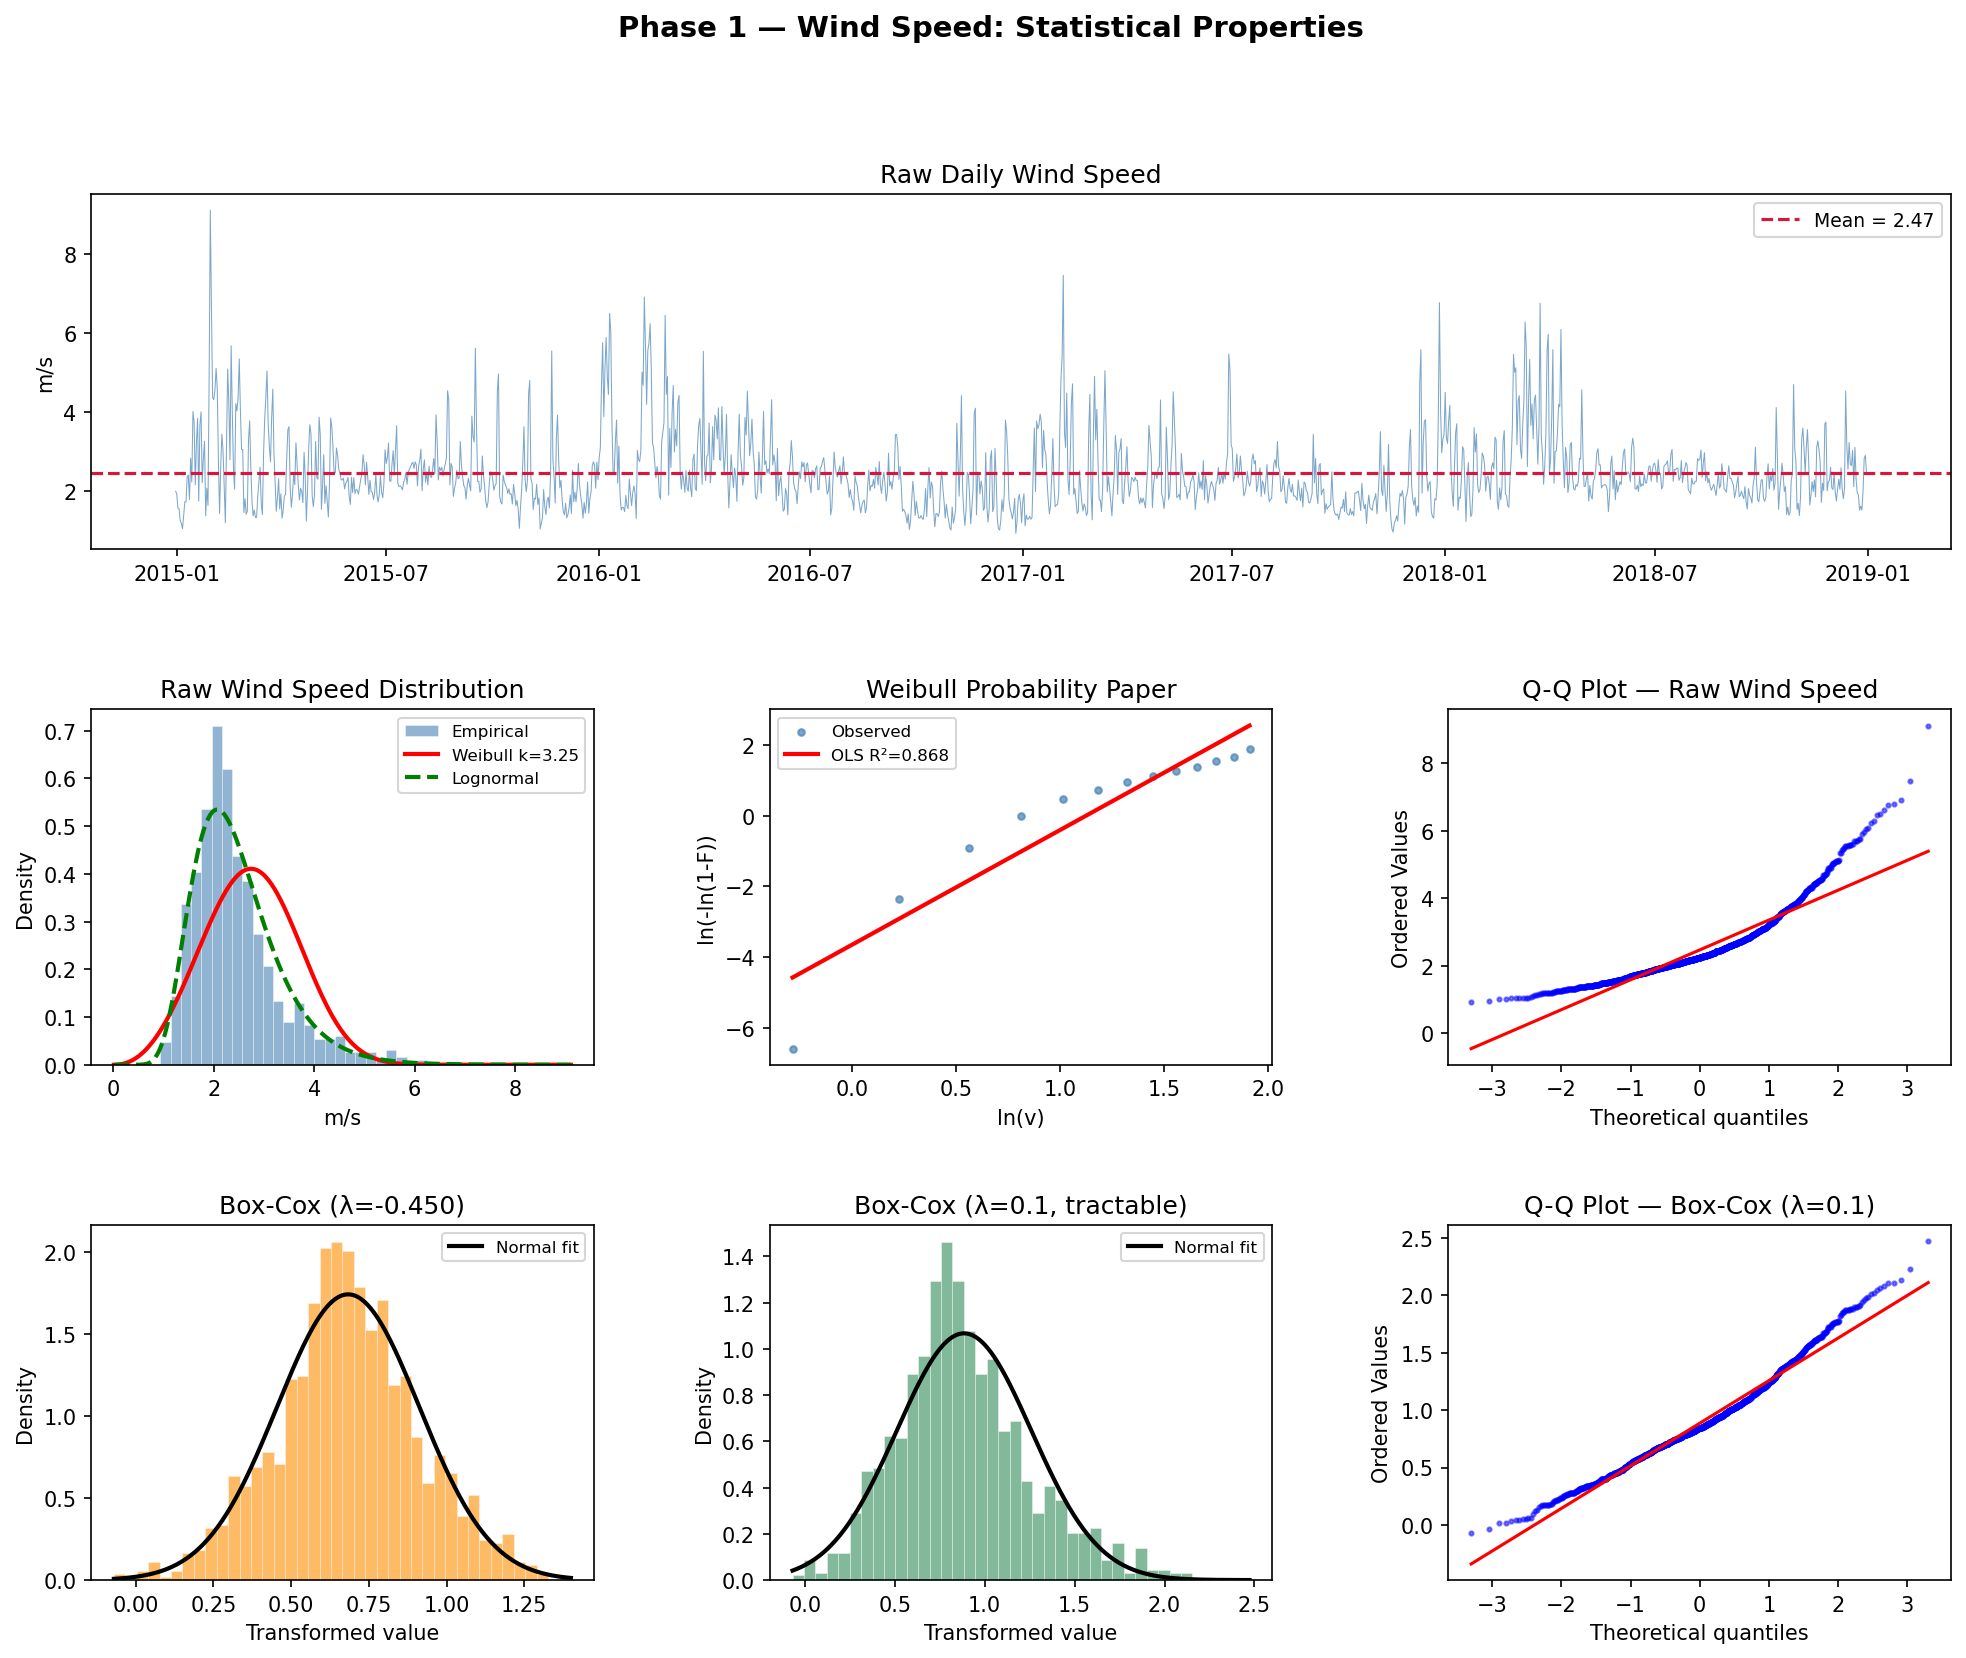
\includegraphics[width=\textwidth]{figures/phase1_wind_analysis.png}
\caption{Dataset A}
\end{subfigure}
\hfill
\begin{subfigure}{0.48\textwidth}
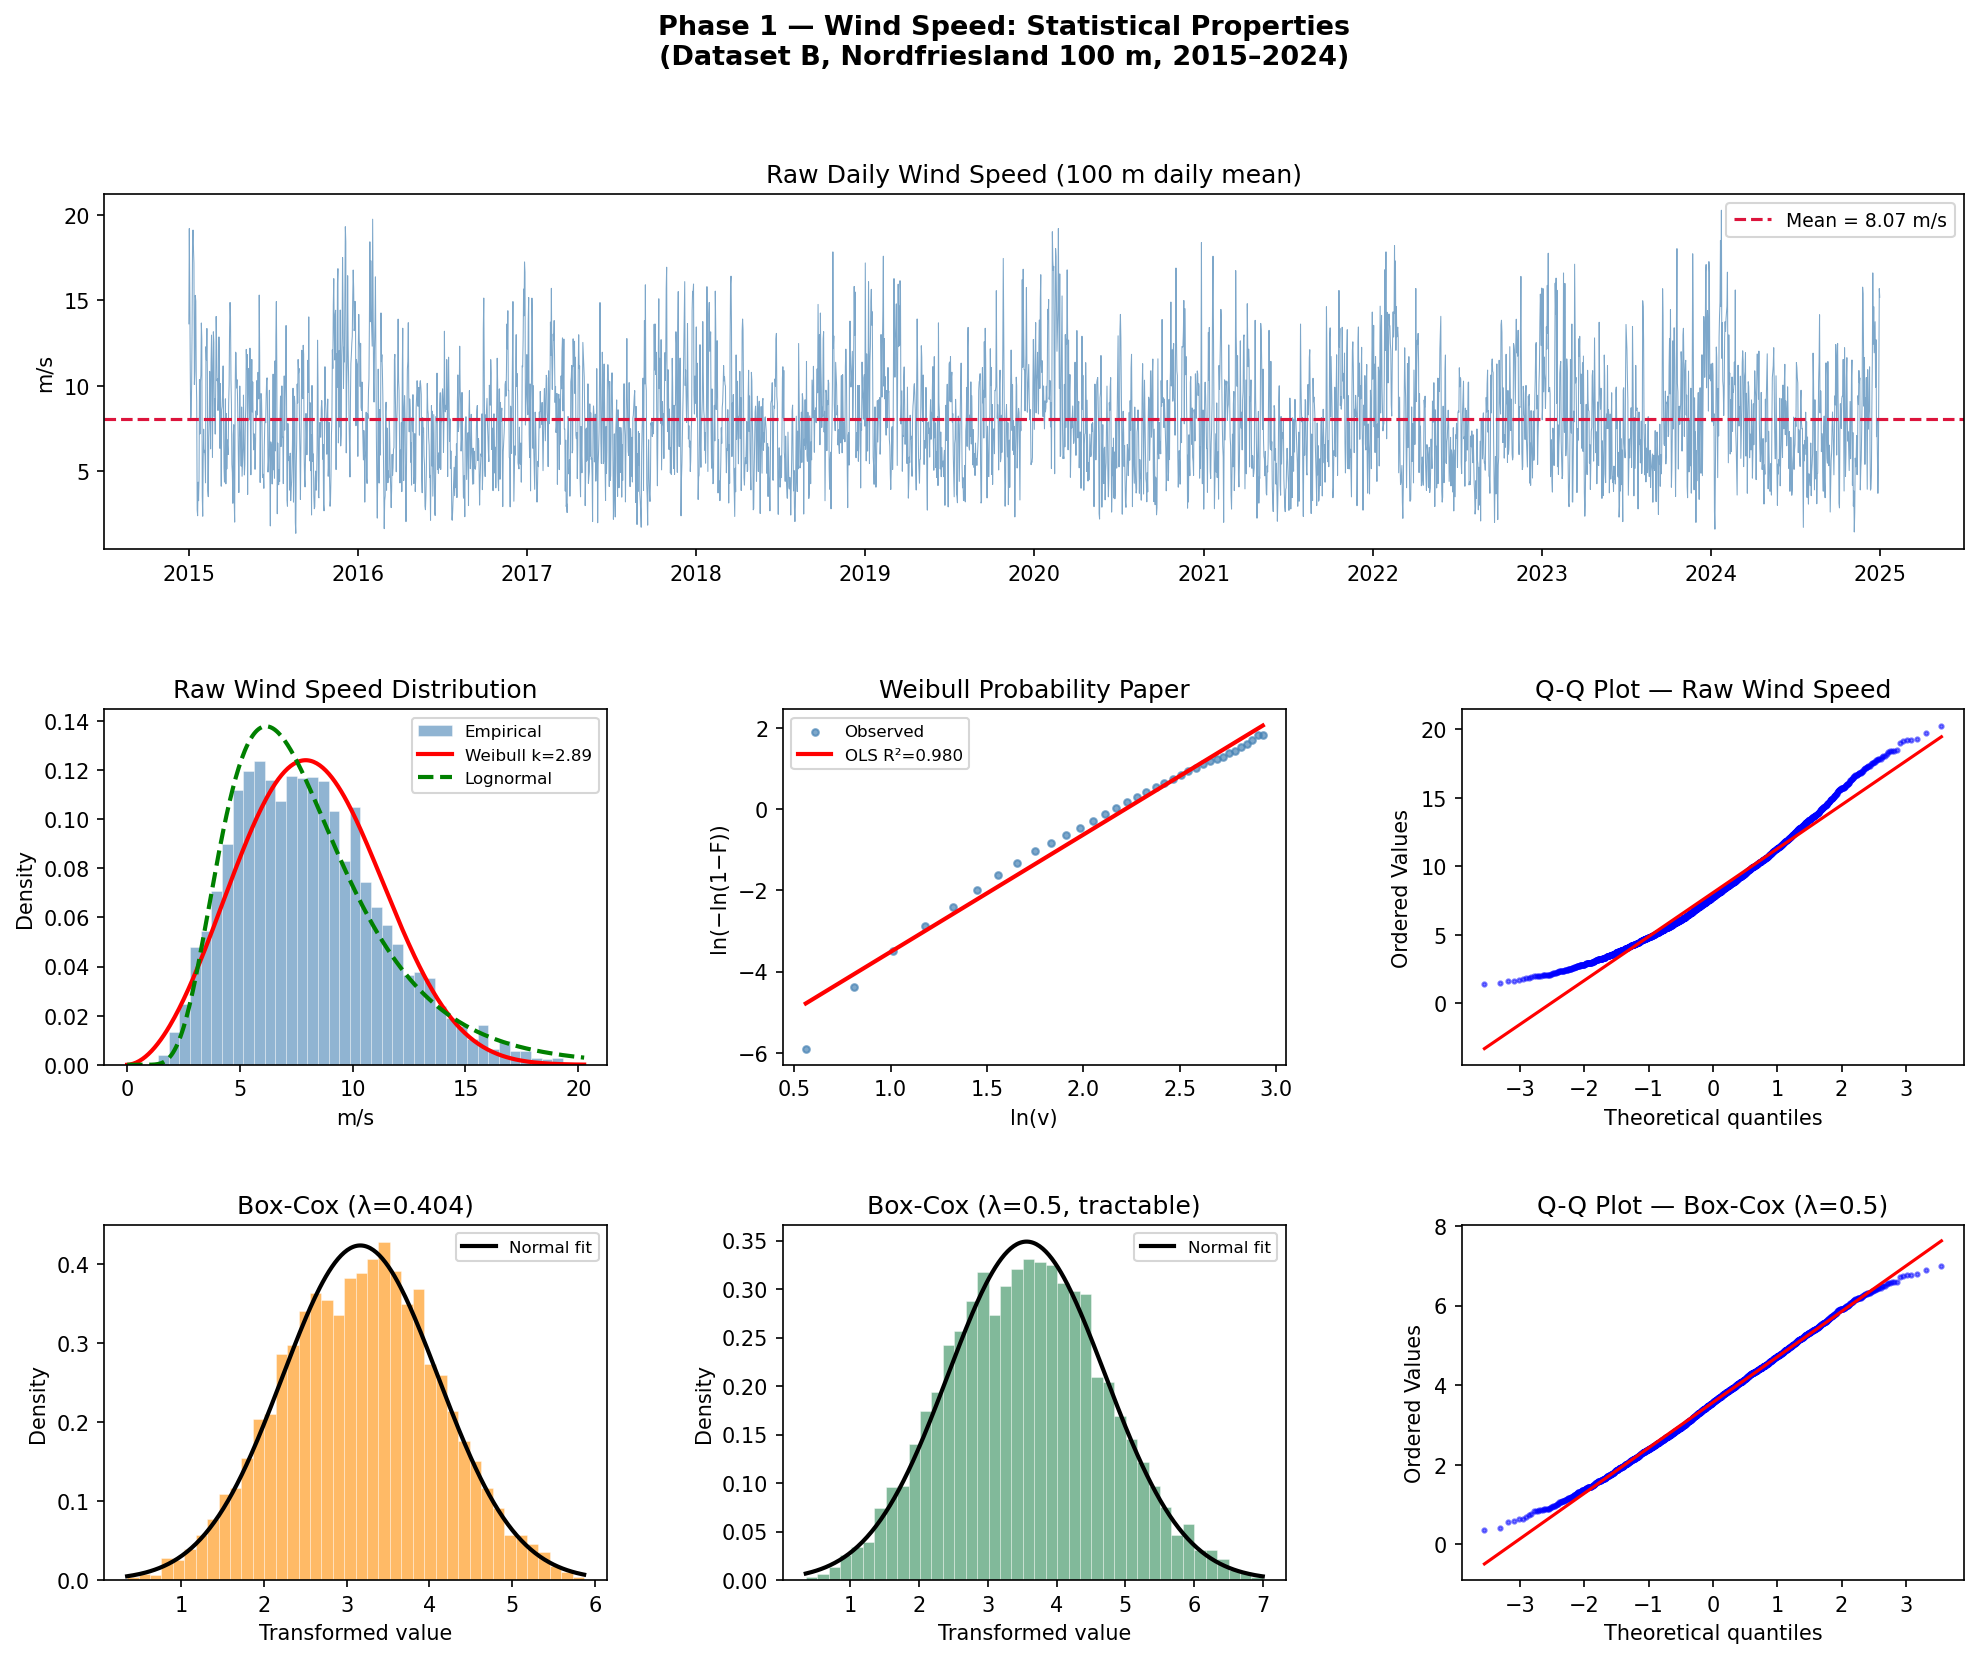
\includegraphics[width=\textwidth]{figures/phase1_B_wind_analysis.png}
\caption{Dataset B}
\end{subfigure}
\caption{Raw wind speed distribution and Box--Cox transformation, both datasets. Each panel is arranged in four rows, read top to bottom. \textbf{Row 1:} the raw daily wind speed time series, with the sample mean marked by a dashed line. \textbf{Row 2:} three diagnostics for the raw series -- a histogram with the fitted Weibull and lognormal densities overlaid, a Weibull probability-paper linearisation, and a quantile--quantile plot against the normal distribution, which shows the characteristic S-curve deviation of a right-skewed, heavy-tailed series. \textbf{Row 3:} histogram and quantile--quantile plot of the series after the likelihood-optimal Box--Cox transformation $\lambda_{\text{opt}}$. \textbf{Row 4:} histogram and quantile--quantile plot after the tractable Box--Cox value actually adopted ($\lambda = 0.1$ for Dataset A, $\lambda = 0.5$ for Dataset B), showing the residual departure from normality left by the tractability constraint discussed in Section~\ref{sec:phase1-boxcox}.}
\label{fig:phase1-wind}
\end{figure}

\subsection{Box--Cox Transformation}
\label{sec:phase1-boxcox}

The Box--Cox family $W^{(\lambda)}(t) = [W(t)^\lambda - 1]/\lambda$ (with $\ln W(t)$ for $\lambda = 0$) is fitted by maximising the profile log-likelihood under a normality assumption. For Dataset A, the likelihood-maximising value is $\lambda_{\text{opt}} = -0.450$, achieving near-perfect Gaussianisation (skewness $-0.005$, excess kurtosis $+0.128$, Jarque--Bera $p = 0.606$). For Dataset B, the optimum is $\lambda_{\text{opt}} = 0.404$, a much less extreme transformation, consistent with the higher hub-height mean wind speed producing a less severely skewed raw distribution. In both cases, the pricing formulas developed in Section~\ref{sec:phase4} and used throughout Chapter~3 require $1/\lambda$ to be a positive integer, so the likelihood optimum cannot be used directly. The requirement that $1/\lambda \in \mathbb{Z}^+$ is dictated by the analytical pricing formulas of Chapter~3. Pricing a forward contract requires computing the expected future wind speed in its original physical measure. Inverting the Box--Cox transformation requires taking the $(1/\lambda)$-th moment of a normal random variable, denoted $M_{1/\lambda}$ \citep{BenthSaltyteBenth2009}. If $1/\lambda$ were fractional, this expectation would lack a closed-form solution and risk generating complex numbers from negative intermediate states, destroying the model's analytical tractability. Following \citet{BenthSaltyteBenth2009}, who adopt $\lambda \in \{0.1, 0.2\}$ for the same CAR$(p)$ continuous-time embedding, $\lambda = 0.1$ is adopted for Dataset A and $\lambda = 0.5$ for Dataset B (Table~\ref{tab:boxcox}). The rounding cost is asymmetric: Dataset A's tractable value sits 0.35 units from its optimum and leaves a residual right skew (skewness $0.601$, Jarque--Bera $p \approx 0$), while Dataset B's tractable value sits only 0.10 units from its optimum and retains near-Gaussian shape (skewness $0.081$, KS $p = 0.091$).

\begin{table}[htbp]
\centering
\caption{Box--Cox transformation: optimal versus tractable $\lambda$.}
\label{tab:boxcox}
\begin{tabular}{l l l}
\toprule
& \textbf{Dataset A} & \textbf{Dataset B} \\
\midrule
$\lambda_{\text{opt}}$ (likelihood-maximising) & $-0.450$ & $0.404$ \\
Gaussianisation at $\lambda_{\text{opt}}$ (skew, JB $p$) & $-0.005$, $0.606$ & $-0.020$, $0.0002$ \\
$\lambda$ adopted (tractable, $1/\lambda \in \mathbb{Z}^+$) & $\mathbf{0.1}$ ($1/\lambda = 10$) & $\mathbf{0.5}$ ($1/\lambda = 2$) \\
Residual shape at adopted $\lambda$ (skew, JB $p$) & $0.601$, $\approx 0$ & $0.081$, $< 0.001$ \\
\bottomrule
\end{tabular}
\end{table}

\subsection{Seasonal Mean and Seasonal Variance}
\label{sec:phase1-seasonal}

Both the seasonal mean $\Lambda(t)$ and the seasonal variance $\sigma^2(t)$ are fitted as two-harmonic truncated Fourier series in calendar day-of-year, $\Lambda(t) = a_0 + \sum_{k=1}^2 [a_k \cos(2\pi k t/365) + b_k \sin(2\pi k t /365)]$ by ordinary least squares, and $\sigma^2(t) = c_0 + \sum_{k=1}^2 c_k \cos(2\pi k t/365)$ (cosine-only, reflecting the approximate symmetry of the variance cycle about its annual peak) fitted to the per-calendar-day empirical variance of the residuals $\varepsilon(t) = W^{(\lambda)}(t) - \Lambda(t)$. Table~\ref{tab:seasonal} reports both fits. The annual harmonic dominates the seasonal mean in both datasets ($b_1$ significant, $a_1$ not, for Dataset A; $a_1$ significant, $b_2$ not, for Dataset B), and the fitted $R^2$ is modest in both cases (0.126 and 0.103): most of the variance in daily wind speed is weather-driven, not calendar-driven, a finding consistent across both the four-year proxy sample and the ten-year reference sample. The seasonal-variance fit is more informative for the purposes of this thesis, since its intercept $C_0$ is the Fourier constant that enters the variance-swap pricing formula $K_{\text{var}}^B = h \times C_0$ of \citet{Tol1997}, used throughout Chapter~3: $C_0 = 0.13138$ for Dataset A versus $C_0 = 1.16277$ for Dataset B, an $8.85$-fold gap that Chapter~3's Value-of-Information analysis identifies as the dominant driver of the pricing error attributable to using the geographic proxy. Both datasets place peak seasonal variance in winter, though the relative modulation differs sharply: Dataset A's fitted $\sigma^2(t)$ ranges over $[0.032, 0.224]$, a winter-to-summer ratio of approximately $6.9$ to $1$, versus Dataset B's much milder range of $[0.944, 1.463]$, a ratio of approximately $1.55$ to $1$.

\begin{table}[htbp]
\centering
\small
\caption{Seasonal mean and seasonal variance Fourier fits, both datasets.}
\label{tab:seasonal}
\begin{tabular}{l l l}
\toprule
& \textbf{Dataset A} & \textbf{Dataset B} \\
\midrule
\multicolumn{3}{l}{\textit{Seasonal mean $\Lambda(t)$}} \\
$a_0$ & $0.88513$ (***) & $3.564$ (***) \\
$a_1$ (annual cos) & $-0.00544$ (n.s.) & $0.510$ (***) \\
$b_1$ (annual sin) & $0.16381$ (***) & $0.083$ (**) \\
$R^2$ & $0.126$ & $0.103$ \\
\midrule
\multicolumn{3}{l}{\textit{Seasonal variance $\sigma^2(t)$}} \\
$C_0$ (mean level) & $0.13138$ (***) & $1.16277$ (***) \\
$c_1$ (annual cos) & $0.09579$ (***) & $0.25933$ (***) \\
$c_2$ (semi-annual cos) & $-0.00332$ (n.s.) & $0.04077$ (n.s.) \\
$R^2$ & $0.226$ & $0.116$ \\
$\sigma^2(t)$ range & $[0.032, 0.224]$ & $[0.944, 1.463]$ \\
\bottomrule
\end{tabular}
\end{table}

\subsection{The Standardised Series $\widetilde W(t)$}
\label{sec:phase1-wtilde}

The standardised series $\widetilde W(t) = \varepsilon(t)/\sigma(t)$ is, by construction, close to zero-mean and unit-variance in both datasets (Dataset A: mean $0.001$, std.\ $0.967$; Dataset B: mean $-0.00003$, std.\ $1.005$), confirming that the centring and scaling steps were executed correctly. Neither series is yet white noise, however. The Ljung--Box statistic tests the joint null hypothesis that the first $m$ autocorrelations of a series are zero,
\begin{equation}
LBQ(m) = n(n+2)\sum_{k=1}^m \frac{\hat\rho(k)^2}{n-k} \ \sim\ \chi^2(m) \quad \text{under } H_0,
\end{equation}
where $\hat\rho(k)$ is the sample autocorrelation at lag $k$; applied to a series' squared values, the same statistic tests for conditional heteroskedasticity rather than serial correlation in levels. The test rejects the null of no serial correlation at every tested lag (5, 10, 20) for $\widetilde W(t)$ itself in both datasets ($p < 0.001$), and the same test applied to $\widetilde W(t)^2$ also rejects at every lag in both datasets ($p < 0.001$), indicating conditional heteroskedasticity beyond the deterministic seasonal variance already removed. These two findings are the direct motivation for the AR(4) mean model of Section~\ref{sec:phase2} and the GARCH(1,1) volatility model of Section~\ref{sec:phase3} respectively, and the pattern is identical across both datasets despite their very different sample lengths and measurement heights. This is evidence that the residual dynamics being modelled are a genuine feature of daily wind speed, not an artefact of one particular site or sample.

\begin{figure}[htbp]
\centering
\begin{subfigure}{0.48\textwidth}
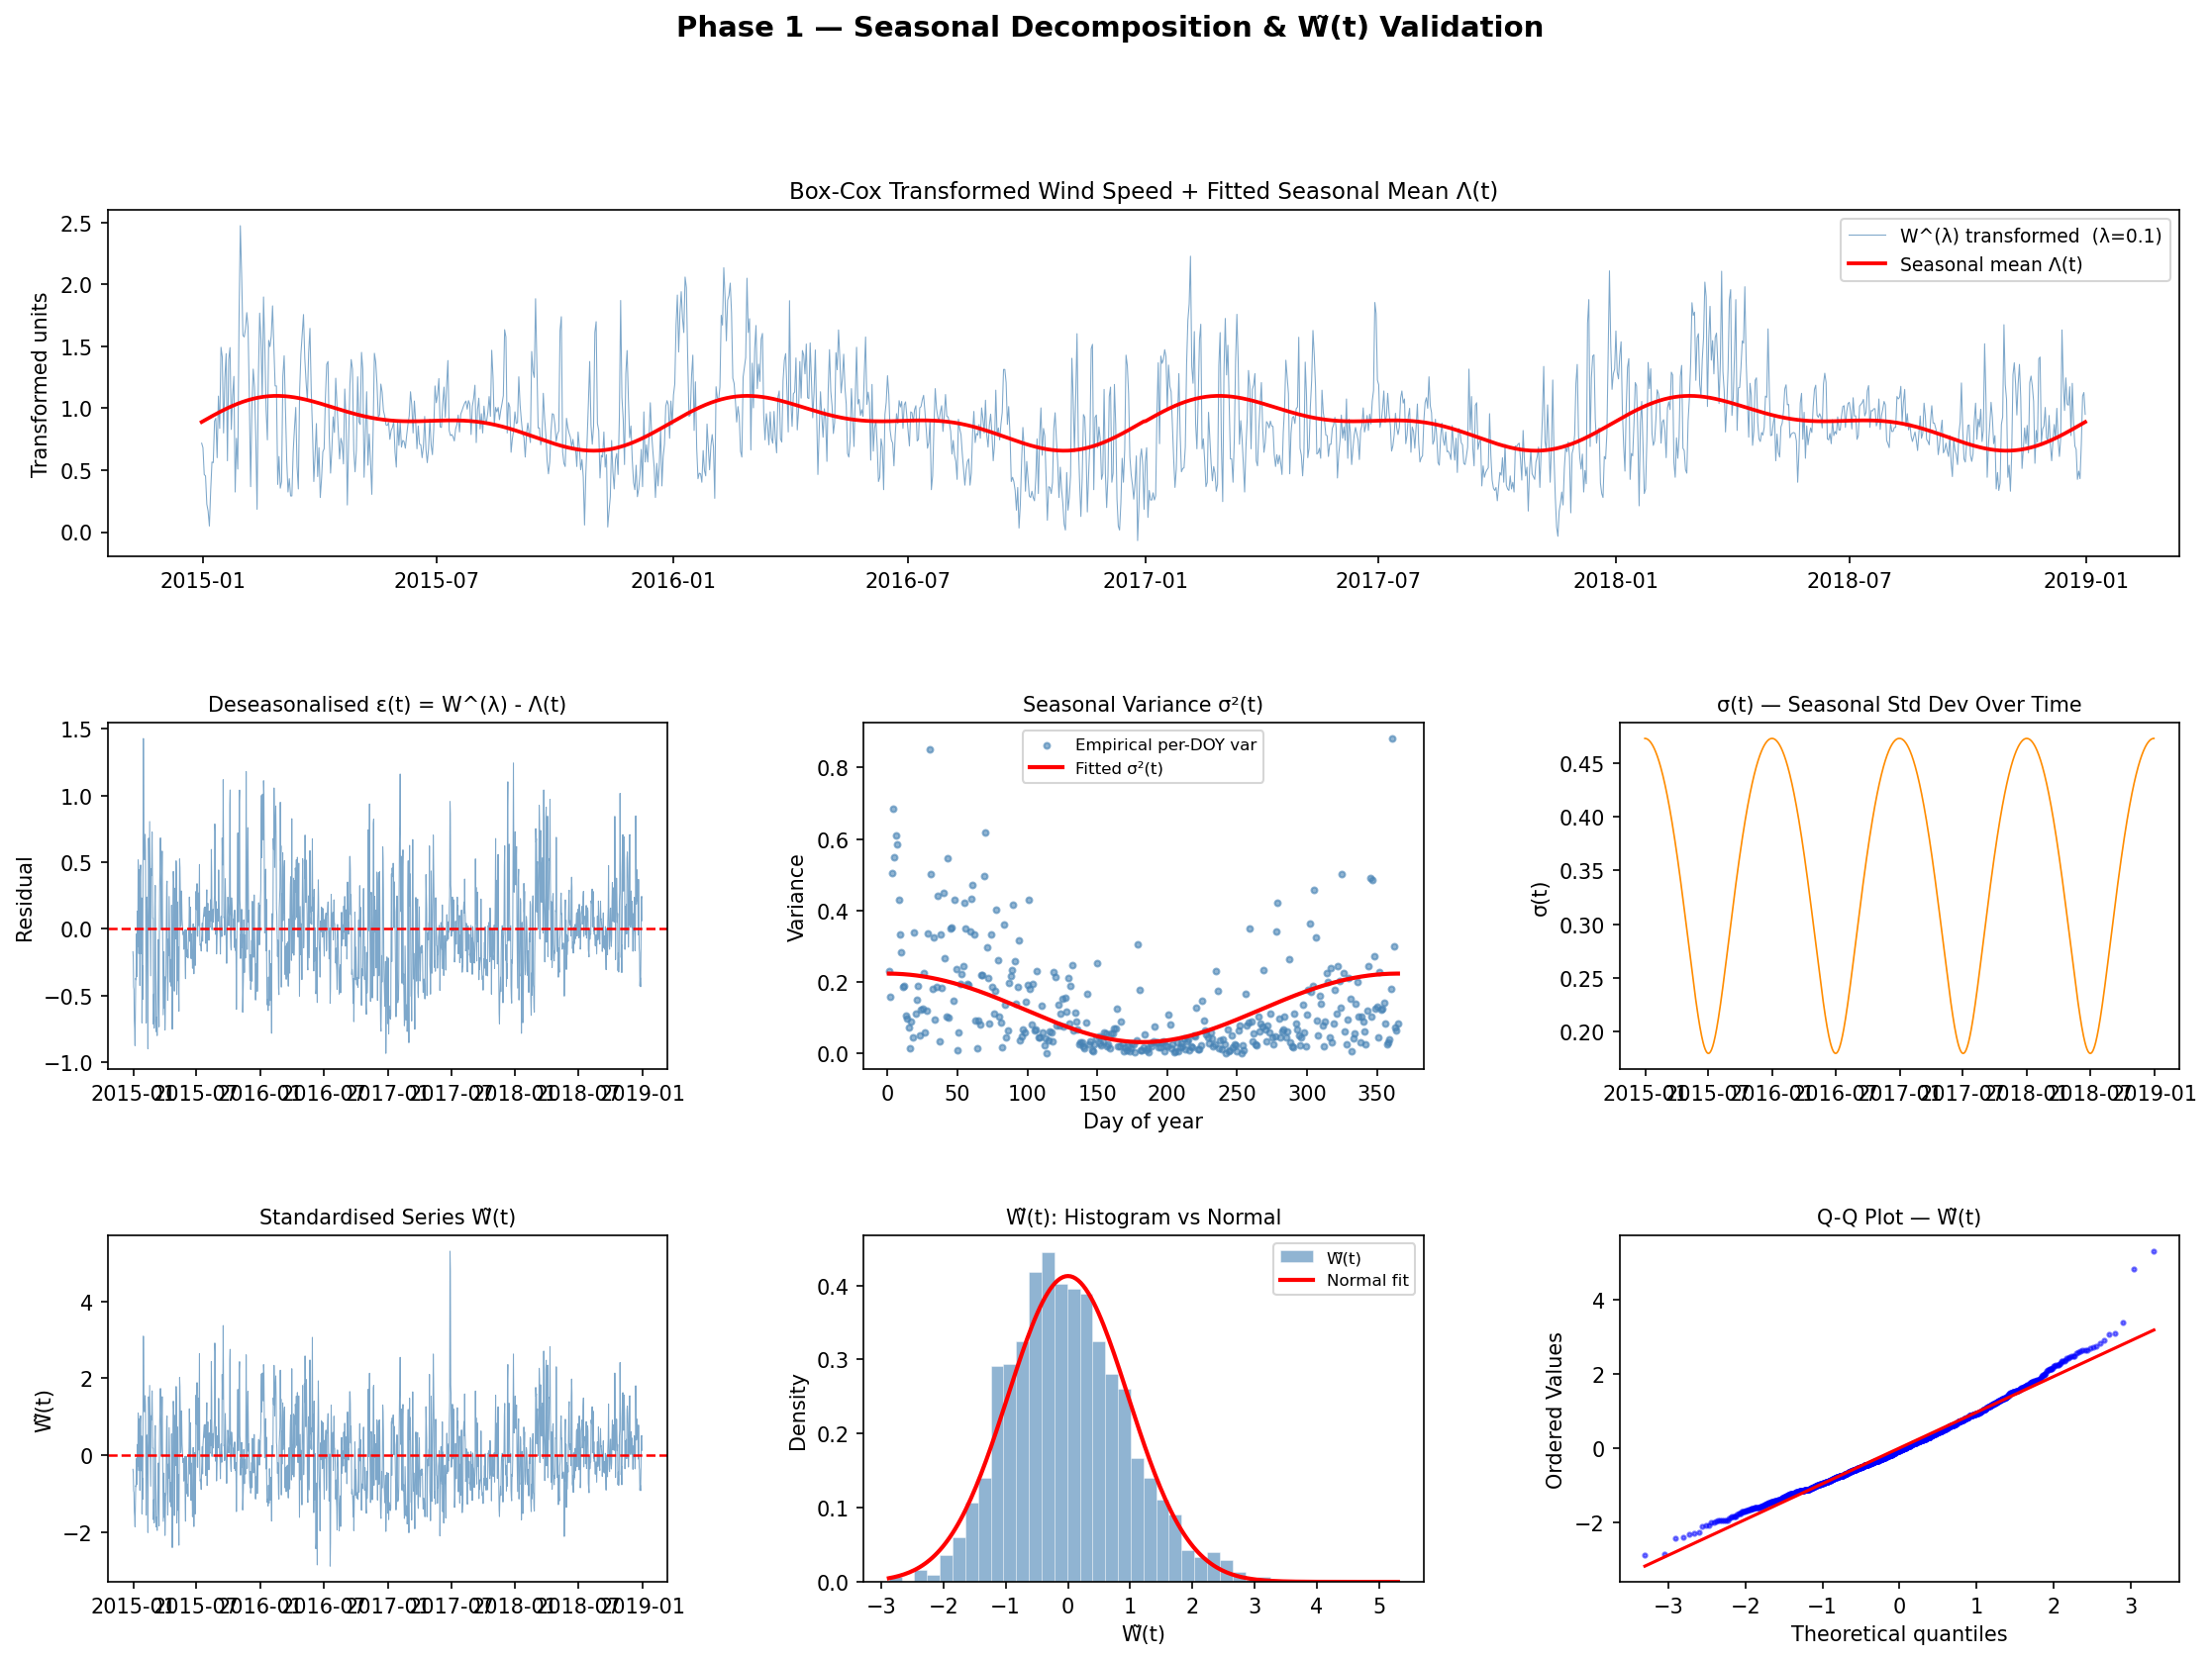
\includegraphics[width=\textwidth]{figures/phase1_seasonal_decomposition.png}
\caption{Dataset A}
\end{subfigure}
\hfill
\begin{subfigure}{0.48\textwidth}
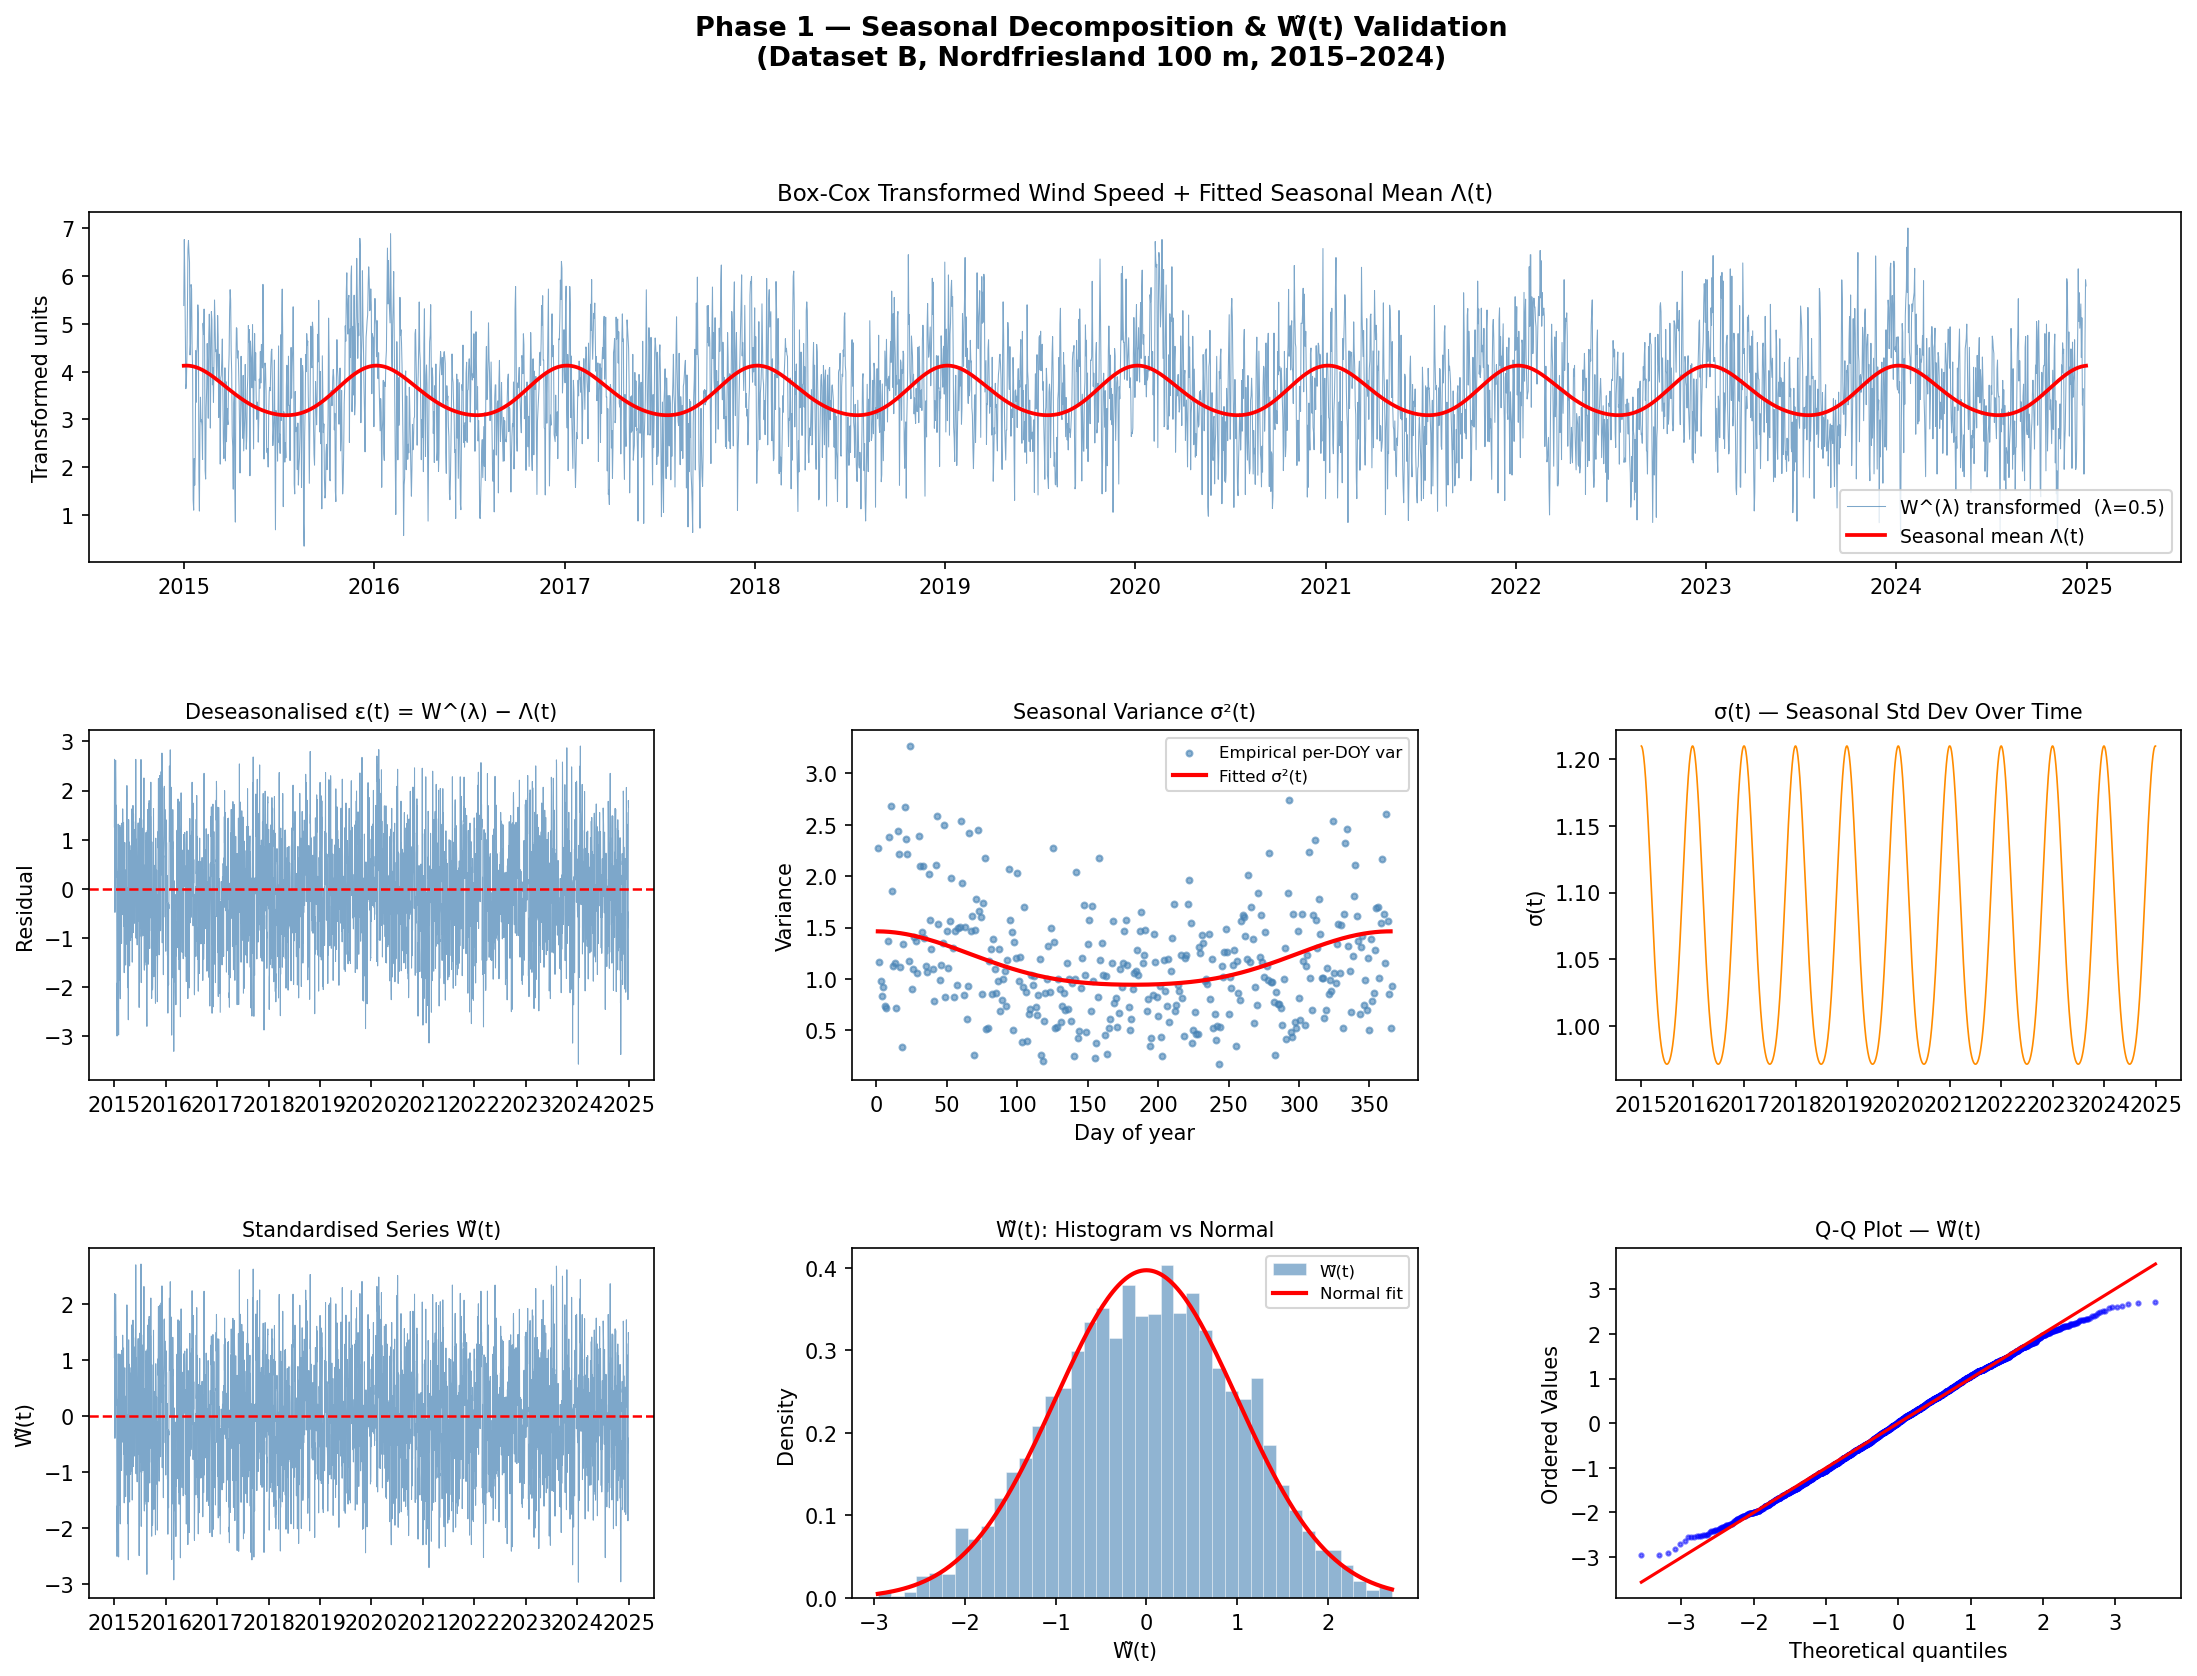
\includegraphics[width=\textwidth]{figures/phase1_B_seasonal_decomposition.png}
\caption{Dataset B}
\end{subfigure}
\caption{Seasonal decomposition and standardisation, both datasets. Each panel is arranged in three rows. \textbf{Row 1:} the transformed wind speed $W^{(\lambda)}(t)$ with the fitted seasonal mean $\Lambda(t)$ overlaid. \textbf{Row 2:} three panels -- the deseasonalised residuals $\varepsilon(t) = W^{(\lambda)}(t) - \Lambda(t)$; the empirical per-calendar-day variance (points) with the fitted Fourier seasonal-variance curve $\sigma^2(t)$ (line), showing the winter peak / summer trough pattern common to both datasets; and, third, an autocorrelation plot of the seasonal standard deviation curve across the calendar year, a supplementary panel not otherwise discussed in the main text. \textbf{Row 3:} the standardised series $\widetilde W(t)$, its histogram against a normal density, and a quantile--quantile plot, illustrating the residual serial dependence and non-normality quantified in Section~\ref{sec:phase1-wtilde}.}
\label{fig:phase1-seasonal}
\end{figure}

\section{Conditional Mean: AR(4)}
\label{sec:phase2}

The Ljung--Box evidence of Section~\ref{sec:phase1-wtilde} establishes that $\widetilde W(t)$ retains serial dependence. This section fits an autoregressive model to capture it.

\subsection{Order Selection}
\label{sec:phase2-order}

Both datasets exhibit a similar autocorrelation profile: a partial autocorrelation function (PACF) with clearly significant spikes at lags 1--3 and a markedly weaker, borderline value at lag 4 (Dataset A: PACF$_4 = 0.0311$, just inside the 95\% band; Dataset B: PACF$_4 = -0.0070$, effectively zero), with no significant structure beyond lag~4 in either series. An AIC/BIC grid search over AR($p$), $p = 1,\dots,6$, in fact selects AR(3) as the minimum-AIC model for \emph{both} datasets (Dataset A: AIC $= 3{,}432.24$ at $p=3$ versus $3{,}432.83$ at $p=4$, a difference of 0.59 units; Dataset B: AIC $=9{,}342.24$ at $p=3$ versus $9{,}344.04$ at $p=4$, a difference of 1.8 units), and in both cases the gap falls within the conventional two-point AIC band below which two models are considered statistically indistinguishable.

AR(4) is nonetheless retained as the operating specification in both datasets, on structural rather than statistical grounds: the continuous-time CAR(4) embedding of Section~\ref{sec:phase4} requires a companion matrix of dimension four, and the Euler-discretisation mapping from discrete AR coefficients $\{\beta_1,\dots,\beta_4\}$ to continuous CAR coefficients $\{\alpha_1,\dots,\alpha_4\}$, following \citet{BenthSaltyteBenth2009}, does not generalise to a three-lag or mixed ARMA specification. This is a deliberate trade-off, stated candidly here rather than left implicit: a fractionally-smaller-AIC three-lag model is set aside in favour of the four-lag model that the pricing framework of Chapter~3 actually requires, on the grounds that the statistical cost of doing so is, in both datasets, within the range normally treated as noise.

\subsection{AR(4) Coefficients}
\label{sec:phase2-coefs}

Table~\ref{tab:ar4} reports the fitted AR(4) coefficients for both datasets, estimated on the zero-mean series $\widetilde W(t)$ without an intercept. Both datasets show the coefficient magnitude declining with lag order and a positive, dominant $\beta_1$, but the two series differ in the sign of $\beta_4$ (Dataset A: $+0.0310$; Dataset B: $-0.0074$) and in the statistical significance of the higher lags: Dataset A's $\beta_2$ and $\beta_3$ are both significant at the 1\% level and $\beta_4$ is not significant ($p = 0.208$), while Dataset B's $\beta_3$ is only marginally significant ($p = 0.090$) and $\beta_4$ is clearly insignificant ($p = 0.660$). Neither discrepancy affects the modelling decision, since AR(4) is retained structurally regardless of the marginal significance of its highest lag, but both are reported here rather than smoothed over, since a coefficient that changes sign between the two datasets is a legitimate empirical finding, not a data-quality concern.

\begin{table}[htbp]
\centering
\caption{AR(4) coefficients, both datasets (OLS/MLE on $\widetilde W(t)$, no intercept).}
\label{tab:ar4}
\begin{tabular}{l r r r r}
\toprule
& \multicolumn{2}{c}{\textbf{Dataset A}} & \multicolumn{2}{c}{\textbf{Dataset B}} \\
\textbf{Coefficient} & \textbf{Estimate} & \textbf{$p$-value} & \textbf{Estimate} & \textbf{$p$-value} \\
\midrule
$\beta_1$ & $0.6299$ & $<0.001$ & $0.5324$ & $<0.001$ \\
$\beta_2$ & $-0.1443$ & $<0.001$ & $-0.0763$ & $<0.001$ \\
$\beta_3$ & $0.0926$ & $0.001$ & $0.0324$ & $0.090$ \\
$\beta_4$ & $0.0310$ & $0.208$ & $-0.0074$ & $0.660$ \\
\bottomrule
\end{tabular}
\end{table}

Both coefficient sets can be read against the New York daily wind-speed AR(4) fit reported by \citet{AlexandridisZapranis2013}: $\beta_1=0.362$, $\beta_2=-0.100$, $\beta_3=0.027$, $\beta_4=0.022$. Dataset A's coefficients are larger in magnitude than the New York benchmark at every lag. Dataset B's are larger at $\beta_1$ ($0.532$ versus $0.362$) and $\beta_3$ ($0.032$ versus $0.027$), but smaller at $\beta_2$ ($0.076$ versus $0.100$ in magnitude) and $\beta_4$ ($0.007$ versus $0.022$), so the comparison holds cleanly for the proxy dataset but only partially for the reference dataset. The dominant lag-1 coefficient, which carries most of the autoregressive structure in both series, is larger at both European sites than at the New York site, and this is attributed, in the underlying phase analysis, to a stronger lag-1 sample autocorrelation at both European sites (0.579 for Dataset A) than at the New York site ($\approx 0.36$), consistent with the sites' differing synoptic exposure rather than with any difference in modelling approach: the AR(4) specification itself is identical to the one used in the benchmark study.

For Dataset A, the characteristic roots of the fitted AR(4) polynomial have moduli $\{0.702, 0.470, 0.470, 0.200\}$, all inside the unit circle, confirming stationarity; the dominant root implies a mean-reversion half-life for the level of wind-speed anomalies of approximately 2.0 days. This is a materially faster reversion than the volatility half-life derived from the GARCH model in Section~\ref{sec:phase3} (41.6 and 38.3 days for Datasets A and B respectively): the \emph{level} of a wind-speed anomaly washes out within days, while the \emph{volatility regime} it occurred in persists for weeks, a distinction that recurs when the two dynamics are combined in Section~\ref{sec:phase4}.

\subsection{Residual Diagnostics}
\label{sec:phase2-diag}

Table~\ref{tab:ar4-diag} summarises the Ljung--Box tests on the AR(4) residuals $\hat\varepsilon(t)$ and on their squares. In both datasets, the serial-correlation test on levels passes comfortably at every lag ($p > 0.5$ throughout), confirming that AR(4) has removed the linear dependence identified in Section~\ref{sec:phase1-wtilde}. In both datasets, the test on squared residuals rejects the null of no remaining structure at conventional significance. This is corroborated by the Engle \citeyearpar{Engle1982} Lagrange-multiplier test for autoregressive conditional heteroskedasticity, which regresses squared residuals on their own lags, $\hat\varepsilon(t)^2 = \gamma_0 + \sum_{k=1}^q \gamma_k \hat\varepsilon(t-k)^2 + u(t)$, and tests the joint significance of $\gamma_1,\dots,\gamma_q$ via $\text{LM}(q) = nR^2 \sim \chi^2(q)$ under the null of no ARCH effects; the entry-residual ARCH-LM test is significant in both datasets (Dataset A: $\text{LM}(5) = 18.80$, $p = 0.0021$; Dataset B: $\text{LM}(5) = 16.58$, $p = 0.0054$). This is the expected and desired outcome at this stage: the AR(4) mean equation is adequate, and the conditional heteroskedasticity that remains is precisely what the GARCH(1,1) layer of Section~\ref{sec:phase3} is designed to capture.

\begin{table}[htbp]
\centering
\caption{AR(4) residual diagnostics, both datasets.}
\label{tab:ar4-diag}
\begin{tabular}{l r r}
\toprule
\textbf{Test} & \textbf{Dataset A} & \textbf{Dataset B} \\
\midrule
Ljung--Box $\hat\varepsilon(t)$, lag 20 ($p$) & $0.506$ & $0.511$ \\
Ljung--Box $\hat\varepsilon(t)^2$, lag 20 ($p$) & $0.0033$ & $0.2724^{\ast}$ \\
ARCH-LM(5) on entry residuals ($p$) & $0.0021$ & $0.0054$ \\
\bottomrule
\end{tabular}
\vspace{2pt}
{\footnotesize $^{\ast}$Dataset B's source analysis is internally inconsistent on its squared-residual diagnostics: the narrative text reports that the Ljung--Box test rejects homoskedasticity at lags 5 and 10 ($p = 0.0048$ and $0.0419$), while the lag-20 value tabulated there is $0.2724$ (a pass). The cell above reports the lag-20 value from the source table. Note that lags 5 and 10 rejections are the substantive finding motivating GARCH, regardless of the lag-20 outcome, and the ARCH-LM entry-residuals test (final row) is independently significant in both datasets.}
\end{table}

\subsection{Forecast Accuracy versus Persistence}
\label{sec:phase2-rmse}

Table~\ref{tab:ar4-rmse} reports one-step-ahead out-of-sample forecast accuracy against a persistence benchmark $\hat{\widetilde W}(t) = \widetilde W(t-1)$, using a walk-forward evaluation held out from the estimation sample. AR(4) reduces RMSE relative to persistence by 12.2\% in Dataset A and 13.8\% in Dataset B, and a Diebold--Mariano test \citep{DieboldMariano1995} rejects the null of equal predictive accuracy in both cases (Dataset A: $DM = -3.681$, $p = 0.0002$; Dataset B: $DM = -7.019$, $p < 0.001$). These are the frozen benchmark figures for the two datasets and are reused, without re-estimation, in the cross-dataset validation exercise of Chapter~3; a separate, later validation split reported there for Dataset B under the same Diebold--Mariano procedure (Section~3.2) uses a different train/test partition and yields a similar but not numerically identical improvement (13.6\%), a difference attributable entirely to the split rather than to any change in the fitted model, and reported explicitly as such where it recurs.

Two features of the Diebold--Mariano statistics themselves should be noted, since the figures quoted here differ from those reported for the same test in Chapter~3. The first is a sign convention. The evaluation used here defines the loss differential as $d_t = e^2_{\text{AR(4)}}(t) - e^2_{\text{persistence}}(t)$, so that a model outperforming the benchmark produces a \emph{negative} statistic; the Chapter~3 evaluation reverses the ordering, differencing the benchmark's squared error first, so the same outcome appears with a positive sign. The two are the same test reaching the same conclusion, and both reject the null at any conventional level. The second is magnitude: the statistics reported there are larger in absolute value ($8.26$ and $16.76$, against $3.681$ and $7.019$ here) because they are computed on the full standardised series rather than on the held-out partition used in this section. A Diebold--Mariano statistic scales with the square root of the evaluation sample, and the ratio of sample sizes alone accounts for most of what is observed in both datasets: $\sqrt{1462/220} \approx 2.6$ against an observed ratio of $2.2$ for Dataset A, and $\sqrt{3653/548} \approx 2.6$ against an observed $2.4$ for Dataset B.

One further property of the mean model is worth recording here, where the conditional mean is estimated, rather than leaving it to emerge in Chapter~3. The AR(4)+GARCH, CAR(4)+Gaussian and CAR(4)+NIG specifications developed in the following sections all inherit the AR(4) conditional mean unchanged: the GARCH layer of Section~\ref{sec:phase3} models the conditional variance of the residuals, and the CAR(4) embedding of Section~\ref{sec:phase4} is an exact continuous-time representation of the same mean dynamics, so none of the three alters the one-step-ahead point forecast. The four specifications are therefore observationally equivalent at a one-day horizon by construction, and differ only in their conditional-variance and tail representations. This is why the cross-dataset validation of Chapter~3 separates them on pricing and hedging criteria rather than on point-forecast accuracy, where no separation is available in principle.

\begin{table}[htbp]
\centering
\caption{AR(4) vs.\ persistence, one-step-ahead out-of-sample RMSE.}
\label{tab:ar4-rmse}
\begin{tabular}{l r r r r}
\toprule
& \multicolumn{2}{c}{\textbf{Dataset A}} & \multicolumn{2}{c}{\textbf{Dataset B}} \\
& \textbf{RMSE} & \textbf{MAE} & \textbf{RMSE} & \textbf{MAE} \\
\midrule
Persistence & $0.6856$ & $0.5214$ & $0.9955$ & $0.8054$ \\
AR(4) & $0.6017$ & $0.4706$ & $0.8580$ & $0.6950$ \\
Improvement & $12.2\%$ & --- & $13.8\%$ & --- \\
\bottomrule
\end{tabular}
\end{table}

\begin{figure}[htbp]
\centering
\begin{subfigure}{0.48\textwidth}
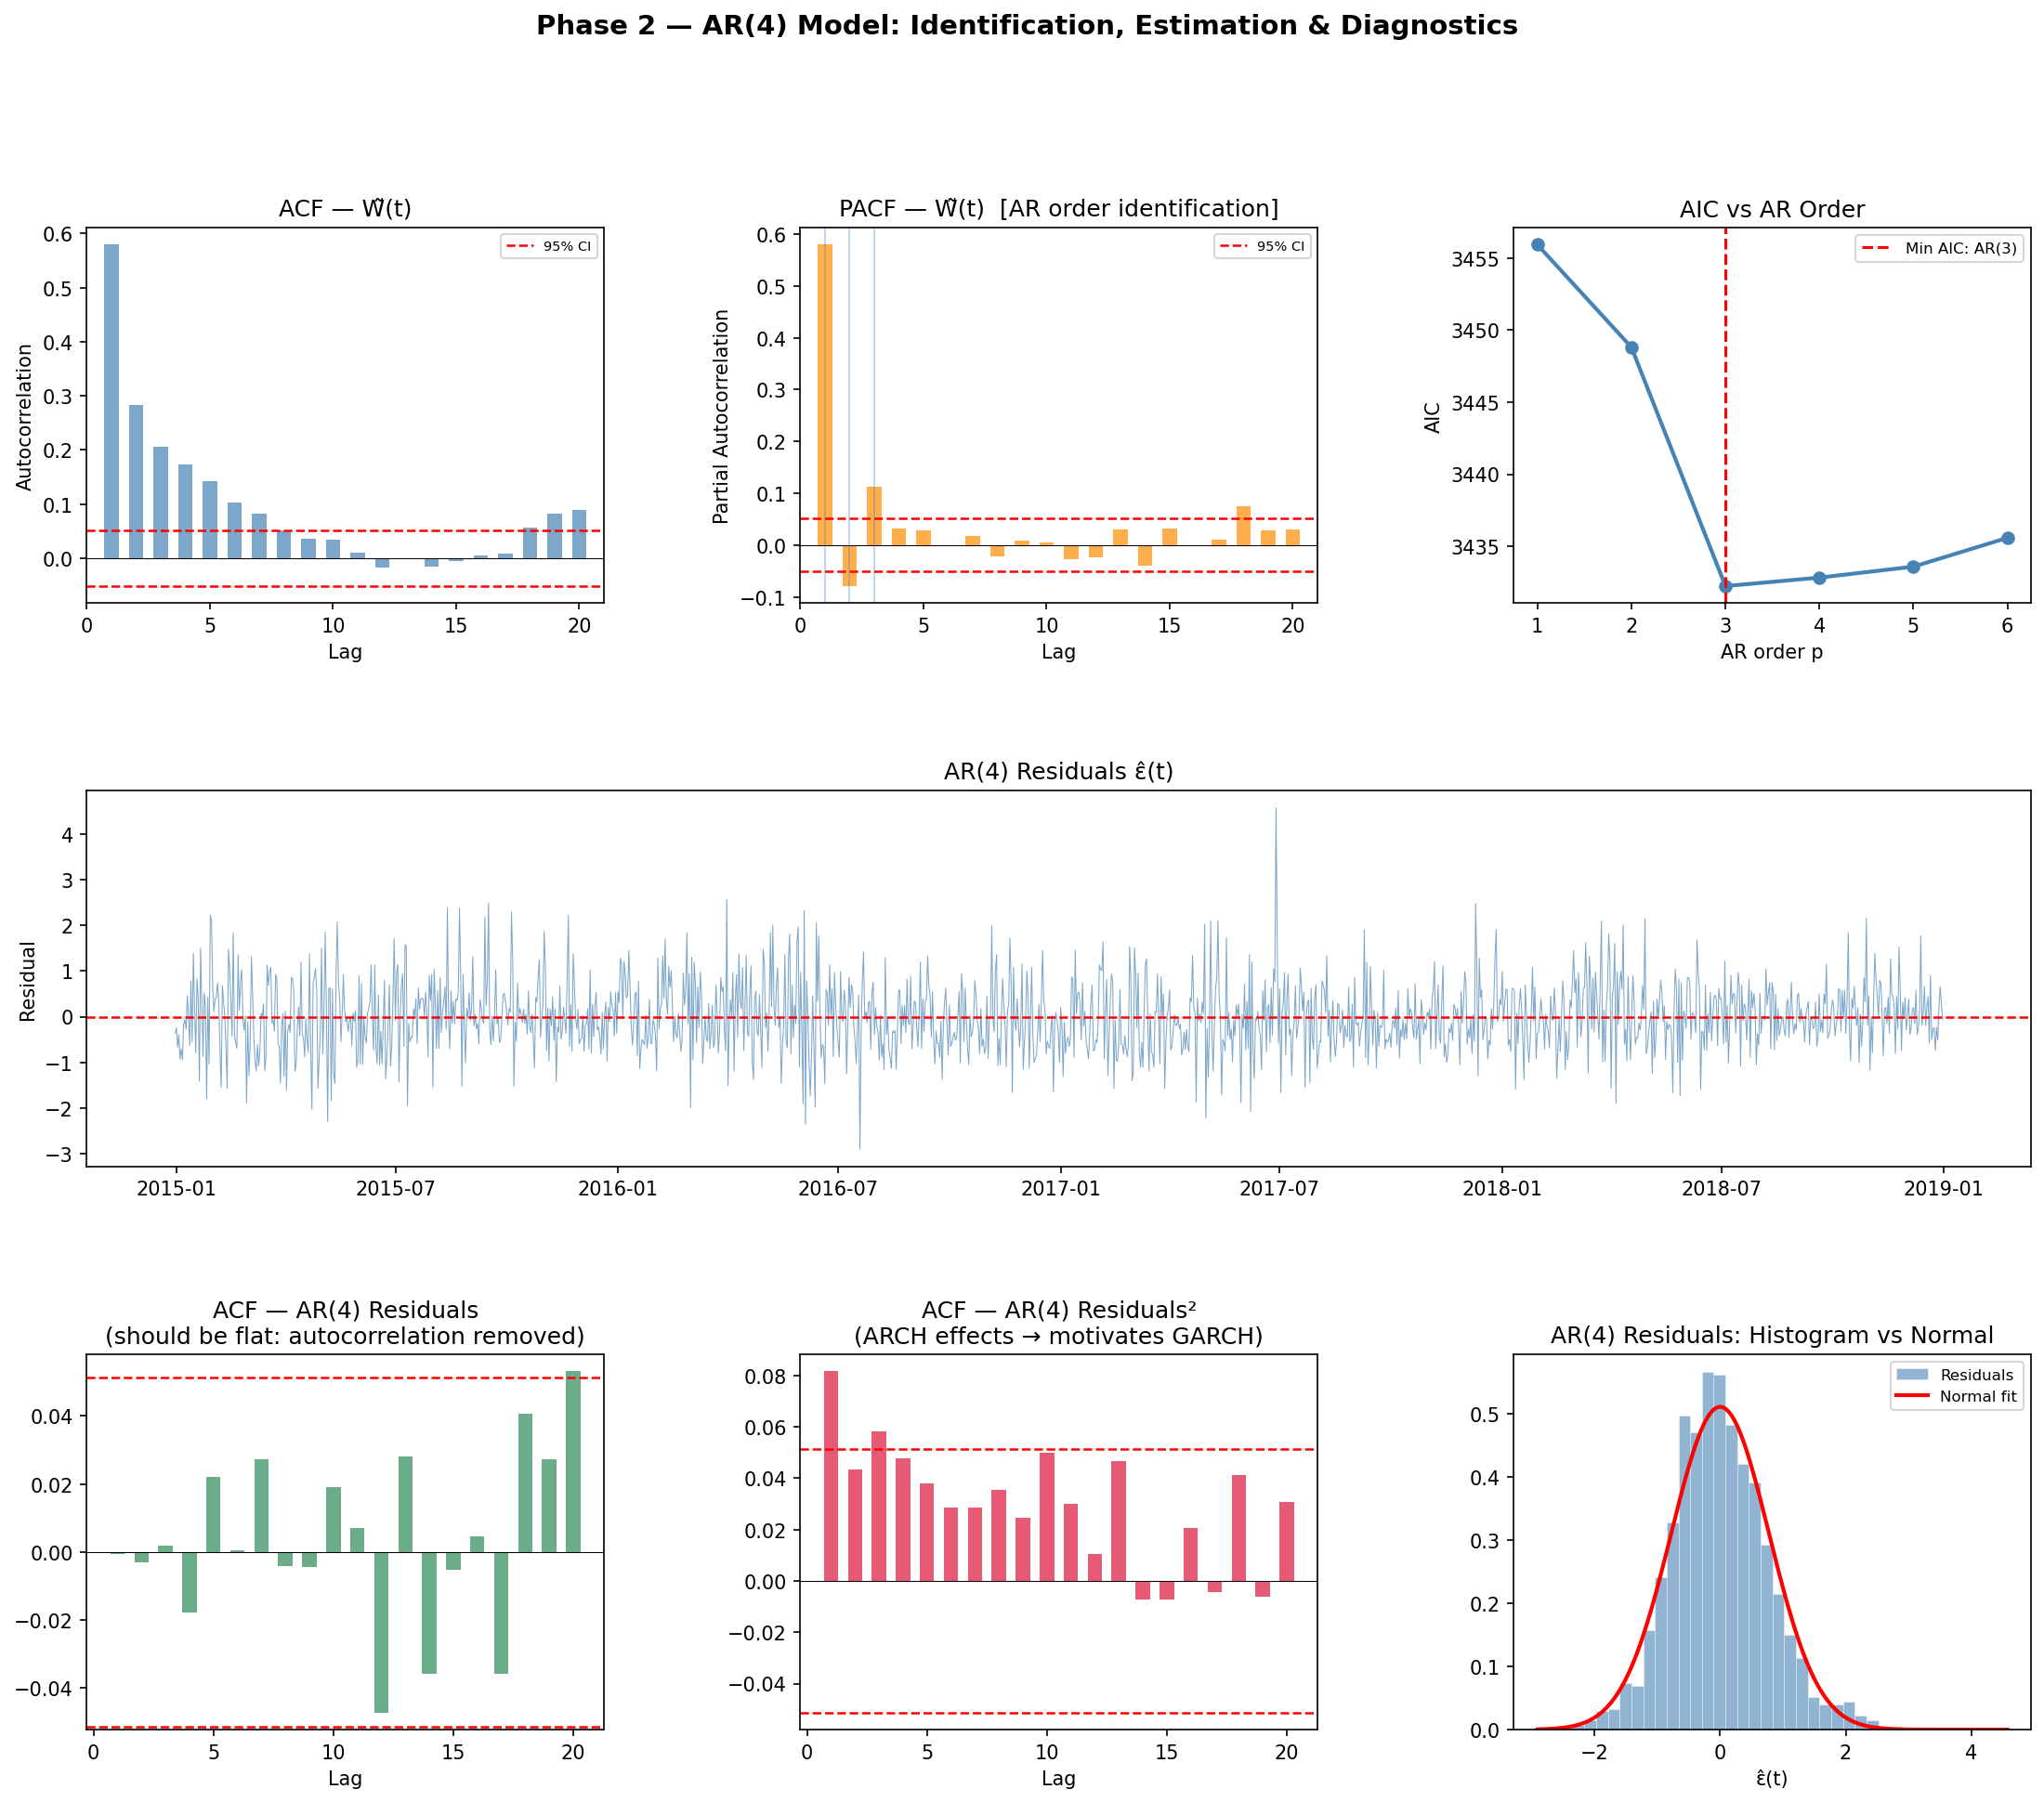
\includegraphics[width=\textwidth]{figures/phase2_ar4_diagnostics.png}
\caption{Dataset A}
\end{subfigure}
\hfill
\begin{subfigure}{0.48\textwidth}
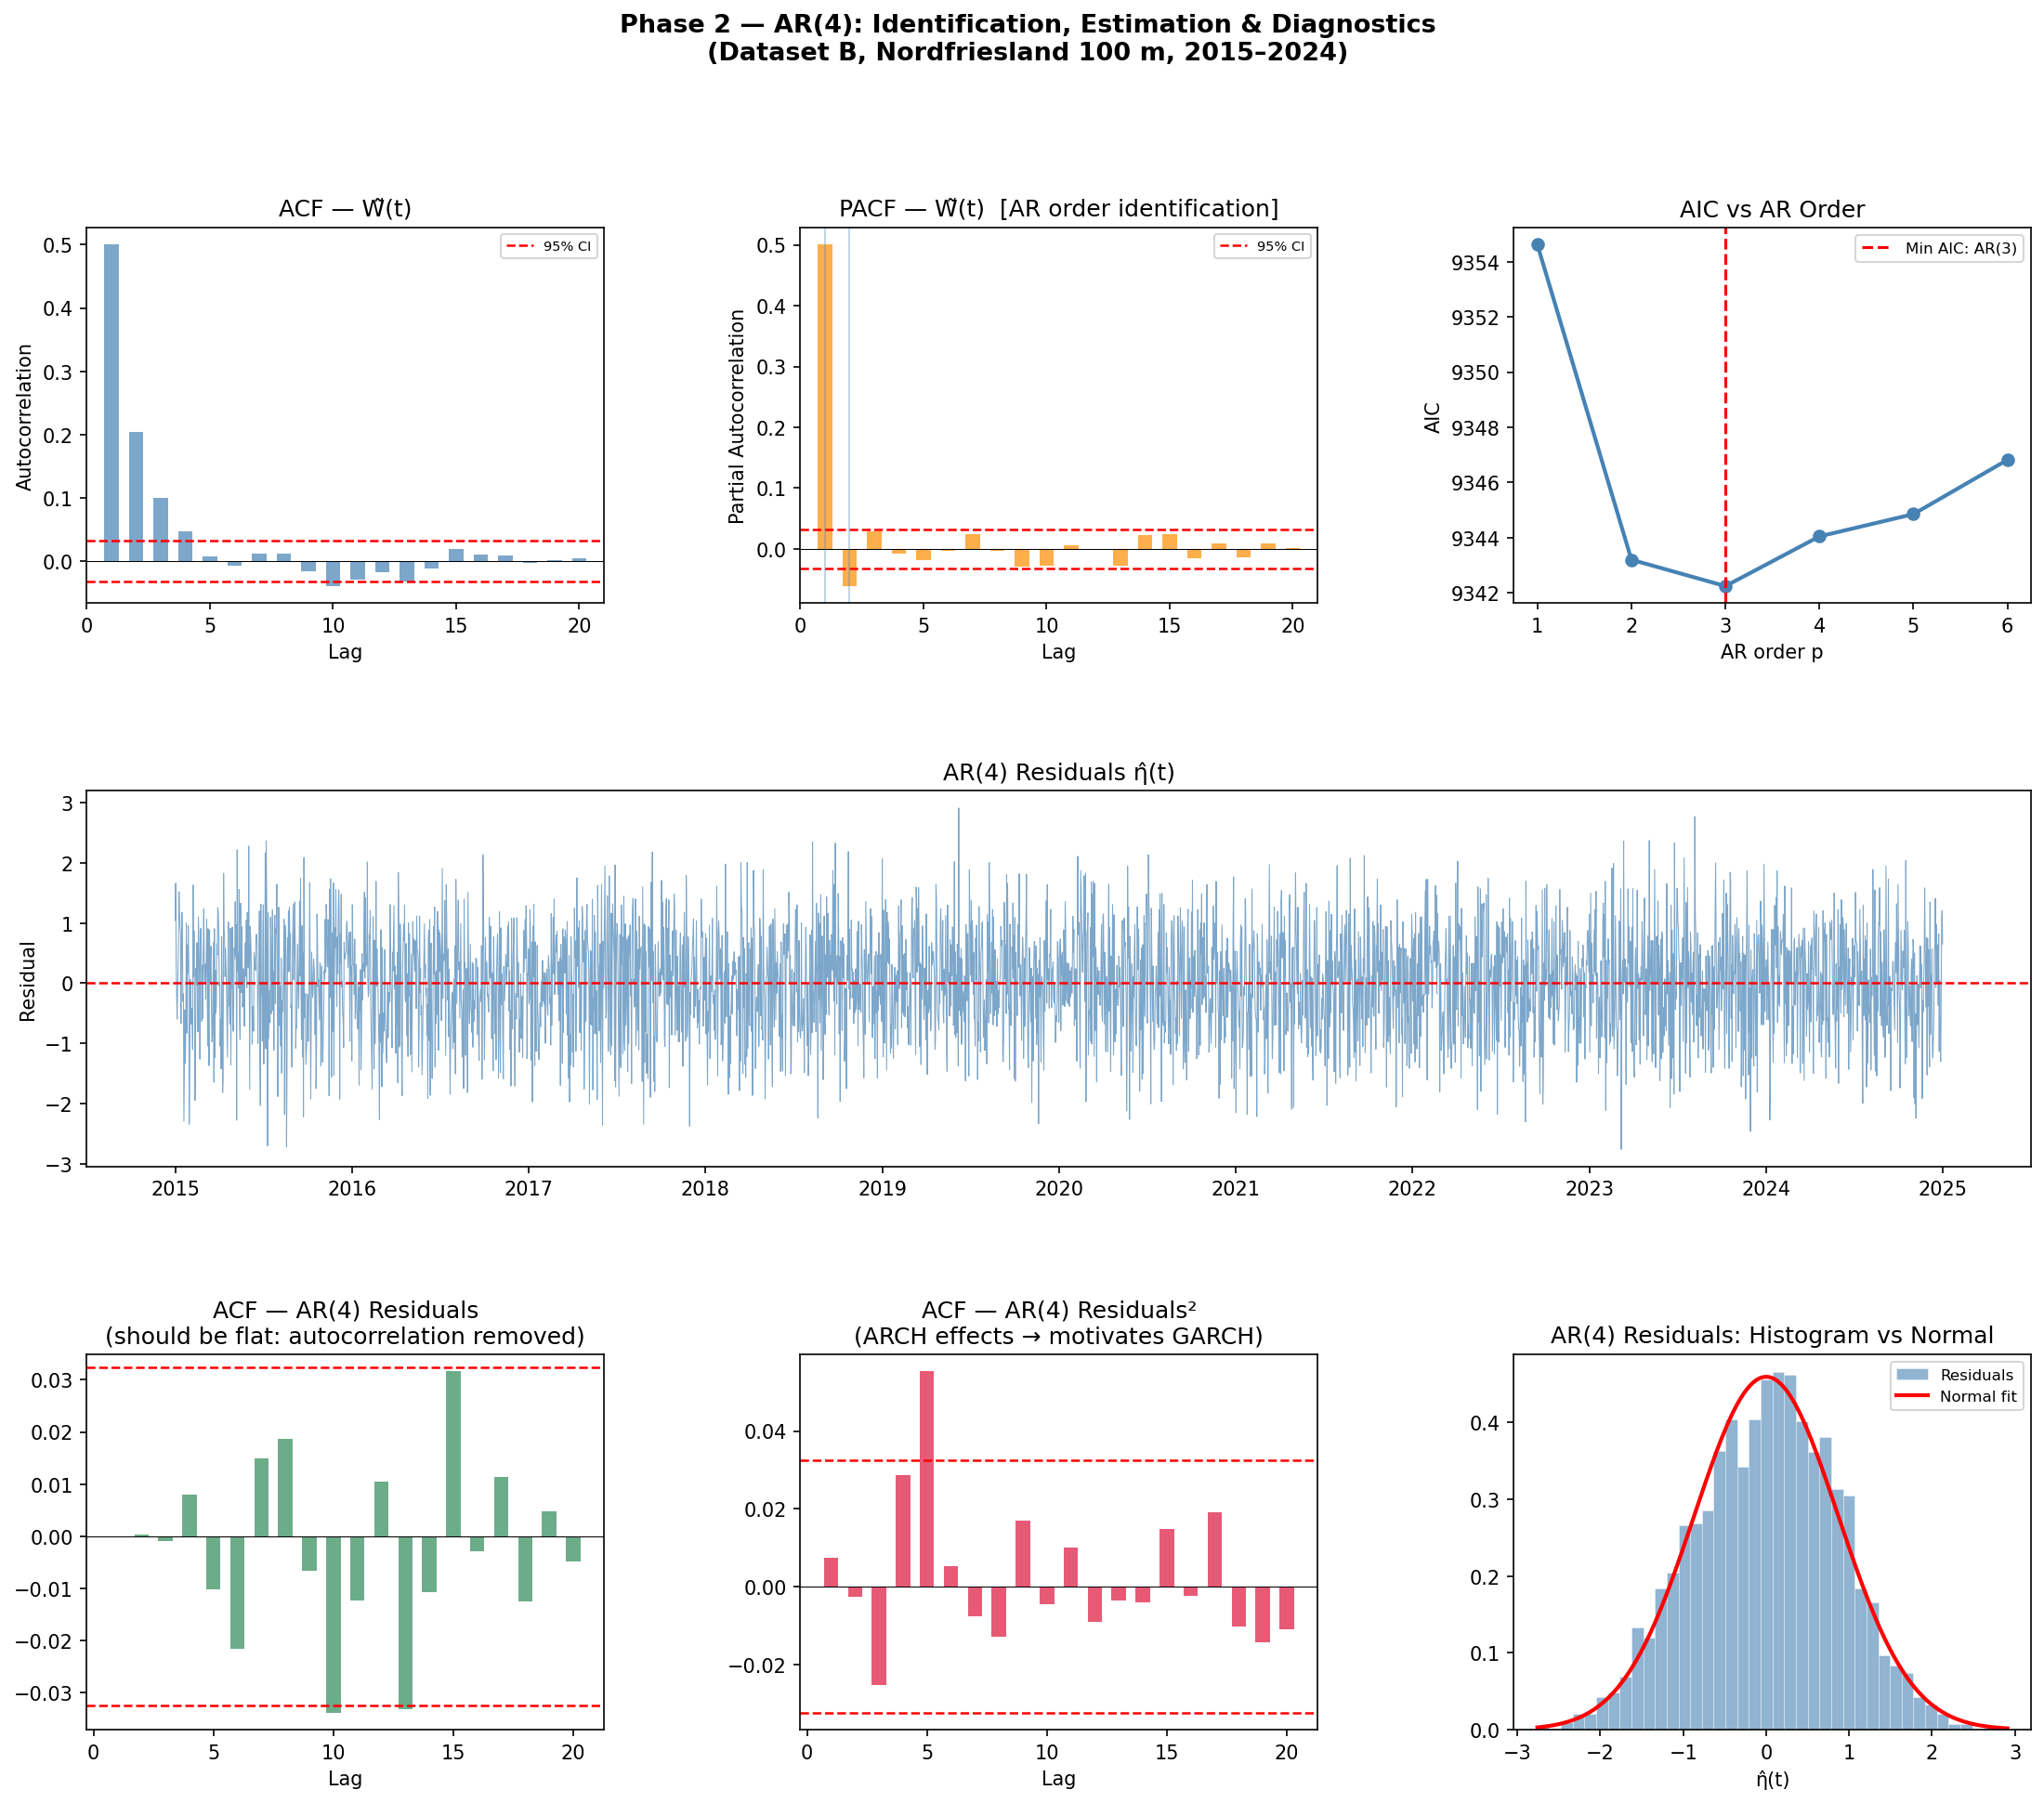
\includegraphics[width=\textwidth]{figures/phase2_B_ar4_diagnostics.png}
\caption{Dataset B}
\end{subfigure}
\caption{AR(4) identification and residual diagnostics, both datasets. Each panel is arranged in three rows. \textbf{Row 1:} three panels -- the autocorrelation function of $\widetilde W(t)$; its partial autocorrelation function, showing the decline to a borderline value at lag~4 discussed in Section~\ref{sec:phase2-order}; and the AIC grid search across candidate AR orders. \textbf{Row 2:} the time series of the AR(4) residuals $\hat\varepsilon(t)$. \textbf{Row 3:} three further panels, confirming that AR(4) has removed the linear serial dependence identified in Section~\ref{sec:phase1-wtilde} while conditional heteroskedasticity remains -- an autocorrelation-type diagnostic of $\hat\varepsilon(t)$; the corresponding diagnostic applied to $\hat\varepsilon(t)^2$, which stays visibly elevated and motivates the GARCH model of Section~\ref{sec:phase3}; and a histogram of $\hat\varepsilon(t)$ against a normal density.}
\label{fig:phase2-ar4}
\end{figure}

% Page break reproduces THESIS1_2.pdf pagination under any TeX distribution
% (TeX Live breaks here naturally; MiKTeX would otherwise fit this heading on p. 29).
\newpage
\subsection{Long Memory}
\label{sec:phase2-longmemory}

A natural question, given the literature reviewed in Section~1.3.2, is whether the residual dependence in $\widetilde W(t)$ decays exponentially, as a finite-order AR model assumes, or hyperbolically, as fractional integration would imply. The Geweke--Porter-Hudak (GPH) log-periodogram estimator regresses the log-periodogram of the series on the log of the frequency, $\ln I(\omega_j) = c - d\ln\left[4\sin^2(\omega_j/2)\right] + u_j$, over the $m = n^{0.6}$ lowest Fourier frequencies $\omega_j$, and tests $H_0: d = 0$ against fractional integration $d \neq 0$. It gives a fractional-differencing parameter of $\hat d = 0.119$ ($p = 0.208$) for Dataset A and $\hat d = -0.115$ ($p = 0.094$) for Dataset B. The interpretation of the two results is not symmetric, and the sign of the second matters. Long memory in the sense at issue here requires $0 < d < 0.5$; a negative $\hat d$ indicates anti-persistence, a hyperbolically decaying but sign-alternating dependence structure that is the opposite of long memory rather than a weak form of it. Dataset A therefore shows no long memory because it cannot reject $d = 0$ at all, and Dataset B shows none either, because although its $p$-value falls marginally inside a $p \le 0.10$ threshold, its point estimate carries the wrong sign for the hypothesis in question. Neither dataset provides evidence for fractional integration of the long-memory type at daily frequency.\footnote{The Dataset B source analysis reports an ARFIMA$(4,d,0)$ robustness fit alongside the GPH test, using $d = 0.010$ rather than the estimated $\hat d = -0.115$. The two are reconciled by the estimator's own admissibility constraint: the fitted value is passed through a clamp of the form $d = \max(0.01, \min(\hat d, 0.49))$ before the ARFIMA fit, so a negative estimate is floored at $0.01$ rather than used directly. The ARFIMA specification is consequently fitted at a value close to $d = 0$, and its reported AIC advantage over the AR(4) benchmark cannot be read as evidence of long memory, since the fractional-differencing parameter it uses was not the one the data produced. The same source document's Hurst-exponent figure caption states that its $R/S$ estimate ``confirms the absence of strong long-range dependence,'' consistent with the negative GPH estimate and with the conclusion reached in the main text, though in tension with a narrative sentence elsewhere in that document asserting that long memory ``is present.''} This reading is consistent with the wider literature: \citet{HaslettRaftery1989} and \citet{KavasseriSeetharaman2009} both find long memory to be primarily a feature of hourly or sub-daily wind data, so its absence after daily aggregation at both sites is the expected outcome rather than an anomaly. AR(4) is retained as the operating mean model for both datasets, now supported by the long-memory evidence rather than merely undisturbed by it, and for the structural reason given in Section~\ref{sec:phase2-order}.

\section{Conditional Volatility: GARCH(1,1)}
\label{sec:phase3}

Section~\ref{sec:phase2-diag} established that AR(4) residuals remain conditionally heteroskedastic in both datasets. This section models that heteroskedasticity directly, completing the two-component variance decomposition $\sigma^2_{\text{total}}(t) = \sigma^2_{\text{seasonal}}(t) \times h(t)$ that combines the deterministic Fourier seasonal variance of Section~\ref{sec:phase1-seasonal} with a GARCH$(1,1)$ conditional-variance multiplier $h(t)$, following \citet{Tol1997} and \citet{Bollerslev1986}.

\subsection{GARCH(1,1) Estimates}
\label{sec:phase3-estimates}

Table~\ref{tab:garch} reports the fitted GARCH(1,1) parameters for both datasets. In both cases $\beta$ dominates $\alpha$ by more than an order of magnitude (Dataset A: $\beta/\alpha \approx 31$; Dataset B: $\beta/\alpha \approx 165$), meaning that conditional variance is overwhelmingly carried forward from its own past level rather than driven by fresh shocks. \citet{Tol1997} characterises this pattern as typical of daily meteorological series, where volatility is governed by slow-moving synoptic weather regimes rather than the sharp, episodic jumps observed in financial return data. Dataset B's $\beta$ is both larger and more precisely estimated than Dataset A's, while its $\alpha$ is smaller and, unlike Dataset A's, not statistically significant on its own ($p = 0.210$); the constant $\omega$ is likewise insignificant for Dataset B ($p = 0.348$) but marginally significant for Dataset A ($p = 0.060$). Neither insignificant coefficient is dropped from either model, since the two-component variance decomposition requires all three GARCH parameters to reconstruct $h(t)$, and persistence, half-life, and the implied unconditional variance are computed from the fitted values regardless of the individual coefficients' marginal significance.

\begin{table}[htbp]
\centering
\caption{GARCH(1,1) estimates, both datasets.}
\label{tab:garch}
\begin{tabular}{l r r r r}
\toprule
& \multicolumn{2}{c}{\textbf{Dataset A}} & \multicolumn{2}{c}{\textbf{Dataset B}} \\
\textbf{Parameter} & \textbf{Estimate} & \textbf{$p$-value} & \textbf{Estimate} & \textbf{$p$-value} \\
\midrule
$\omega$ & $0.01004$ & $0.060$ & $0.01348$ & $0.348$ \\
$\alpha$ & $0.03105$ & $<0.001$ & $0.00590$ & $0.210$ \\
$\beta$ & $0.95242$ & $<0.001$ & $0.97618$ & $<0.001$ \\
\midrule
Persistence $\alpha + \beta$ & \multicolumn{2}{c}{$0.9835$} & \multicolumn{2}{c}{$0.9821$} \\
Half-life (days) & \multicolumn{2}{c}{$41.6$} & \multicolumn{2}{c}{$38.3$} \\
Implied unconditional variance & \multicolumn{2}{c}{$0.608$} & \multicolumn{2}{c}{$0.752$} \\
$h(t_0)$ (end of sample) & \multicolumn{2}{c}{$0.4137$} & \multicolumn{2}{c}{$0.7511$} \\
\bottomrule
\end{tabular}
\end{table}

Both models are covariance-stationary ($\alpha + \beta < 1$ in both cases). The volatility half-life (the time for a unit shock to conditional variance to decay to half its initial size, $\ln 2 / \ln[1/(\alpha+\beta)]$) is 41.6 days for Dataset A and 38.3 days for Dataset B, an order of magnitude longer than the mean-reversion half-life of the wind-speed \emph{level}, which is approximately two days for Dataset A on the discrete AR(4) roots of Section~\ref{sec:phase2-coefs} and $1.24$ days for Dataset B on the continuous-time eigenvalues of Section~\ref{sec:phase4-eigen}. Table~\ref{tab:garch-impulse} traces the resulting impulse-response decay $(\alpha+\beta)^{\text{lag}}$ explicitly: a unit shock to conditional variance still retains roughly 70\% of its initial effect after 20 days in both datasets (71.6\% for Dataset A, 69.7\% for Dataset B), and does not fall below one-quarter of its initial size until roughly three months out.

\begin{table}[htbp]
\centering
\caption{GARCH(1,1) impulse-response decay, $(\alpha+\beta)^{\text{lag}}$, both datasets.}
\label{tab:garch-impulse}
\begin{tabular}{l r r}
\toprule
\textbf{Lag (days)} & \textbf{Dataset A} & \textbf{Dataset B} \\
\midrule
0 & $100.0\%$ & $100.0\%$ \\
5 & $92.0\%$ & $91.4\%$ \\
10 & $84.6\%$ & $83.5\%$ \\
20 & $71.6\%$ & $69.7\%$ \\
30 & --- & $58.4\%$ \\
38 (Dataset B half-life) & --- & $50.0\%$ \\
42 (Dataset A half-life) & $50.0\%$ & --- \\
90 & $22.3\%$ & --- \\
\bottomrule
\end{tabular}
\end{table}

The distinction is physically meaningful and consistent across both datasets: an individual wind-speed anomaly washes out within days, but the volatility \emph{regime} it belongs to persists for weeks, consistent with the multi-week persistence of large-scale atmospheric circulation patterns such as blocking events and North Atlantic Oscillation phase.

\subsection{Two-Component Variance Decomposition}
\label{sec:phase3-decomp}

The key numeric outputs of this stage for the pricing work of Chapter~3 are two distinct products of the GARCH multiplier $h(t_0)$ with a seasonal-variance quantity, and the two must not be conflated. Chapter~3's synthetic variance swap prices under a piecewise-constant approximation, following \citet{Tol1997}, in which $h(t)$ is frozen at $h(t_0)$ for the life of the contract: $h(t_0) = 0.4137$ for Dataset A and $h(t_0) = 0.7511$ for Dataset B.

The first quantity is the \emph{pointwise} total variance at the pricing date, $\sigma^2_{\text{total}}(t_0) = h(t_0) \times \sigma^2_{\text{seasonal}}(t_0)$, which governs the conditional-variance term structure of Section~\ref{sec:phase4-forecast}. For Dataset A this is $0.4137 \times 0.2239 = 0.0926$, using the pointwise seasonal variance at $t_0$ recorded in Section~\ref{sec:phase4-c0}, and reproduces the frozen anchor exactly. The second is the \emph{annualised} fair strike $K_{\text{var}}^B = h(t_0) \times C_0$, which replaces the pointwise seasonal variance with its annual Fourier mean $C_0$, because the first and second harmonics of $\sigma^2_{\text{seasonal}}(t)$ integrate to zero over a full contract year. For Dataset A this is $0.4137 \times 0.13138 = 0.0544$, the figure carried into Chapter~3. The distinction matters because the two differ by a factor of roughly $1.7$ for Dataset A, and because it is the annual mean $C_0$, not the pricing-date value, that the closed-form strike requires.

The seasonal pattern of $h(t)$ itself differs qualitatively between the two datasets. In Dataset A, $h(t)$ is markedly higher in late spring and early summer (monthly mean up to $0.768$ in June) than in autumn (as low as $0.465$ in October), a pattern that runs in the opposite direction to the seasonal variance $\sigma^2_{\text{seasonal}}(t)$, which peaks in winter; the two effects partially offset each other in the total variance $\sigma^2_{\text{total}}(t)$, so that pricing from the seasonal component alone, ignoring $h(t)$, would overstate summer volatility and understate the GARCH contribution in the shoulder months. In Dataset B, by contrast, $h(t)$ shows only a mild seasonal range (monthly means between $0.734$ and $0.770$), and most of its time variation is carried by shock persistence rather than calendar effects; total variance in Dataset B therefore tracks the seasonal component more directly than in Dataset A.

\subsection{Standardised Residual Diagnostics}
\label{sec:phase3-diag}

Table~\ref{tab:garch-diag} reports diagnostics on the standardised residuals $z(t) = \hat\varepsilon(t)/\sqrt{h(t)}$. Both datasets pass the Ljung--Box test for remaining serial correlation and remaining ARCH effects on $z(t)$ and $z(t)^2$ at conventional significance, confirming that GARCH(1,1) is an adequate specification for the conditional-variance dynamics in both cases. The two datasets diverge, however, in the shape of their standardised residuals: Dataset A's $z(t)$ is leptokurtic (excess kurtosis $+1.12$), with a heavy right tail driven substantially by a single extreme observation (28~June~2017, $z = +5.79$), while Dataset B's is mildly platykurtic (excess kurtosis $-0.28$), thinner-tailed than Gaussian. Neither departure is treated as invalidating the GARCH(1,1) specification, since both series pass the joint white-noise tests that matter for the volatility model itself, but the residual non-normality, in whichever direction, motivates the heavy-tailed Normal-Inverse-Gaussian treatment introduced in Section~\ref{sec:phase4-nig}. One further asymmetry is worth flagging directly rather than smoothing over: an ARCH-LM test on Dataset B's standardised residuals is marginally significant at 5\% ($p = 0.0185$), where the equivalent test on Dataset A's standardised residuals passes comfortably ($p = 0.821$); Dataset B's own summary narrative characterises its residuals as passing validation cleanly, a characterisation that this specific test result only partially supports. This is not an artefact of a different evaluation window: the Phase~7 validation that Chapter~3 draws on recomputes the same test on the same standardised residuals and returns the identical statistic and $p$-value ($\mathrm{LM}(5) = 13.58$, $p = 0.0185$). It should be noted that the Phase~7 write-up nevertheless describes this test as returning $p > 0.05$ and records the residuals as passing all diagnostics, a characterisation that its own executed output does not support; the value reported here and carried into Chapter~3 is the computed one.

\begin{table}[htbp]
\centering
\caption{GARCH(1,1) standardised-residual diagnostics, both datasets.}
\label{tab:garch-diag}
\begin{tabular}{l r r}
\toprule
\textbf{Test} & \textbf{Dataset A} & \textbf{Dataset B} \\
\midrule
Excess kurtosis of $z(t)$ & $+1.12$ (leptokurtic) & $-0.28$ (platykurtic) \\
Ljung--Box $z(t)$, lag 20 ($p$) & $0.765$ & $0.503$ \\
Ljung--Box $z(t)^2$, lag 20 ($p$) & $0.988$ & $0.283$ \\
ARCH-LM(5) on $z(t)$ ($p$) & $0.821$ & $0.0185$ \\
\bottomrule
\end{tabular}
\end{table}

\begin{figure}[htbp]
\centering
\begin{subfigure}{0.48\textwidth}
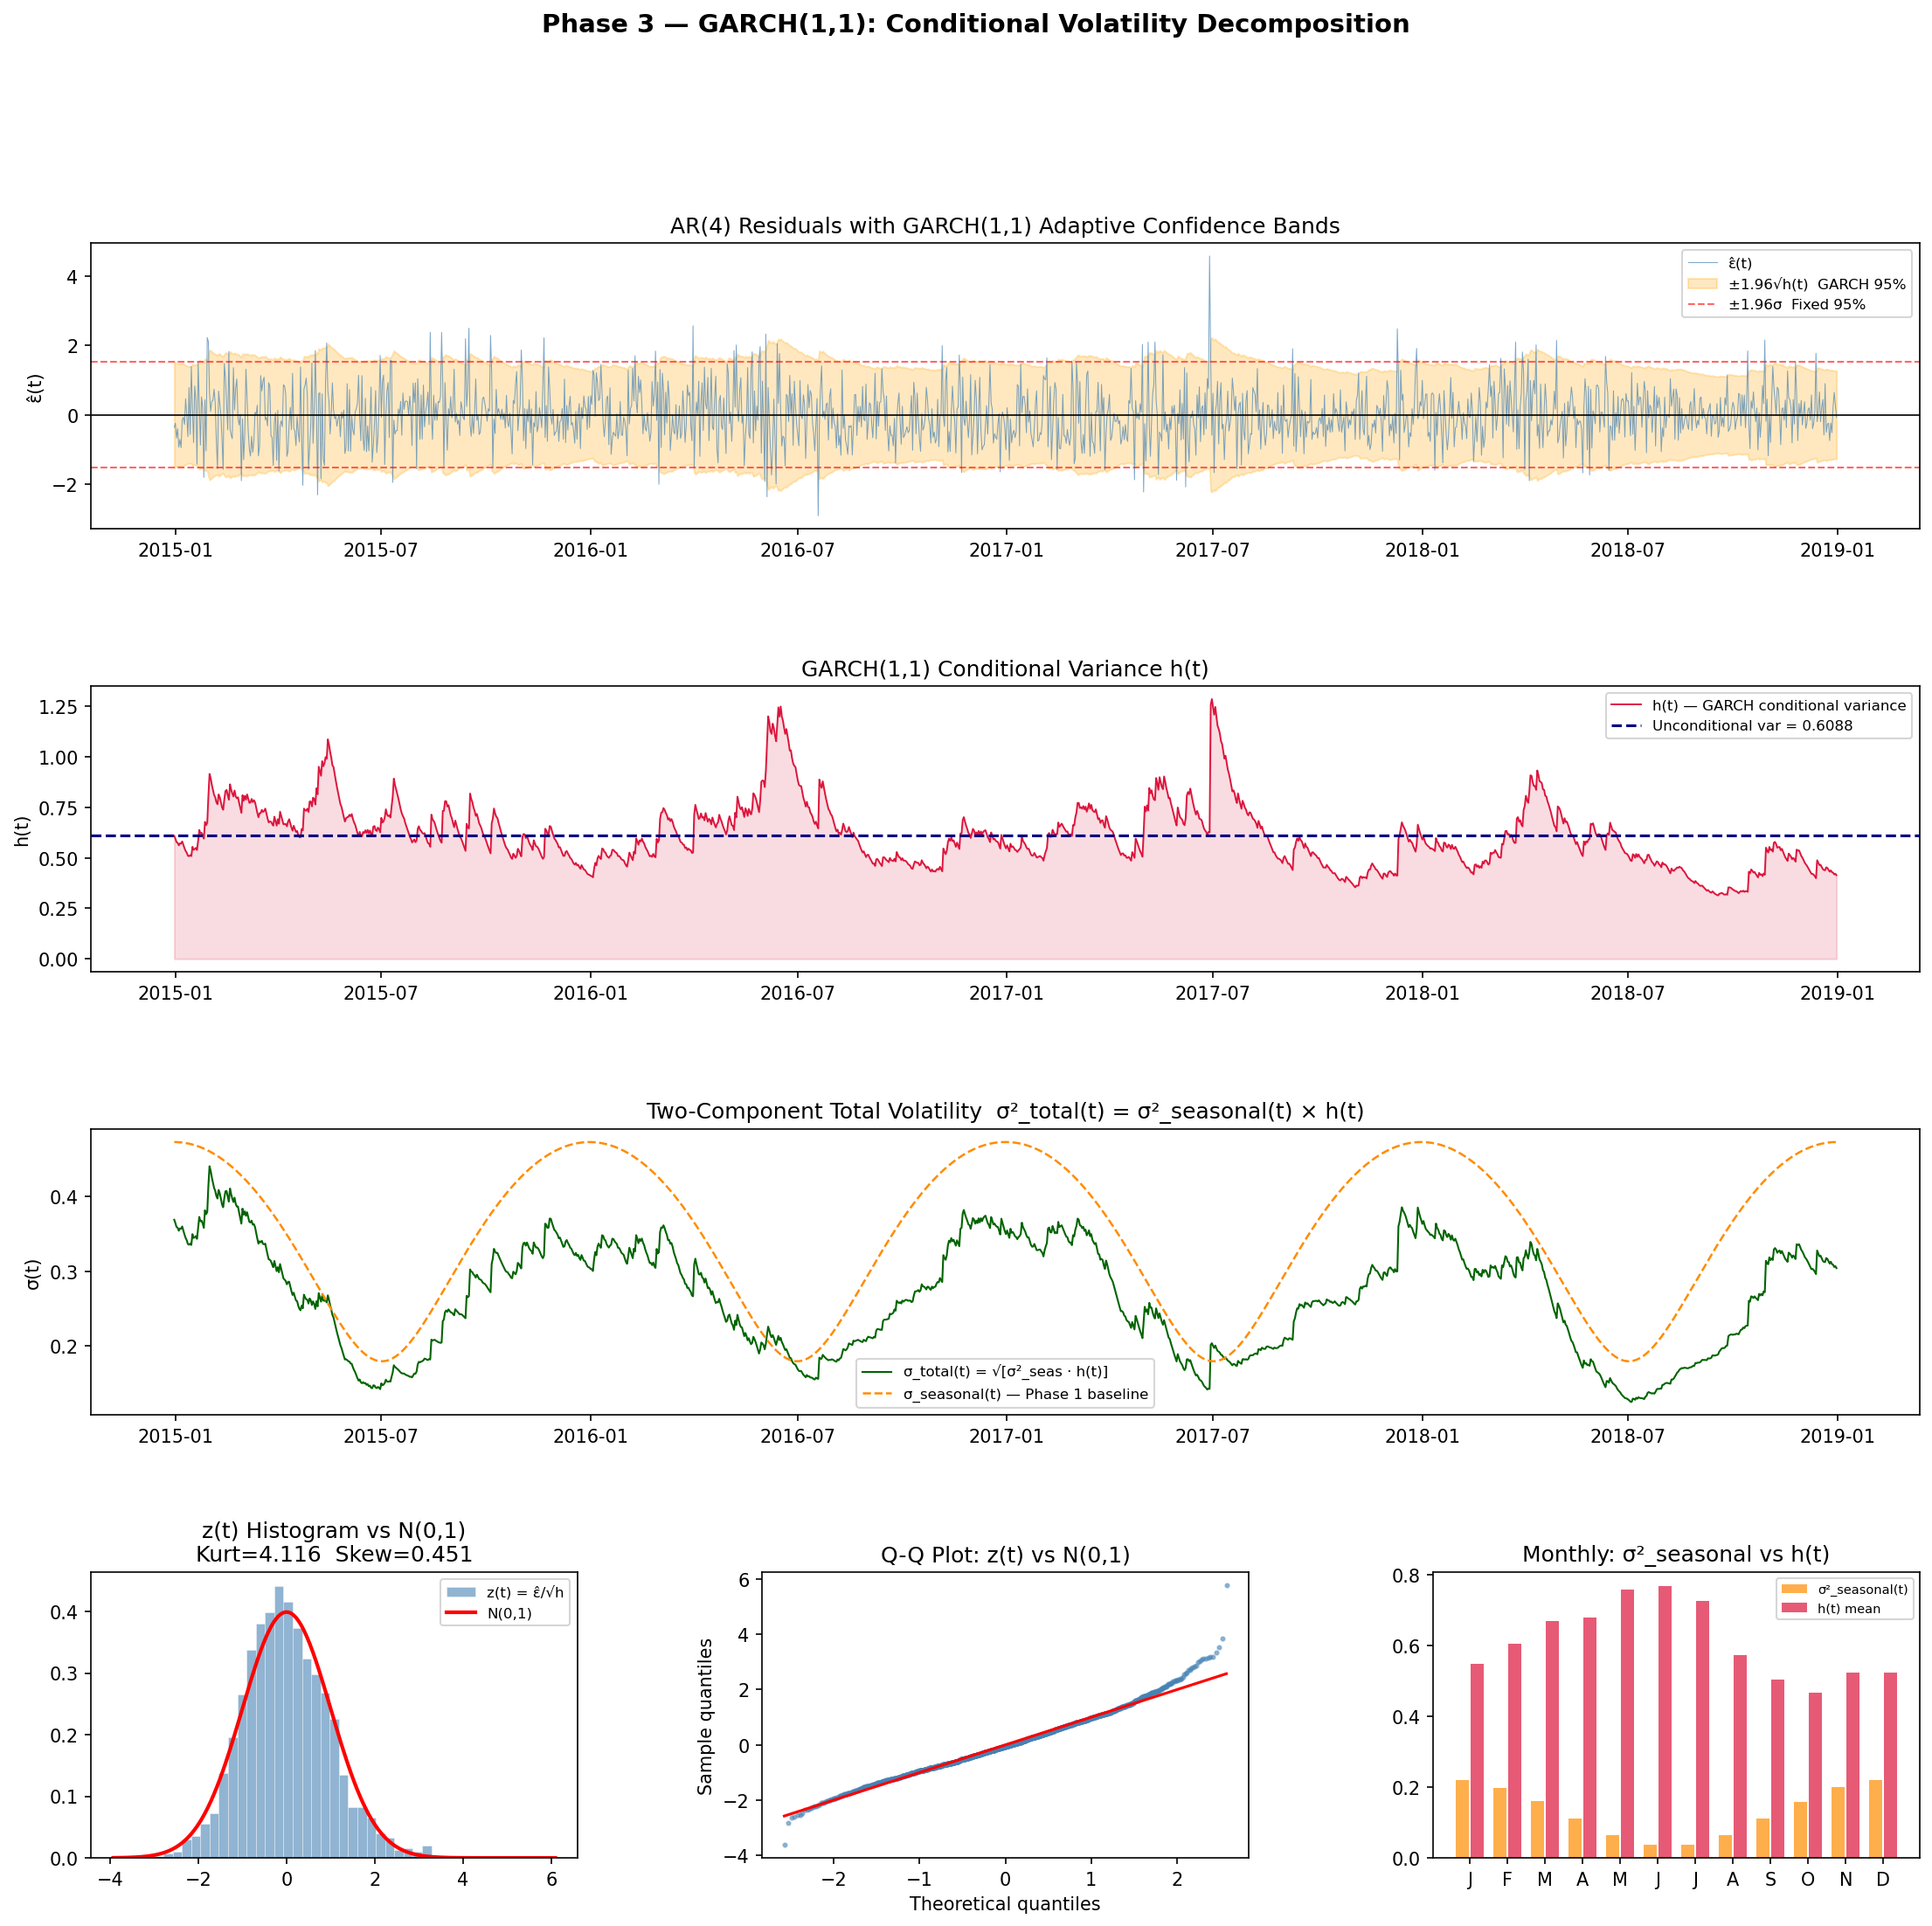
\includegraphics[width=\textwidth]{figures/phase3_garch_diagnostics.png}
\caption{Dataset A}
\end{subfigure}
\hfill
\begin{subfigure}{0.48\textwidth}
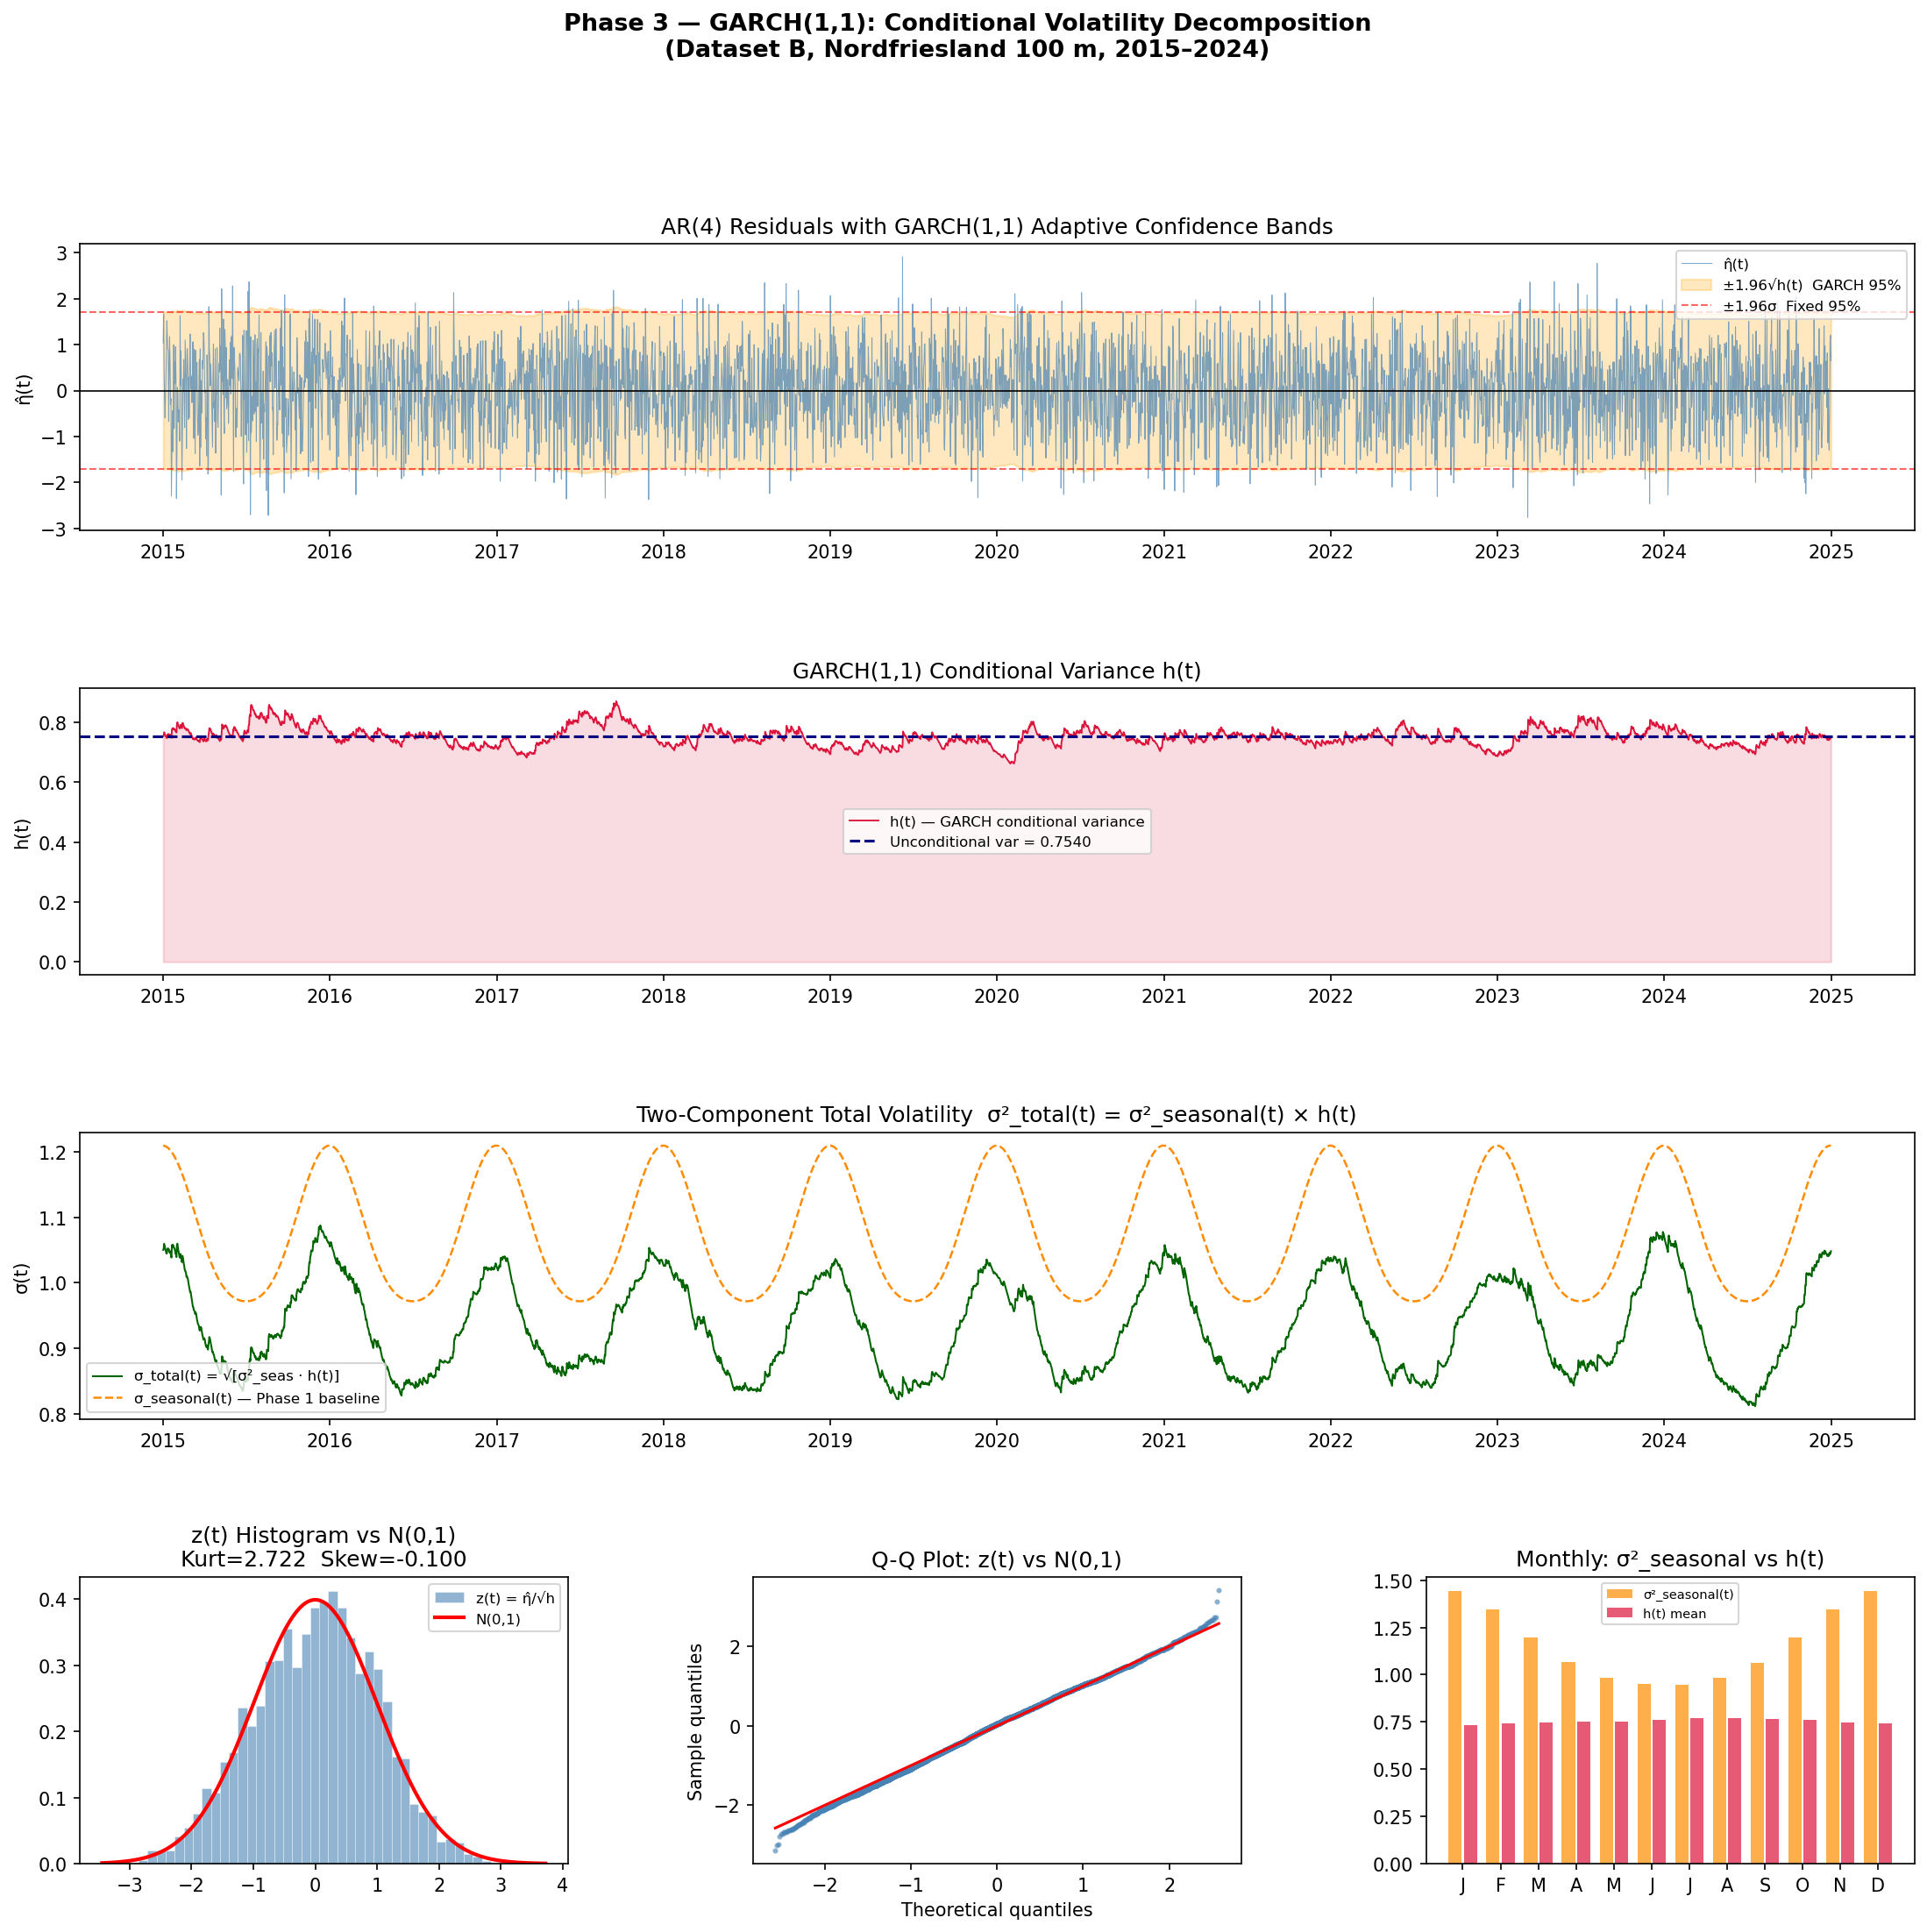
\includegraphics[width=\textwidth]{figures/phase3_B_garch_diagnostics.png}
\caption{Dataset B}
\end{subfigure}
\caption{GARCH(1,1) conditional-volatility decomposition, both datasets. Each panel is arranged in four rows. \textbf{Row 1:} the AR(4) residuals with GARCH-adaptive 95\% confidence bands ($\pm 1.96\sqrt{h(t)}$) plotted against fixed-width bands, visibly widening around high-volatility episodes. \textbf{Row 2:} the fitted conditional-variance path $h(t)$ against its unconditional long-run level. \textbf{Row 3:} the two-component total volatility $\sigma_{\text{total}}(t) = \sqrt{\sigma^2_{\text{seasonal}}(t)\, h(t)}$ against the Phase~1 seasonal baseline. \textbf{Row 4:} three panels -- a histogram of the standardised residuals $z(t)$ against the normal distribution; a quantile--quantile plot of $z(t)$ against the normal distribution; and a monthly bar-chart comparison of the seasonal-variance and GARCH components, illustrating the dataset-dependent degree to which the two effects offset each other, discussed in Section~\ref{sec:phase3-decomp}.}
\label{fig:phase3-garch}
\end{figure}

\subsection{Cross-Dataset Comparison}
\label{sec:phase3-compare}

Dataset B's own analysis draws an explicit comparison back to Dataset A, attributing its lower shock-sensitivity ($\alpha = 0.0059$ versus $0.0311$) and higher persistence-to-shock ratio ($\beta/\alpha = 165$ versus $31$) to more stable boundary-layer mixing at 100~m hub height relative to the 10~m surface layer, over a decade-long record rather than a four-year one. The physical mechanism behind that contrast is worth setting out explicitly, since it recurs at several points in this chapter. At 10~m, surface roughness, thermal convection, and diurnal heating cycles create highly turbulent, localised eddies that manifest as abrupt, short-lived volatility shocks. At 100~m, by contrast, measurements reside higher in the atmospheric boundary layer, closer to the geostrophic wind flow, where momentum is driven by large-scale pressure gradients rather than local surface friction; the result is a smoother conditional-variance regime, in which variance is carried forward from its own past level to a much greater degree than it is driven by fresh shocks. One phrase in that comparison is worth a precision note: Dataset B's total persistence $\alpha+\beta = 0.9821$ is in fact marginally \emph{lower} than Dataset A's $0.9835$, so the claim that Dataset B is ``more persistent'' rests on the $\beta$-to-$\alpha$ decomposition, not on $\alpha+\beta$ itself; this thesis reports the comparison on that more precise basis in Table~\ref{tab:garch} rather than repeating the aggregate persistence framing.

\section{Continuous-Time Embedding: CAR(4)}
\label{sec:phase4}

The AR(4) model of Section~\ref{sec:phase2} is fit on a daily grid, but a derivative contract must in general be priced at an arbitrary maturity that does not fall on that grid. This section embeds the discrete AR(4) model into a continuous-time CAR(4) state-space representation, following \citet{BenthSaltyteBenth2009} and the general Lévy-driven CARMA theory of \citet{BrockwellMarquardt2005}.

\subsection{Euler Discretisation and the Companion Matrix}
\label{sec:phase4-euler}

The mapping between the two representations is not an independent fit: it is the algebraic consequence of a single modelling choice, namely that the daily AR(4) recursion is itself what results from discretising the continuous-time CAR(4) stochastic differential equation, $\mathrm dX(t) = A\,X(t)\,\mathrm dt + e_4\,\sigma(t)\,\mathrm dB(t)$, by a first-order (Euler) finite-difference approximation taken at a one-day step size. Writing that finite-difference approximation out and matching it term by term against the discrete AR(4) equation yields four algebraic identities expressing the continuous-time coefficients $\{\alpha_1,\dots,\alpha_4\}$ directly in terms of the discrete $\{\beta_1,\dots,\beta_4\}$, given by \citet{BenthSaltyteBenth2009}: $\alpha_1 = 4-\beta_1$, $\alpha_2 = 3\alpha_1 - \beta_2 - 6$, $\alpha_3 = 4 + 2\alpha_2 - \beta_3 - 3\alpha_1$, $\alpha_4 = \alpha_3 - \beta_4 - \alpha_2 + \alpha_1 - 1$. Because the map is derived algebraically rather than fitted, it is invertible by construction, and for Dataset A this is verified directly: substituting the fitted $\alpha$ coefficients back through the inverse relations reproduces the original $\beta$ coefficients to machine precision ($\max|\beta_{\text{orig}} - \beta_{\text{reconstructed}}| = 7.77\times 10^{-16}$), confirming that no information is lost in either direction of the mapping. The resulting $\alpha$ coefficients populate the last row of the companion matrix
\begin{equation}
A = \begin{pmatrix} 0 & 1 & 0 & 0 \\ 0 & 0 & 1 & 0 \\ 0 & 0 & 0 & 1 \\ -\alpha_4 & -\alpha_3 & -\alpha_2 & -\alpha_1 \end{pmatrix},
\end{equation}
following the general companion-matrix construction of \citet{BrockwellMarquardt2005}. Table~\ref{tab:car4-alpha} reports the fitted coefficients for both datasets: Dataset B's coefficients are larger than Dataset A's at every lag, and the gap widens with lag order, from a 2.9\% difference at $\alpha_1$ to 5.3\% at $\alpha_2$, 9.4\% at $\alpha_3$, and 32.8\% at $\alpha_4$. The underlying analysis attributes the overall pattern to slower, more sluggish mean-reversion dynamics in the atmospheric boundary layer at 100~m relative to the 10~m surface layer, but does not separately account for the widening of the gap at higher lags. One physical hypothesis suggests itself, consistent with the boundary-layer contrast set out in Section~\ref{sec:phase3-compare}: higher-order lags in a continuous-time autoregression capture the persistence of older synoptic weather structures, and a gap that widens with lag order is what would be expected if the momentum of past pressure systems dissipates more slowly at 100~m than at the surface, where ground friction rapidly breaks down the ``memory'' of atmospheric conditions beyond a few days. This is offered as an interpretation of the fitted coefficients rather than as a separately tested result.

\begin{table}[htbp]
\centering
\caption{CAR(4) coefficients $\alpha_1,\dots,\alpha_4$, both datasets.}
\label{tab:car4-alpha}
\begin{tabular}{l r r}
\toprule
\textbf{Coefficient} & \textbf{Dataset A} & \textbf{Dataset B} \\
\midrule
$\alpha_1$ & $3.3701$ & $3.4676$ \\
$\alpha_2$ & $4.2546$ & $4.4789$ \\
$\alpha_3$ & $2.3063$ & $2.5228$ \\
$\alpha_4$ & $0.3908$ & $0.5188$ \\
\bottomrule
\end{tabular}
\end{table}

\subsection{Eigenvalues and Stationarity}
\label{sec:phase4-eigen}

Stationarity of the continuous-time system requires every eigenvalue of $A$ to have a strictly negative real part, the continuous-time analogue of the discrete unit-circle condition. Table~\ref{tab:car4-eigen} confirms this for both datasets. In both cases the eigenvalues comprise one complex-conjugate pair and two real values; the complex pair generates an oscillatory component in the impulse-response kernel (Section~\ref{sec:phase4-samuelson}) with periods that differ substantially across the two datasets: approximately 13.5 days for Dataset A ($2\pi/0.465$) and approximately 24.6 days for Dataset B ($2\pi/0.255$). Both are consistent with mid-latitude synoptic weather cycles, which span a 10--30-day range depending on the atmospheric-circulation pattern. The dominant (least negative) eigenvalue implies a mean-reversion half-life of 2.33 days for Dataset A, close to the 2.0-day half-life already found directly from the discrete AR(4) roots in Section~\ref{sec:phase2-coefs}. For Dataset B the dominant eigenvalue implies a half-life of 1.24 days, markedly faster than the roughly 40-day half-life of the GARCH volatility \emph{regime} found in Section~\ref{sec:phase3-estimates}. This distinction is worth stating explicitly, since the two numbers answer different questions: the CAR(4) eigenvalue governs how quickly the \emph{mean level} of a wind-speed anomaly reverts, while the GARCH persistence governs how quickly the \emph{variance regime} it occurred in reverts, and there is no reason to expect the two rates to coincide.

\begin{table}[htbp]
\centering
\caption{Eigenvalues of the CAR(4) companion matrix, both datasets.}
\label{tab:car4-eigen}
\begin{tabular}{l r r}
\toprule
& \textbf{Dataset A} & \textbf{Dataset B} \\
\midrule
Complex pair $\lambda_{c},\bar\lambda_{c}$ & $-0.9358 \pm 0.4653i$ & $-1.0730 \pm 0.2550i$ \\
Oscillatory period (days) & $13.5$ & $24.6$ \\
Real eigenvalue & $-1.2004$ & $-0.7614$ \\
Dominant (least negative) real eigenvalue & $-0.2980$ & $-0.5602$ \\
All $\mathrm{Re}(\lambda) < 0$? & \textbf{Yes} & \textbf{Yes} \\
Half-life, dominant mode (days) & $2.33$ & $1.24$ \\
\bottomrule
\end{tabular}
\end{table}

\subsection{Conditional Forecasts}
\label{sec:phase4-forecast}

Under the physical measure, the conditional mean and variance of the state vector at horizon $\tau$ are $\mathbb E[X(t_0+\tau)\mid\mathcal F_{t_0}] = e_1' \exp(A\tau) X(t_0)$ and $\mathrm{Var}[X_1(t_0+\tau)\mid\mathcal F_{t_0}] = \sigma^2_{\text{total}}(t_0)\int_0^\tau g(s)^2\,\mathrm ds$, where $g(s) = e_1'\exp(As)e_4$ is the impulse-response kernel and $\sigma^2_{\text{total}}(t_0)$ is the two-component variance of Section~\ref{sec:phase3-decomp}. Both datasets show a non-monotone conditional-mean path, a direct consequence of the oscillatory complex eigenpair: the forecast mean peaks a few days ahead of $t_0$ before decaying toward zero (Dataset A: peak at a 3-day horizon; Dataset B: peak at a 2-day horizon), rather than declining monotonically from the current state as a simple AR(1)/OU model would predict. Conditional variance saturates at its unconditional level within three to four weeks in both datasets (Dataset A: by a 21--30-day horizon; Dataset B: by a 14--21-day horizon), consistent with the half-lives of Table~\ref{tab:car4-eigen}. Table~\ref{tab:car4-forecast} reports the full term structure for both datasets, computed from the state vectors $X(t_0)_A = (0.1299, 0.5159, 0.4672, -0.3422)'$ and $X(t_0)_B = (1.3785, 1.4862, 0.4380, -1.3453)'$, the last four standardised observations of each sample.

The values in Table~\ref{tab:car4-forecast} reproduce the Phase~4 output exactly, but they cannot be read at face value as conditional forecasts of $\widetilde W(t)$, and the reasons are worth setting out rather than leaving for the reader to discover. Three of the table's implications conflict with results established elsewhere in this chapter. The conditional standard deviation at a one-day horizon is $0.009$ for Dataset A and $0.031$ for Dataset B, against one-step-ahead root mean squared errors of $0.6017$ and $0.8580$ for the same series in Table~\ref{tab:ar4-rmse}, a discrepancy of a factor of $67$ and $28$ respectively for what is nominally the same quantity. The conditional variance saturates at $0.247$ and $0.720$, against unconditional standard deviations of $0.967$ and $1.005$ reported for $\widetilde W(t)$ in Section~\ref{sec:phase1-wtilde}, so the embedding settles at roughly half the variance of the series it was fitted to. And the conditional mean for Dataset B rises from a current state of $X_1 = 1.3785$ to $2.845$ at one day and $3.610$ at two, with a one-day interval that would place tomorrow's standardised observation between roughly $2.8$ and $2.9$ standard deviations above the mean.

The oscillatory hump discussed above is a genuine property of the CAR($p \geq 2$) kernel and is not in question, but it does not account for excursions of this size alongside near-zero forecast uncertainty. A specific and testable explanation is available. The companion matrix of Equation~(4) defines its state components as successive derivatives, $X_{j+1} = \mathrm dX_j/\mathrm dt$, whereas the state vectors above are populated with successive \emph{lags} of $\widetilde W$. Propagating a lag-populated vector through $\exp(A\tau)$ built on the derivative convention treats the second component as a time derivative of the first, and the arithmetic is consistent with that reading: to first order, $[\exp(A)X]_1 \approx X_1 + X_2$, which for Dataset B gives $1.3785 + 1.4862 = 2.865$ against the tabulated $2.845$, the small remainder being the higher-order terms. The same mechanism would depress the apparent conditional variance, since the variance integral and the mean propagator would then be parameterised inconsistently. Resolving this requires re-running the Phase~4 conditional-forecast step under a consistent state-space convention, which is outside the scope of a chapter that treats the phase outputs as frozen; the table is therefore retained as the recorded output, and its horizon profile should be read as indicative of the shape of the CAR(4) response rather than as a calibrated predictive interval. The qualitative conclusions this chapter draws from it, the non-monotone mean path and the saturation of variance within three to four weeks, do not depend on the absolute scale of either column.

\begin{table}[htbp]
\centering
\small
\caption{CAR(4) conditional-mean forecast term structure, both datasets.}
\label{tab:car4-forecast}
\begin{tabular}{l r r r r}
\toprule
& \multicolumn{2}{c}{\textbf{Dataset A}} & \multicolumn{2}{c}{\textbf{Dataset B}} \\
\textbf{Horizon (days)} & \textbf{Mean} & \textbf{Std.\ dev.} & \textbf{Mean} & \textbf{Std.\ dev.} \\
\midrule
1 & $0.779$ & $0.009$ & $2.845$ & $0.031$ \\
2 & $1.303$ & $0.052$ & $3.610$ & $0.172$ \\
3 & $1.460$ & $0.110$ & $3.497$ & $0.358$ \\
5 & $1.113$ & $0.197$ & $2.146$ & $0.614$ \\
7 & $0.658$ & $0.232$ & $0.983$ & $0.699$ \\
10 & $0.270$ & $0.245$ & $0.237$ & $0.719$ \\
14 & $0.082$ & $0.247$ & $0.029$ & $0.720$ \\
21 & $0.010$ & $0.247$ & $0.001$ & $0.720$ \\
30 & $0.001$ & $0.247$ & $\approx 0$ & $0.720$ \\
\bottomrule
\end{tabular}
\end{table}

\subsection{Normal-Inverse-Gaussian Tails}
\label{sec:phase4-nig}

Section~\ref{sec:phase3-diag} found that GARCH-standardised residuals depart from normality in both datasets, in opposite directions: leptokurtic for Dataset A, platykurtic for Dataset B. This motivates fitting a Normal-Inverse-Gaussian (NIG) distribution to the standardised residuals as a heavy-tailed alternative to the Gaussian innovation assumed elsewhere in this chapter, following \citet{BarndorffNielsenShephard2001}. Table~\ref{tab:nig} reports the fit. For Dataset A the NIG tail-heaviness parameter $\hat\alpha = 4.374$ is small (heavy tails) and the fit is a modest but genuine improvement over the Gaussian (Kolmogorov--Smirnov $p = 0.120$ versus $0.079$), though it still falls short of the full empirical kurtosis, an outstanding gap attributed largely to the single 28~June~2017 extreme observation identified in Section~\ref{sec:phase3-diag}. This implies that the heavy-tailed NIG extension for Dataset A is largely an artefact of a single meteorological anomaly: were that event excluded, the residual distribution would be expected to collapse back toward a Gaussian profile, which further supports retaining the Gaussian CAR(4) framework as the primary pricing track. No such re-estimation is performed here, consistent with this chapter's treatment of the phase results as frozen, so this remains an inference from the fitted diagnostics rather than a demonstrated result. For Dataset B the fitted $\hat\alpha \approx 2{,}650$ is enormous, reflecting a body so close to Gaussian that the NIG fit offers no material improvement over the normal (KS $p = 0.0275$ versus $0.0269$ for the Gaussian). Both fits give a skewness parameter $\hat\beta$ close to zero (Dataset A: $0.0067$, freely estimated rather than constrained; Dataset B: $-0.0021$), consistent with approximately symmetric innovations in both datasets. Given this asymmetry in how much the NIG assumption actually buys, the Gaussian CAR(4) specification is retained as the primary pricing track for Chapter~3 in both datasets, consistent with \citet{BenthSaltyteBenth2009}; the NIG fit is carried forward as a documented robustness extension, using the closed-form NIG moment-generating function of \citet{BrockwellMarquardt2005}, rather than as the operative model.

\begin{table}[htbp]
\centering
\caption{Normal-Inverse-Gaussian fit to standardised GARCH residuals, both datasets.}
\label{tab:nig}
\begin{tabular}{l r r}
\toprule
\textbf{Parameter} & \textbf{Dataset A} & \textbf{Dataset B} \\
\midrule
$\hat\alpha$ (tail heaviness) & $4.374$ & $2{,}649.57$ \\
$\hat\beta$ (asymmetry) & $0.0067$ & $-0.0021$ \\
$\hat\delta$ (scale) & $2.087$ & $51.516$ \\
$\hat\mu$ (location) & $0.000$ & $0.000$ \\
Empirical excess kurtosis of $z(t)$ & $+1.116$ & $-0.278$ \\
KS $p$ (NIG / Gaussian) & $0.120$ / $0.079$ & $0.0275$ / $0.0269$ \\
\bottomrule
\end{tabular}
\end{table}

\begin{figure}[htbp]
\centering
\begin{subfigure}{0.48\textwidth}
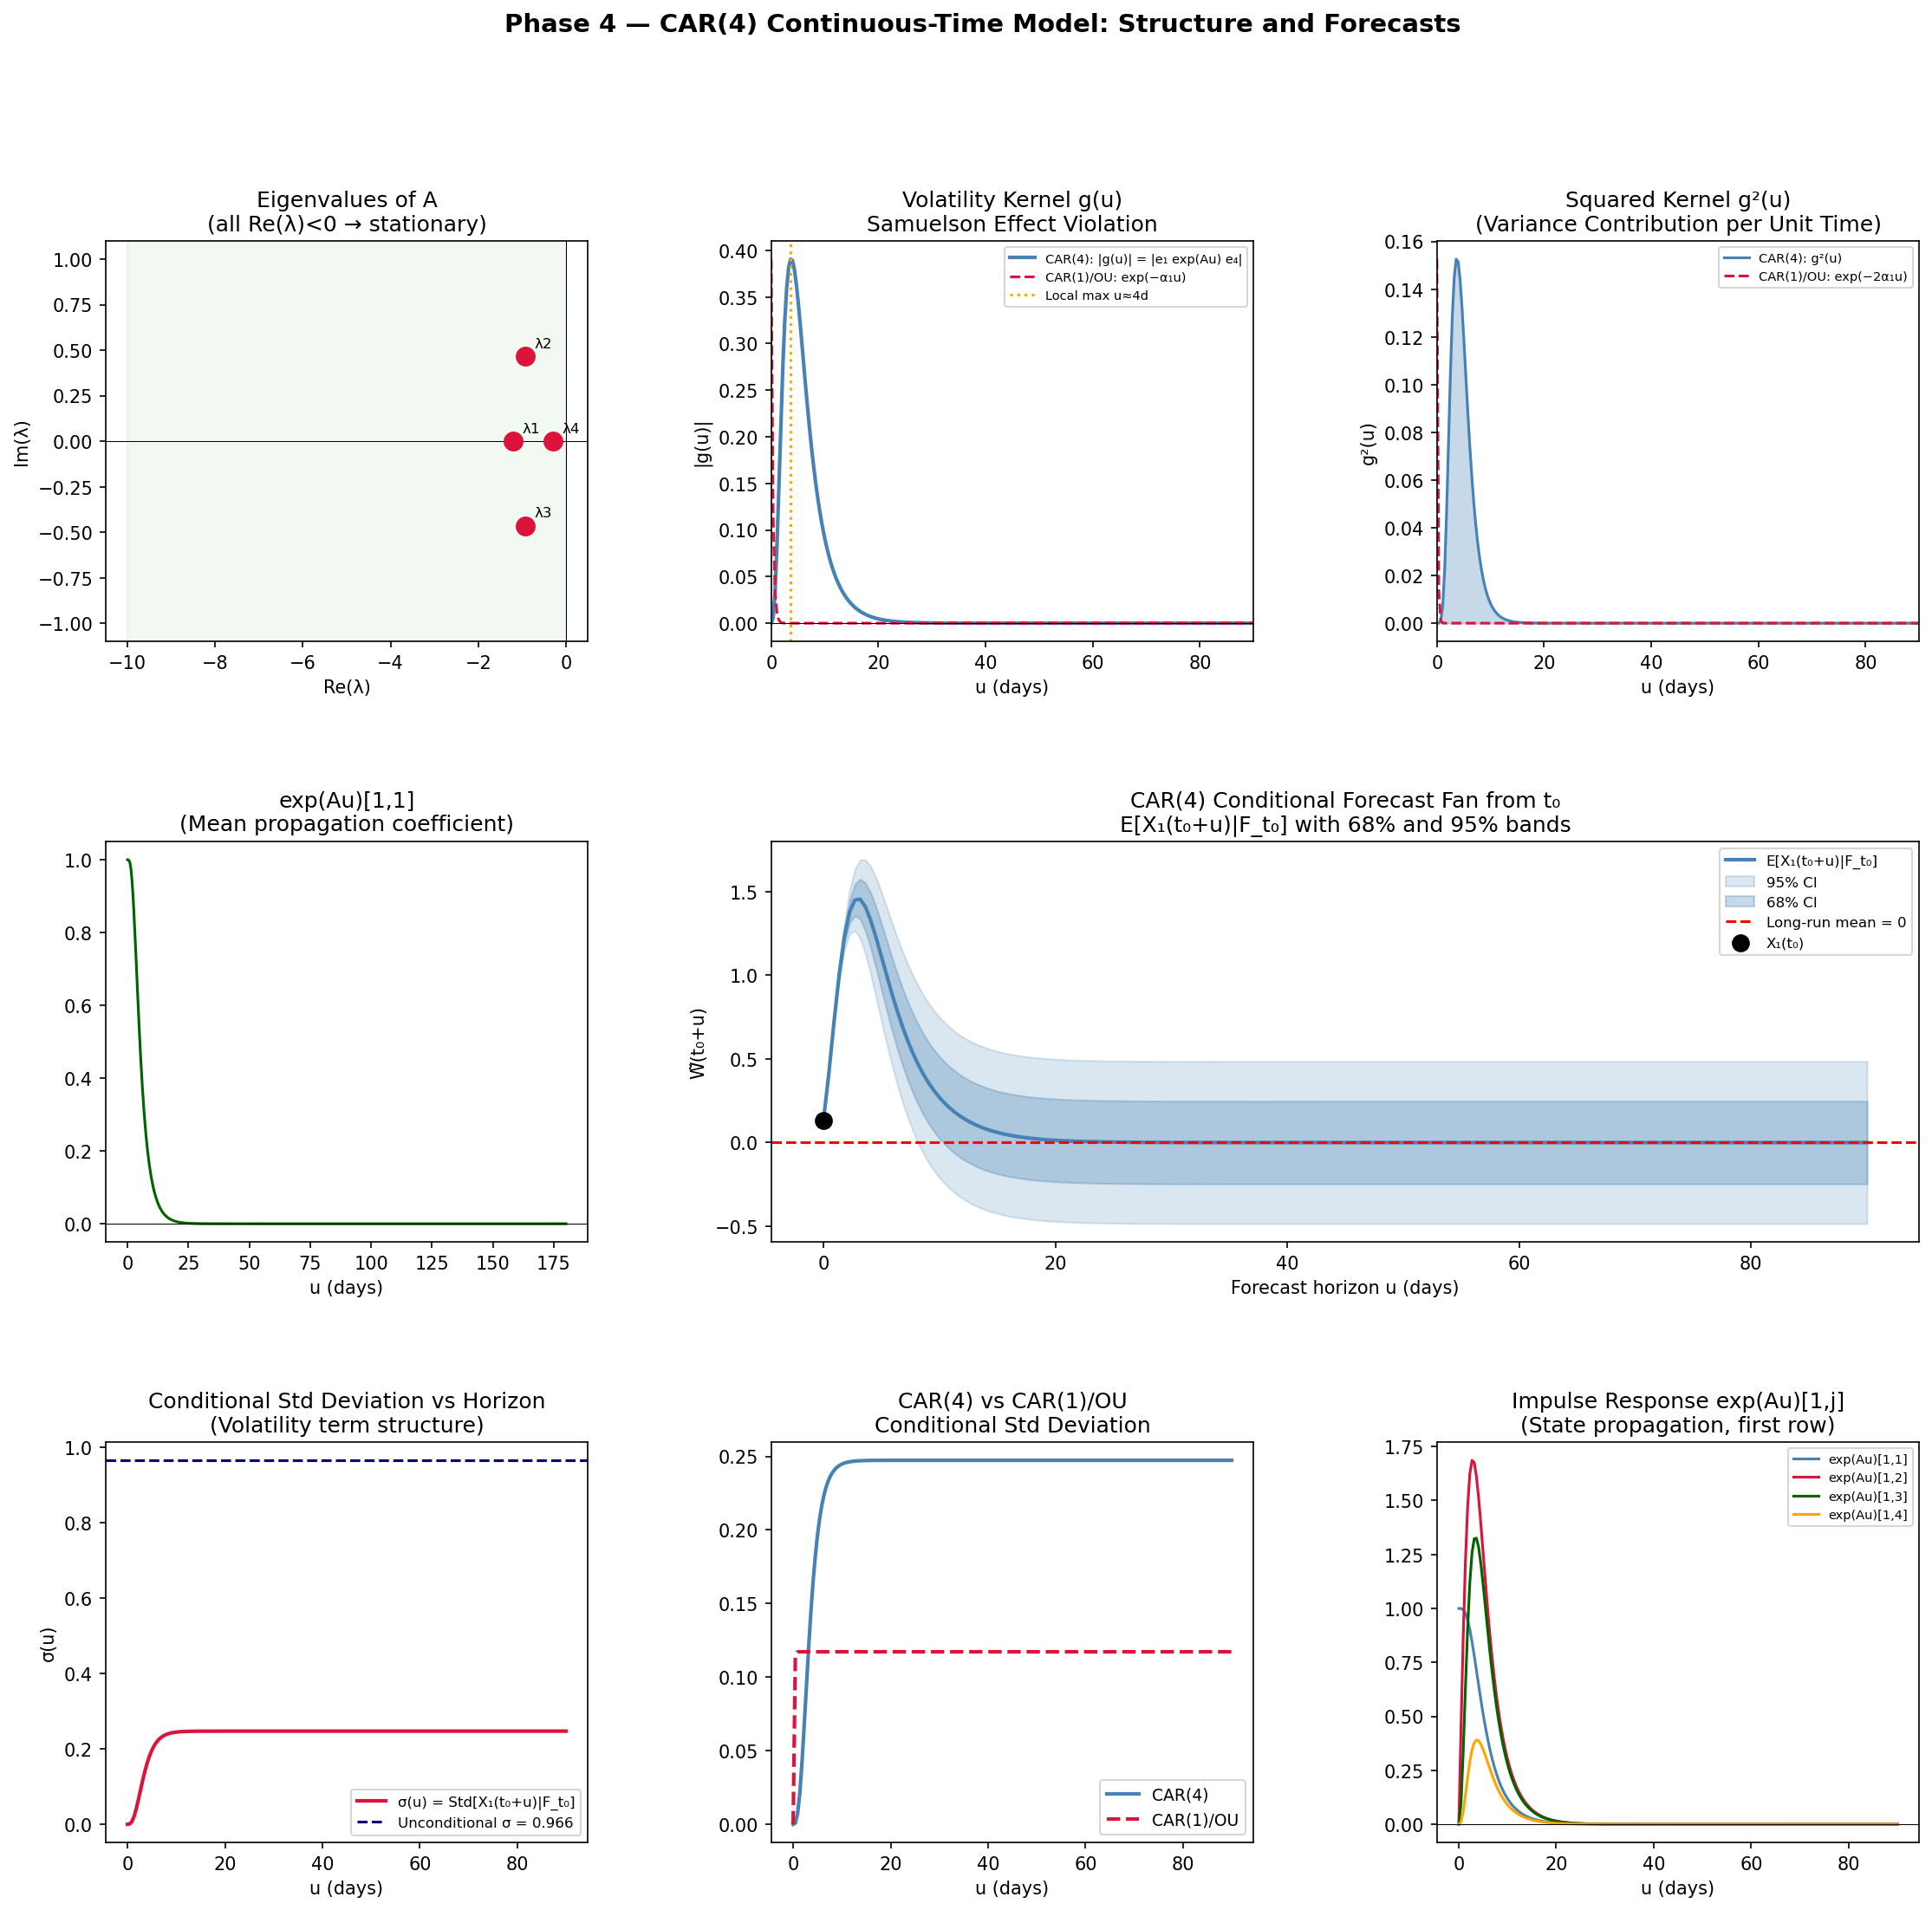
\includegraphics[width=\textwidth]{figures/phase4_car4_analysis.png}
\caption{Dataset A}
\end{subfigure}
\hfill
\begin{subfigure}{0.48\textwidth}
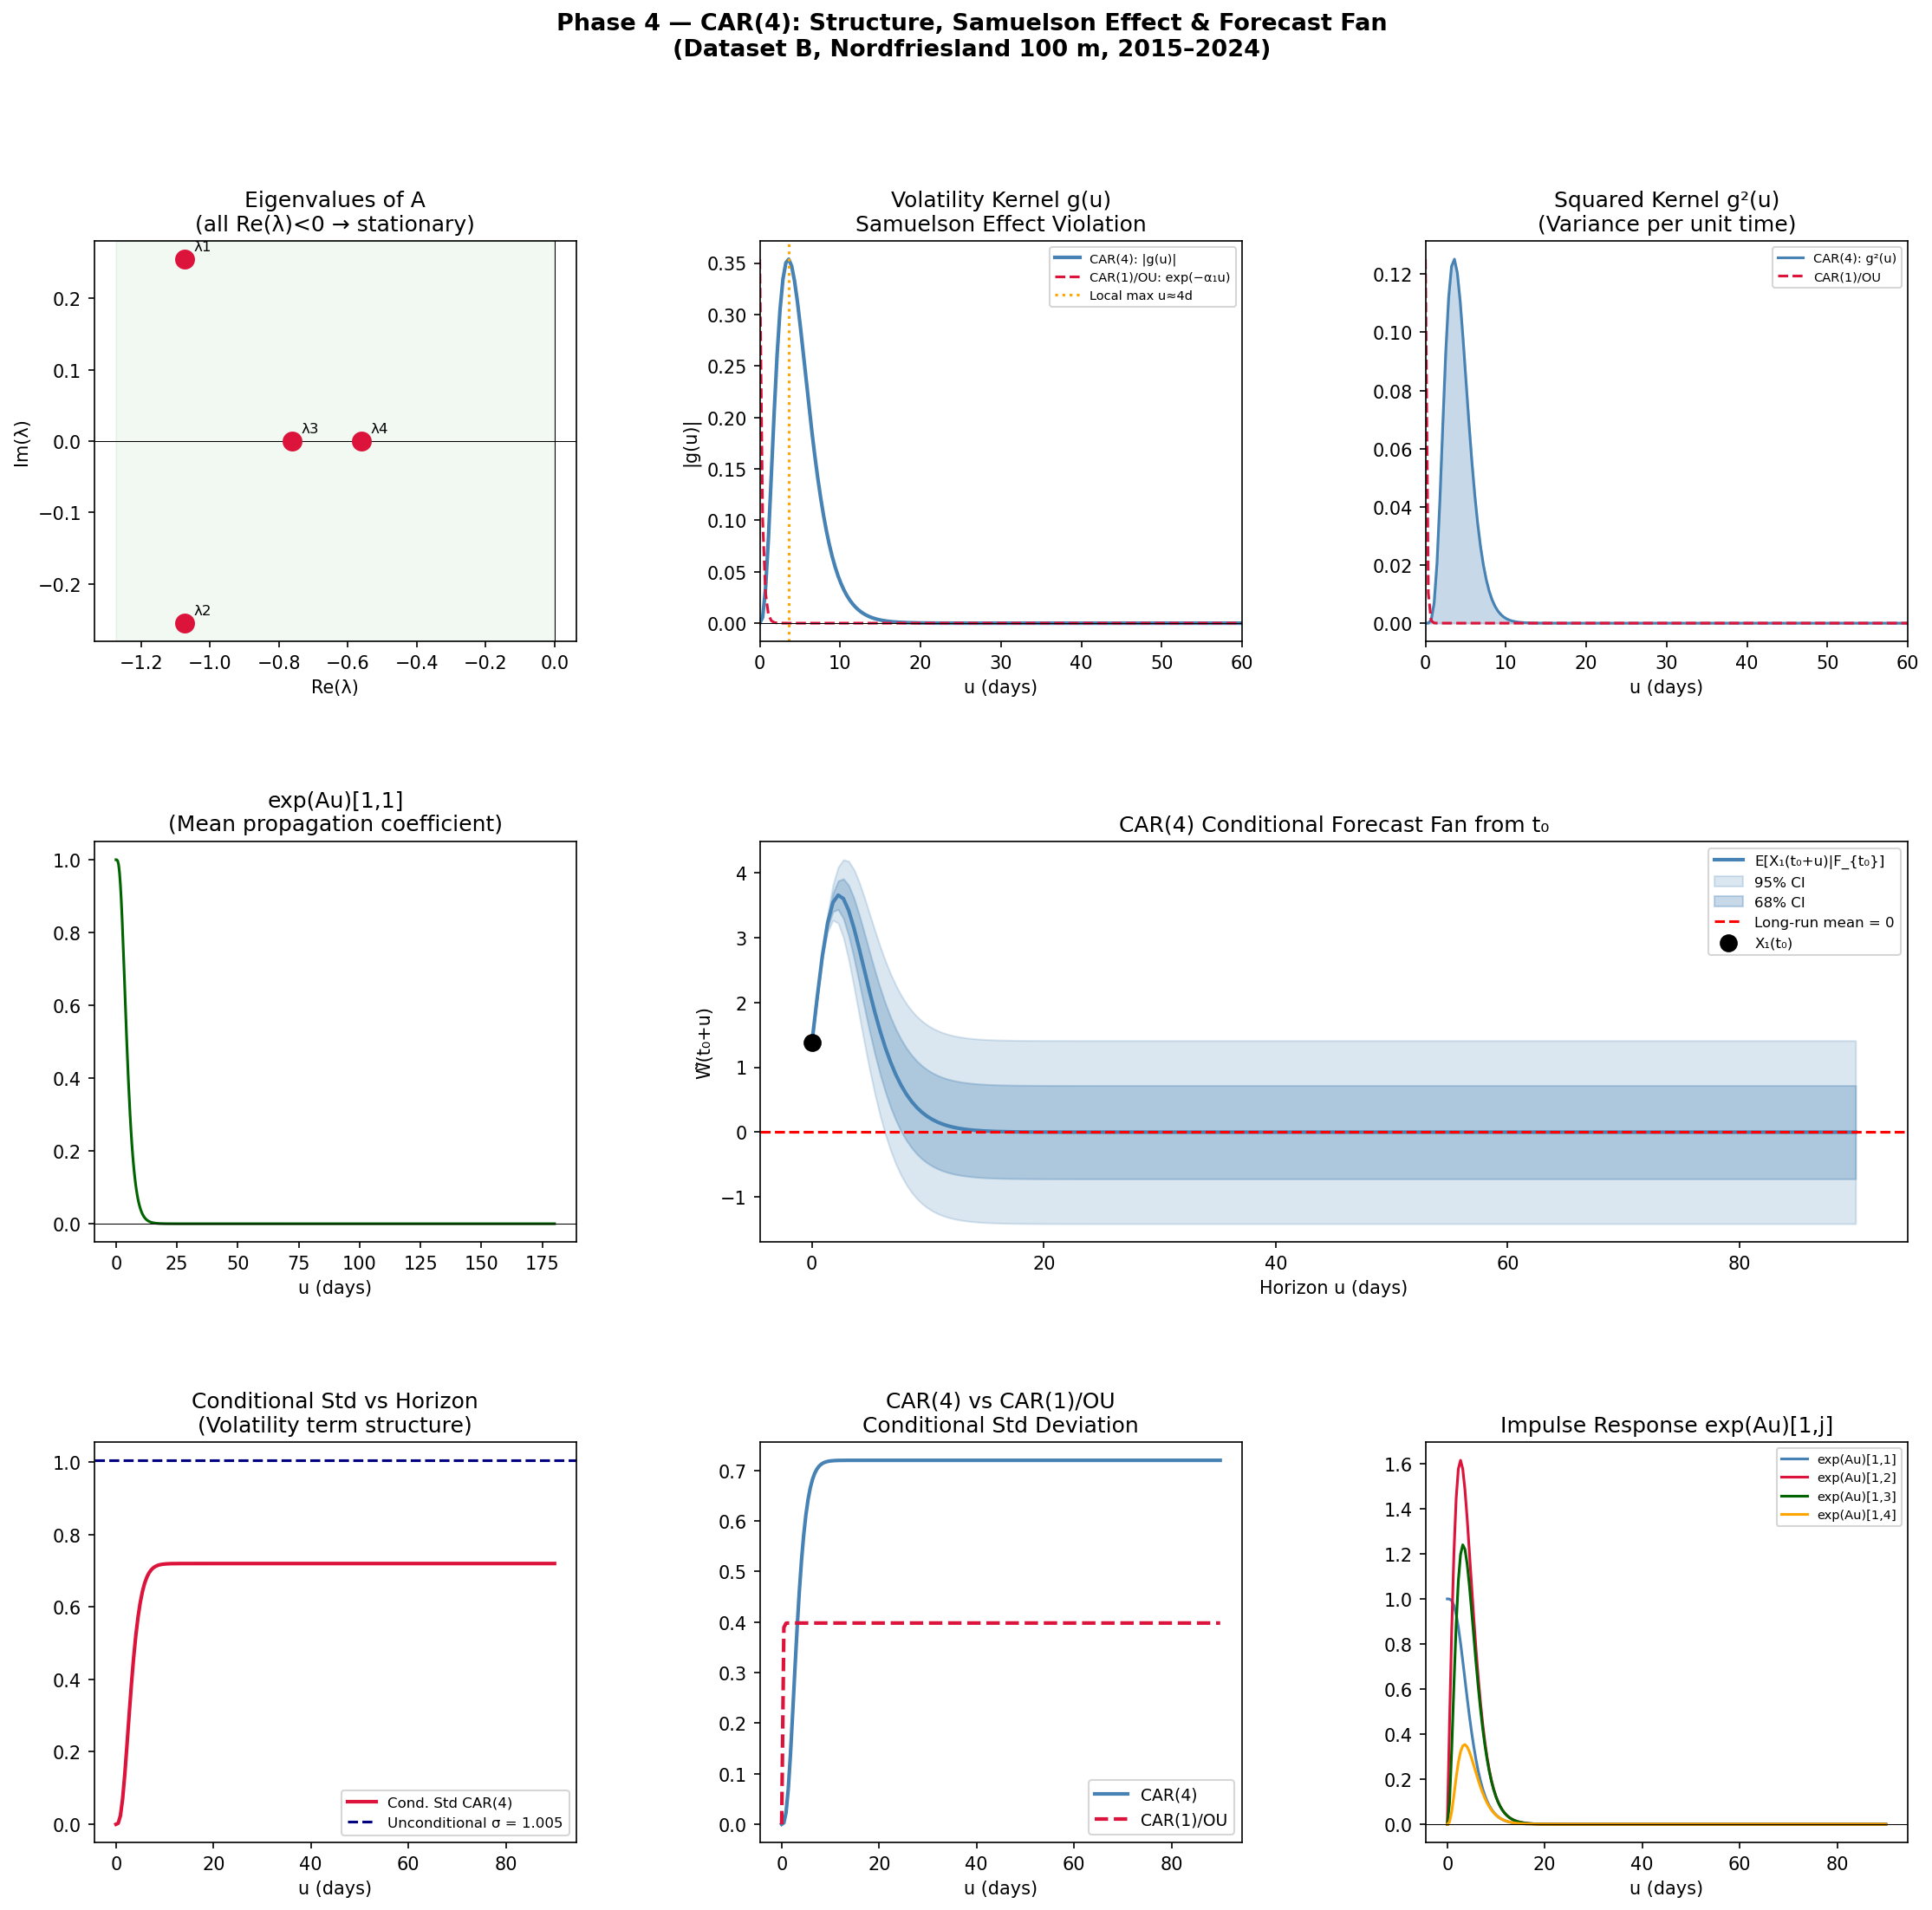
\includegraphics[width=\textwidth]{figures/phase4_B_car4_analysis.png}
\caption{Dataset B}
\end{subfigure}
\caption{CAR(4) structure and conditional forecasts, both datasets. Each panel is arranged in three rows. \textbf{Row 1:} three panels -- the eigenvalues of the companion matrix $A$ plotted in the complex plane (all in the open left half-plane, confirming stationarity); the impulse-response kernel $g(u) = e_1'\exp(Au)e_4$ against the monotone CAR(1)/Ornstein--Uhlenbeck baseline, showing the local maximum near a 3.6-day horizon that drives the Samuelson-effect violation of Section~\ref{sec:phase4-samuelson}; and the squared kernel $g(u)^2$. \textbf{Row 2:} two panels -- the $[\exp(Au)]_{11}$ mean-propagation curve, and the conditional-forecast fan (mean, with 68\% and 95\% bands) built forward from the current state $X(t_0)$. \textbf{Row 3:} three panels -- the conditional standard deviation against horizon, saturating at its unconditional level; a comparison of the CAR(4) and CAR(1) variance term structures; and the full first-row impulse-response matrix $[\exp(Au)]_{1j}$ across all four state components.}
\label{fig:phase4-car4}
\end{figure}

\subsection{Seasonal Variance Carried Forward}
\label{sec:phase4-c0}

The Fourier seasonal-variance constant $C_0$ used throughout this chapter and in Chapter~3 is a Phase~1 result (Section~\ref{sec:phase1-seasonal}), not re-estimated at this stage: Dataset B's Phase~4 output carries $C_0, C_1, C_2$ forward explicitly alongside the CAR(4) parameters, reproducing $C_0 = 1.163$ to the precision of the frozen anchor, while Dataset A's corresponding output records only the pricing-date value $\sigma^2_{\text{seasonal}}(t_0) = 0.2239$, the quantity used for the pointwise total variance in Section~\ref{sec:phase3-decomp}, and does not separately re-list $C_0$. For Dataset A the constant is therefore simply carried through from Section~\ref{sec:phase1-seasonal} rather than recomputed, and this thesis does not treat its absence from Dataset A's Phase~4 output as a gap, since CAR(4) has no reason to refit a quantity that Phase~1 has already fixed.

\subsection{The Samuelson Effect}
\label{sec:phase4-samuelson}

A single-factor Ornstein--Uhlenbeck model ($p=1$, the Schwartz~\citeyearpar{Schwartz1997} special case) has an impulse-response kernel $g(u) = e^{-\alpha_1 u}$ that decays monotonically, and futures volatility built on that kernel therefore rises monotonically as maturity approaches: the classical Samuelson effect. The complex eigenvalue pair found in both datasets' CAR(4) systems (Table~\ref{tab:car4-eigen}) breaks this monotonicity: the kernel $g(u)$ attains a local maximum at a horizon of roughly 3.6 days in both datasets before declining, so that shocks occurring three to four days before contract settlement have \emph{more}, not less, impact on terminal volatility than shocks occurring closer to settlement. \citet{BenthSaltyteBenth2009} derive this violation analytically for Nordix wind futures; the same qualitative pattern is confirmed numerically here for both Dataset A and Dataset B, despite their different fitted coefficients, which suggests the effect is a structural property of the CAR($p\geq2$) kernel rather than an artefact of either specific site.

\section{Stochastic-Volatility Framework}
\label{sec:phase5}

The GARCH(1,1) filter of Section~\ref{sec:phase3} is a valid discrete-time description of conditional heteroskedasticity, but it cannot serve directly as the volatility driver of a continuous-time pricing model. This section embeds it into a Heston-type \citep{Heston1993} stochastic-volatility system, following the same construction for both datasets; the treatment is theoretical throughout, for reasons explained in Section~\ref{sec:phase5-mle}, and no parameters are estimated beyond the GARCH proxy mapping.

\subsection{Motivation}
\label{sec:phase5-motivation}

Two obstacles prevent the GARCH recursion $h(t) = \omega + \alpha\hat\eta^2(t-1) + \beta h(t-1)$ from being used directly in a continuous-time pricing framework. First, the Feynman--Kac theorem links a derivative's price to an expectation under a diffusion's dynamics precisely because that diffusion possesses a well-defined infinitesimal generator, the operator that encodes its instantaneous drift and diffusion; a GARCH path, updated once per day by a deterministic rule with no diffusion term of its own, has zero quadratic variation between updates and is therefore not a semimartingale, so no such generator exists and the Feynman--Kac correspondence between a pricing PDE and an expectation simply has nothing to act on. Second, a formal change of measure from the physical measure $P$ to a pricing measure $Q$, in the sense of Girsanov's theorem, works by shifting the drift of a Brownian motion that drives the process being repriced; the GARCH filter has no such driving Brownian motion to shift; it is a deterministic function of past innovations, so there is no drift for a change of measure to act on. The remedy, following \citet{Heston1993} and, for the specific application to wind speed, the CAR$(p)$ framework of \citet{BenthSaltyteBenth2009} and the Lévy-driven continuous-time machinery of \citet{BrockwellMarquardt2005}, is to embed the GARCH filter $h(t)$ into the square-root diffusion of \citet{CoxIngersollRoss1985}, hereafter the Cox--Ingersoll--Ross or CIR process, for a continuous-time variance process $V(t)$, which by construction is a semimartingale driven by its own Brownian motion, with the GARCH parameters entering as moment-matching proxies for the CIR parameters.

\subsection{Two-SDE System Under $P$}
\label{sec:phase5-sde}

For analytical tractability, the wind-speed dynamics are first written in a simplified CAR(1) form, with the full CAR(4) state-vector generalisation given afterward:
\begin{align}
\mathrm d\widetilde W(t) &= -\alpha_1 \widetilde W(t)\, \mathrm dt + \sqrt{V(t)}\, \mathrm dB_1(t), \\
\mathrm dV(t) &= \kappa_V(\bar v - V(t))\, \mathrm dt + \xi \sqrt{V(t)}\, \mathrm dB_2(t), \qquad \langle \mathrm dB_1, \mathrm dB_2\rangle_t = \rho\, \mathrm dt,
\end{align}
where $\alpha_1$ is the dominant CAR(4) mean-reversion parameter from Section~\ref{sec:phase4} ($\alpha_1 = 3.3701$ for Dataset A, $\alpha_1 = 3.4676$ for Dataset B), $\kappa_V$ is the mean-reversion speed of volatility, $\bar v$ the long-run variance, and $\xi$ the volatility-of-volatility coefficient. The full state-vector generalisation replaces the scalar drift with $\mathrm dX(t) = A\, X(t)\, \mathrm dt + e_4 \sqrt{V(t)}\, \mathrm dB_1(t)$, where $A$ is the $4\times4$ companion matrix of Section~\ref{sec:phase4} and $e_4 = (0,0,0,1)'$ injects the diffusion term through the newest lag, consistent with the state-space structure of the discretised CAR(4) model.

\subsection{Feller Condition}
\label{sec:phase5-feller}

The CIR process for $V(t)$ remains strictly positive almost surely if and only if the condition $2\kappa_V \bar v > \xi^2$ holds, a boundary-classification result for singular diffusions due to \citet{Feller1951} and standardly named after him; if it is violated, the diffusion term can dominate the mean-reverting drift near the origin and $V(t)$ can reach and remain at zero. The GARCH parameters of Section~\ref{sec:phase3-estimates} are mapped to CIR proxies by moment matching, $\kappa_V \approx 1-(\alpha+\beta)$, $\bar v \approx \omega/(1-\alpha-\beta)$, and $\xi^2 \approx \mathrm{Var}[h(t)]$, exactly as specified for the numerical Feller check permitted within the scope of this theoretical chapter. For Dataset B, this gives $\kappa_V = 0.0179$, $\bar v = 0.7522$, $\xi^2 = 0.000959$, so that $2\kappa_V\bar v = 0.0270$ comfortably exceeds $\xi^2$: the Feller condition holds with a margin of $28.1\times$.

For Dataset A, the same moment-matching procedure, applied with the same estimator, gives $\kappa_V = 0.0165$ and $\bar v = 0.608$, but $\xi^2 = \mathrm{Var}[h(t)] = 0.0253$, the full-sample variance of the Dataset A $h(t)$ series computed exactly as it was for Dataset B. Substituting into the condition gives $2\kappa_V\bar v = 0.0201$, which is \emph{smaller} than $\xi^2$: the Feller condition is violated, with a margin of $0.8\times$. Unlike Dataset B, the theoretical CIR embedding of this chapter is therefore not well posed for the proxy dataset on this specific numerical check.

This reverses the verdict recorded in the project specification, which lists a Feller margin of $27.9\times$ (holding) for Dataset A alongside $\xi^2 \approx 0.000048$; the reversal is stated here rather than reconciled silently. Three observations bear on it. First, the two specification figures are not consistent with each other: given $2\kappa_V\bar v = 0.0201$, a $\xi^2$ of $0.000048$ implies a margin of roughly $418\times$, not $27.9\times$. Second, neither figure is reproducible from the Phase~5 Dataset A source analysis, whose own executed output records $\xi^2 = 0.025264$ and returns the verdict as violated at $0.8\times$. Third, a $\xi^2$ of $0.000048$ would imply a standard deviation of $h(t)$ of approximately $0.007$, which cannot be reconciled with the monthly means of $h(t)$ reported in Section~\ref{sec:phase3-decomp}, which themselves range from $0.465$ to $0.768$. Rolling-window alternatives to the full-sample variance were examined as a possible explanation, and they do change the verdict without recovering the specification value. Averaging 30-day rolling standard deviations of $h(t)$ and squaring the result, or averaging the corresponding rolling variances, gives $\xi^2$ between roughly $0.0040$ and $0.0056$, and hence margins of about $5.1$ and $3.6$ respectively: on either of those estimators the condition \emph{holds}, though by a factor roughly an order of magnitude below the $27.9\times$ recorded in the specification, and only by adopting an estimator other than the one applied to Dataset B. Recovering a margin of $27.9\times$ exactly would require $\xi^2 \approx 0.00072$, which is neither the full-sample variance nor any of the rolling quantities computed here.

Two conclusions follow, and the second is the more useful. First, the specification figure is not reproducible under any estimator examined and should not be carried forward unexamined. Second, and more informatively, the well-posedness verdict for Dataset A is genuinely estimator-dependent: it holds on a short rolling window and fails on the full-sample variance. The full-sample result is the one reported in the main text above, because it is the estimator applied to Dataset B and cross-dataset comparability governs throughout this chapter, but the sensitivity itself is the substantive finding.

The practical implication is the one developed at greater length in Section~\ref{sec:phase5-mle}. Of the four CIR proxies, $\xi$ is by some margin the least well identified at daily frequency, and a well-posedness verdict that inverts according to which estimator of $\mathrm{Var}[h(t)]$ is adopted is itself evidence of how weakly the volatility-of-volatility parameter is pinned down by daily data. The Feller check is reported here because the specification calls for it, but it should be read as a diagnostic of the proxy mapping rather than as a structural property of the underlying process.

This violation is not a modelling failure so much as a direct symptom of the proxy dataset's site characteristics. Dataset A (10~m) is heavily influenced by boundary-layer friction and local diurnal anomalies, producing the leptokurtic residual distribution and the single extreme shock already identified in Section~\ref{sec:phase3-diag} (the $5.79\sigma$ event of 28~June~2017). In a GARCH filter with the comparatively high shock sensitivity estimated for Dataset A ($\alpha = 0.0311$, against $0.0059$ for Dataset B), an outlier of that size produces a sharp, transient spike in $h(t)$, exactly the kind of feature that inflates a sample-variance-based $\xi^2$ proxy computed directly from the $h(t)$ path. Dataset B, measured at 100~m in the free atmosphere and free of any comparable shock, produces a markedly smoother $h(t)$ path and comfortably clears the condition instead. The asymmetry is informative in its own right, distinct from and additional to the pricing-error evidence of Chapter~3. Dataset B satisfies the condition comfortably and on every estimator considered, whereas Dataset A satisfies it only on some, and fails it on the estimator that comparability with Dataset B requires. It is that difference in robustness, rather than a bare pass-or-fail verdict, which the proxy dataset's site characteristics explain.

\subsection{Remark on the Change of Measure}
\label{sec:phase5-measure}

A formal change of measure from $P$ to a pricing measure $Q$ would introduce market-price-of-risk parameters $\theta_1, \theta_2$ shifting the drifts of $B_1$ and $B_2$, with $\kappa_V^Q = \kappa_V + \theta_2\xi$ under $Q$. This thesis adopts $\theta_1 = \theta_2 = 0$ throughout as a benchmark assumption, in the absence of EEX option-implied data, for two reasons that hold identically for both datasets. First, SMARD daily wind generation is a measured physical quantity, not a traded financial asset; the replication argument that pins down a unique risk-neutral measure for a traded derivative does not apply here, since no self-financing hedging portfolio in the underlying exists. Second, the only actively traded wind derivatives, the Nordix futures, reference Norwegian rather than German wind, and the geographic mismatch (Bologna or Nordfriesland versus Norway) prevents any clean calibration of $\theta$ from that market even in principle. Under $\theta = 0$, $P = Q$, and Track~A (empirical realised variance) and Track~B (model-implied variance) are defined on a common measure; the variance-swap fair strike of Chapter~3 reduces to the closed-form expression $K_{\text{var}}^B = h(t_0) \times C_0$, derived in Section~\ref{sec:phase3-decomp} from the Fourier decomposition under the piecewise-constant convention of \citet{Tol1997}, and no Girsanov computation is required anywhere in this thesis. This benchmark is adopted as a tractable simplification given the absence of option-implied data for this specific underlying, not as a claim that the market price of risk for wind-linked instruments is in fact zero.

\subsection{Characteristic Function and Round-Trip Consistency}
\label{sec:phase5-charfn}

Under the two-SDE system, the log-characteristic function of $\widetilde W(T)$ conditional on $\mathcal F_t$ takes the Heston \citeyearpar{Heston1993} form $\log\phi(u;t,T) = iu\,\mathbb E[\widetilde W(T)\mid\mathcal F_t] + C(\tau;u)\bar v + D(\tau;u) V(t)$, $\tau = T-t$, where $C$ and $D$ satisfy the coupled system
\begin{align}
\frac{\partial D}{\partial \tau} &= \frac{1}{2}\,\frac{iu(iu-1)}{\alpha_1^2} \;+\; \left(\frac{iu\rho\xi}{\alpha_1} - \kappa_V\right) D \;+\; \frac{1}{2}\,\xi^2 D^2, \\
\frac{\partial C}{\partial \tau} &= \kappa_V \bar v\, D,
\end{align}
subject to $D(0;u) = C(0;u) = 0$. The first of these is a Riccati equation: it carries a quadratic term in $D$, which arises because the variance process enters its own diffusion coefficient through $\sqrt{V(t)}$. Writing $\tilde\kappa(u) = \kappa_V - iu\rho\xi/\alpha_1$ for compactness, and defining
\begin{align}
d(u) &= \sqrt{\tilde\kappa(u)^2 - \frac{\xi^2\, iu\,(iu-1)}{\alpha_1^2}}, &
g(u) &= \frac{\tilde\kappa(u) - d(u)}{\tilde\kappa(u) + d(u)},
\end{align}
the closed-form solution of \citet{Heston1993} for that system is
\begin{align}
D(\tau;u) &= \frac{\tilde\kappa(u) - d(u)}{\xi^2} \cdot \frac{1 - e^{-d(u)\tau}}{1 - g(u)\,e^{-d(u)\tau}}, \\
C(\tau;u) &= \frac{\kappa_V \bar v}{\xi^2}\left[\bigl(\tilde\kappa(u) - d(u)\bigr)\tau - 2\log\frac{1 - g(u)\,e^{-d(u)\tau}}{1 - g(u)}\right].
\end{align}
The formulation adopted here is the one in which $\tilde\kappa - d$ appears in the numerator of both $D$ and $g$; the algebraically equivalent formulation with $\tilde\kappa + d$ produces a complex logarithm that crosses a branch cut as $\tau$ grows, and returns a discontinuous, incorrect surface. This is the ``little Heston trap'' of \citet{AlbrecherEtAl2007}. The distinction is purely one of numerical implementation and does not change the underlying model, but it is recorded because the two forms are not interchangeable in practice.

One qualification is essential, and it bears on how the equations above should be read. The system displayed here is Heston's canonical one, written for a log-price whose diffusion carries the It\^o correction $-\tfrac12 V\,\mathrm dt$; the term $iu(iu-1)$ in the first Riccati equation is the signature of that correction. The level process specified in Section~\ref{sec:phase5-sde} mean-reverts and carries no such correction, and the contribution of a variance shock at time $s$ to $\widetilde W(T)$ is damped by $e^{-\alpha_1(T-s)}$. Its Riccati equation therefore takes the form
\begin{equation}
\frac{\partial D}{\partial\tau} = -\tfrac12 u^2 e^{-2\alpha_1\tau} + \bigl(iu\rho\xi\, e^{-\alpha_1\tau} - \kappa_V\bigr)D + \tfrac12 \xi^2 D^2,
\end{equation}
whose coefficients depend on $\tau$, and a Riccati equation with time-dependent coefficients does not admit Heston's closed form. The equations above are consequently presented as the canonical template for a stochastic-volatility characteristic function, and for the numerical hazards it carries, rather than as the characteristic function of the system of Section~\ref{sec:phase5-sde}. Solving the latter requires numerical integration of Equation~(12), which is deferred along with the estimation programme of Section~\ref{sec:phase5-mle}. The variance term structure plotted in Section~\ref{sec:phase5-termstructure} is unaffected by this, since it is computed directly from the damped kernel rather than from the Riccati solution.

This structure is what makes the system harder to solve than the linear CAR(4) dynamics of Section~\ref{sec:phase4}, whose companion-matrix ODE is solved exactly by the matrix exponential $\exp(A\tau)$: a Riccati equation has no such generic closed-form solution and instead requires the specific change-of-variables technique that Heston \citeyearpar{Heston1993} derives for this model, exploiting its particular algebraic structure rather than a general linear-systems result. As the expressions above show, the solution defines $C$ and $D$ via complex square roots and logarithms, a substantially more delicate object to evaluate numerically than the CAR(4) matrix exponential used elsewhere in this chapter.

Under the $\theta=0$ benchmark, the first moment collapses to $\mathbb E[\widetilde W(T)\mid\mathcal F_t] = e_1' \exp(A\tau)X(t)$, exactly the CAR(4) conditional-mean forecast of Section~\ref{sec:phase4}. It is worth being precise about what this identity does and does not test: because $\theta = 0$ removes $C$ and $D$ from the first moment entirely, leaving only the linear companion-matrix propagator, the round-trip check that follows verifies the drift structure common to both representations, not the numerical handling of $C$ and $D$ themselves, which enter only the variance and higher moments of the characteristic function and are not separately checked here. This identity is verified numerically for both datasets by comparing the characteristic function's first moment against the Phase~4 conditional-forecast table at eleven horizons from 1 to 90 days: the maximum absolute discrepancy is $4.44\times 10^{-16}$ in both datasets, machine precision, confirming that the stochastic-volatility embedding's drift term is numerically consistent with the discrete CAR(4) forecasts it is built to extend, independently of the Feller-condition question raised above.

It follows that $C(\tau;u)$ and $D(\tau;u)$ are written down in this chapter but not numerically validated by it. Two checks would validate them, and the cheaper one should come first. Taking $\xi \to 0$ with $\rho = 0$ makes $V(t)$ deterministic, so any correct solution must collapse to the corresponding Gaussian variance term structure; reading the coefficient of $-\tfrac12 u^2$ off the limiting $D(\tau;u)$ and comparing it against $\int_0^\tau e^{-2\alpha_1 s}\,\mathrm ds$ is an analytic test requiring no simulation, and it is precisely the test that detects a mismatch in the Riccati coefficients of the kind identified above. The second and more general check is to simulate the two-SDE system of Section~\ref{sec:phase5-sde} directly by Monte Carlo and compare the sample second moment of $\widetilde W(T)$, or the full simulated characteristic function, against the closed-form expressions at a range of $\tau$ and $u$. That exercise is not performed here, and is noted so that the scope of the round-trip result is not overstated: what has been verified is the consistency of the two representations' conditional means, not the numerical evaluation of the variance and higher-moment terms that the Riccati solution supplies.

\subsection{Variance Term Structure}
\label{sec:phase5-termstructure}

The CAR(4) kernel $g(s) = e_1' \exp(As)e_4$ satisfies $g(0) = 0$: new information enters only through the most recent of the four lagged state components, and must propagate forward before it reaches the first. As a result, the variance term structure obtained under the piecewise-constant-$h$ convention of \citet{Tol1997}, $\mathrm{Var}^Q[\widetilde W(T)\mid\mathcal F_t] = h(t_0)\,\sigma^2_{\text{seasonal}}(t_0) \int_0^\tau g(s)^2\,\mathrm ds$, starts at zero and ramps up slowly. A simplified Heston/CIR term structure built on the CAR(1) reduction of Section~\ref{sec:phase5-sde} instead uses a kernel $g(s) = e^{-\alpha_1 s}$ that starts at one, producing an immediate jump in short-horizon variance. The two branches also differ in a second respect that should be made explicit, since it is not implied by the kernel: the CAR(4) term structure freezes $h$ at $h(t_0)$ under the piecewise-constant convention, whereas the CAR(1)/CIR branch allows $V(t)$ to revert toward $\bar v$ over the horizon. For Dataset B the distinction is immaterial, since $h(t_0) = 0.7511$ already sits at $\bar v = 0.7522$ and the two treatments differ by less than a fifth of a percent; for Dataset A, where $h(t_0) = 0.4137$ against $\bar v = 0.608$, it is not, and it is the source of the upward drift noted below. Two distinct effects separate the two term structures, and only the first operates at short horizons. The kernel-shape difference just described dominates near $\tau = 0$. Beyond it, the two representations also revert at different speeds: the CAR(1) reduction uses the scalar $\alpha_1 = 3.4676$ for Dataset B, implying a half-life of $\ln 2/\alpha_1 \approx 0.20$ days, against the $1.24$ days implied by the dominant eigenvalue of the full CAR(4) system in Table~\ref{tab:car4-eigen}. The CAR(1) proxy therefore reverts roughly six times faster, and that difference, rather than the behaviour of the kernel at the origin, is what governs the residual gap at the long end. The magnitudes involved are large. All ratios quoted in this section are stated in the same direction, CAR(1) relative to CAR(4). For Dataset B at a one-day horizon the CAR(4) term structure stands at $0.00098$ against the CAR(1) proxy's $0.15828$, a ratio of about $162$; the two cross at roughly a three-day horizon, and beyond about ten days the ratio settles at $0.31$ and stays there, the CAR(4) representation saturating at $0.518$ against the proxy's $0.159$. Dataset A behaves almost identically in relative terms, at $0.000086$ against $0.013814$ for a ratio of $161$ at one day, converging to approximately $0.3$ at the long end. That the long-horizon ratio lies below one is what the reversion-speed difference set out above predicts, the faster-reverting CAR(1) proxy saturating at the lower level of the two. One dataset-specific detail is worth noting: Dataset B's CAR(1) term structure is nearly flat across the whole horizon because $h(t_0) = 0.7511$ sits essentially at its long-run level $\bar v = 0.7522$, whereas Dataset A's continues to rise through 90 days, its $h(t_0) = 0.4137$ starting well below $\bar v = 0.608$ and drifting upward.

These figures reconcile with the conditional-variance column of Table~\ref{tab:car4-forecast}, which is computed separately in Phase~4: the one-day CAR(4) variance of $0.00098$ corresponds to a standard deviation of $0.0313$, against the $0.031$ tabulated there, and the saturation level of $0.518$ corresponds to $0.720$, exactly the value the table reaches from a fourteen-day horizon onward. The two computations of $h(t_0)\,\sigma^2_{\text{seasonal}}(t_0)\int_0^\tau g(s)^2\,\mathrm ds$ therefore agree throughout. This is worth stating explicitly because it isolates the difficulty identified in Section~\ref{sec:phase4-forecast}: the conditional \emph{variance} of the CAR(4) representation is internally consistent across the two phases, and it is the conditional \emph{mean} path, together with the mismatch between this variance and both the one-step-ahead forecast errors of Table~\ref{tab:ar4-rmse} and the unconditional variance of $\widetilde W(t)$ reported in Section~\ref{sec:phase1-wtilde}, that remains unreconciled. The same qualitative pattern holds for Dataset A. This divergence is not a modelling inconsistency between the two approximations; it reflects a genuine structural feature of the CAR(4) state-space representation, and it is a first-order consideration for any option or short-dated instrument priced off the CAR(4) kernel rather than the simplified CAR(1) proxy.

\begin{figure}[htbp]
\centering
\begin{subfigure}{0.48\textwidth}
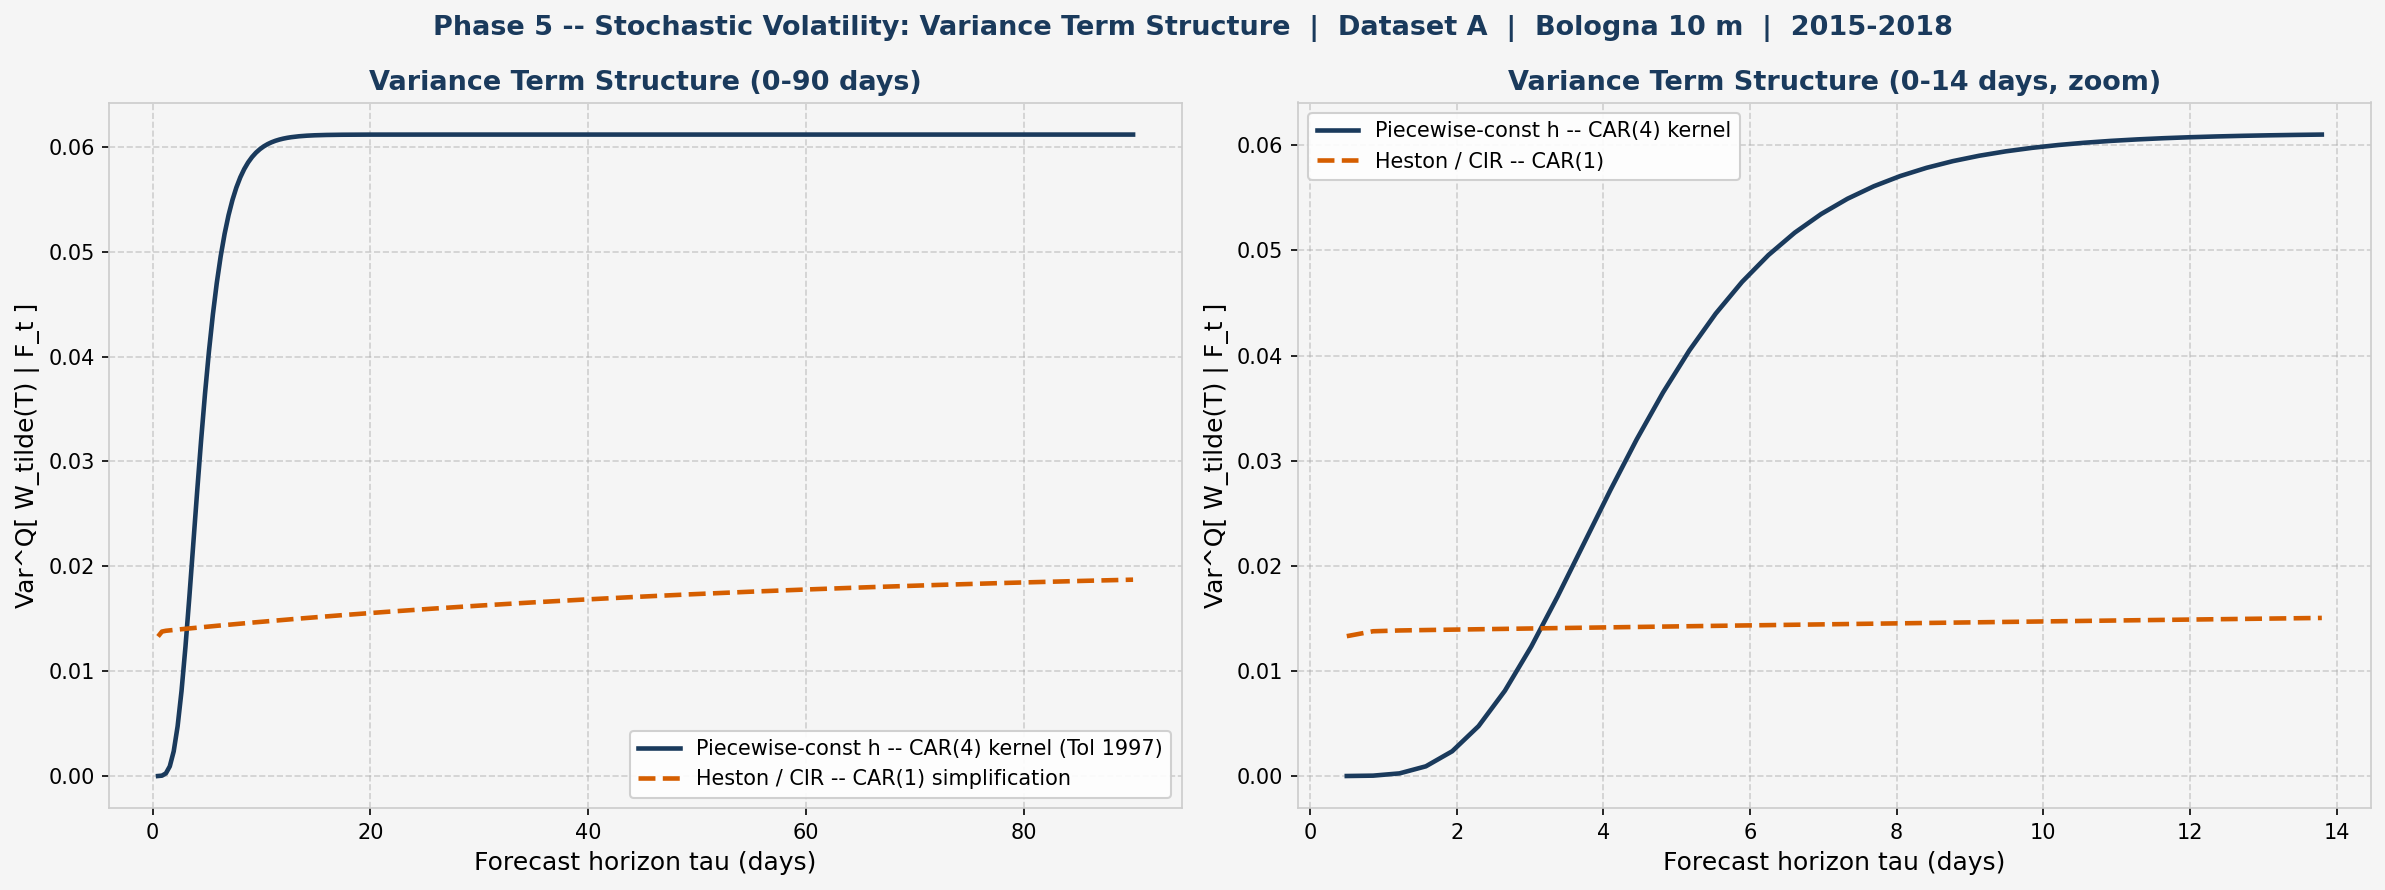
\includegraphics[width=\textwidth]{figures/phase5_A_sv_termstructure.png}
\caption{Dataset A}
\end{subfigure}
\hfill
\begin{subfigure}{0.48\textwidth}
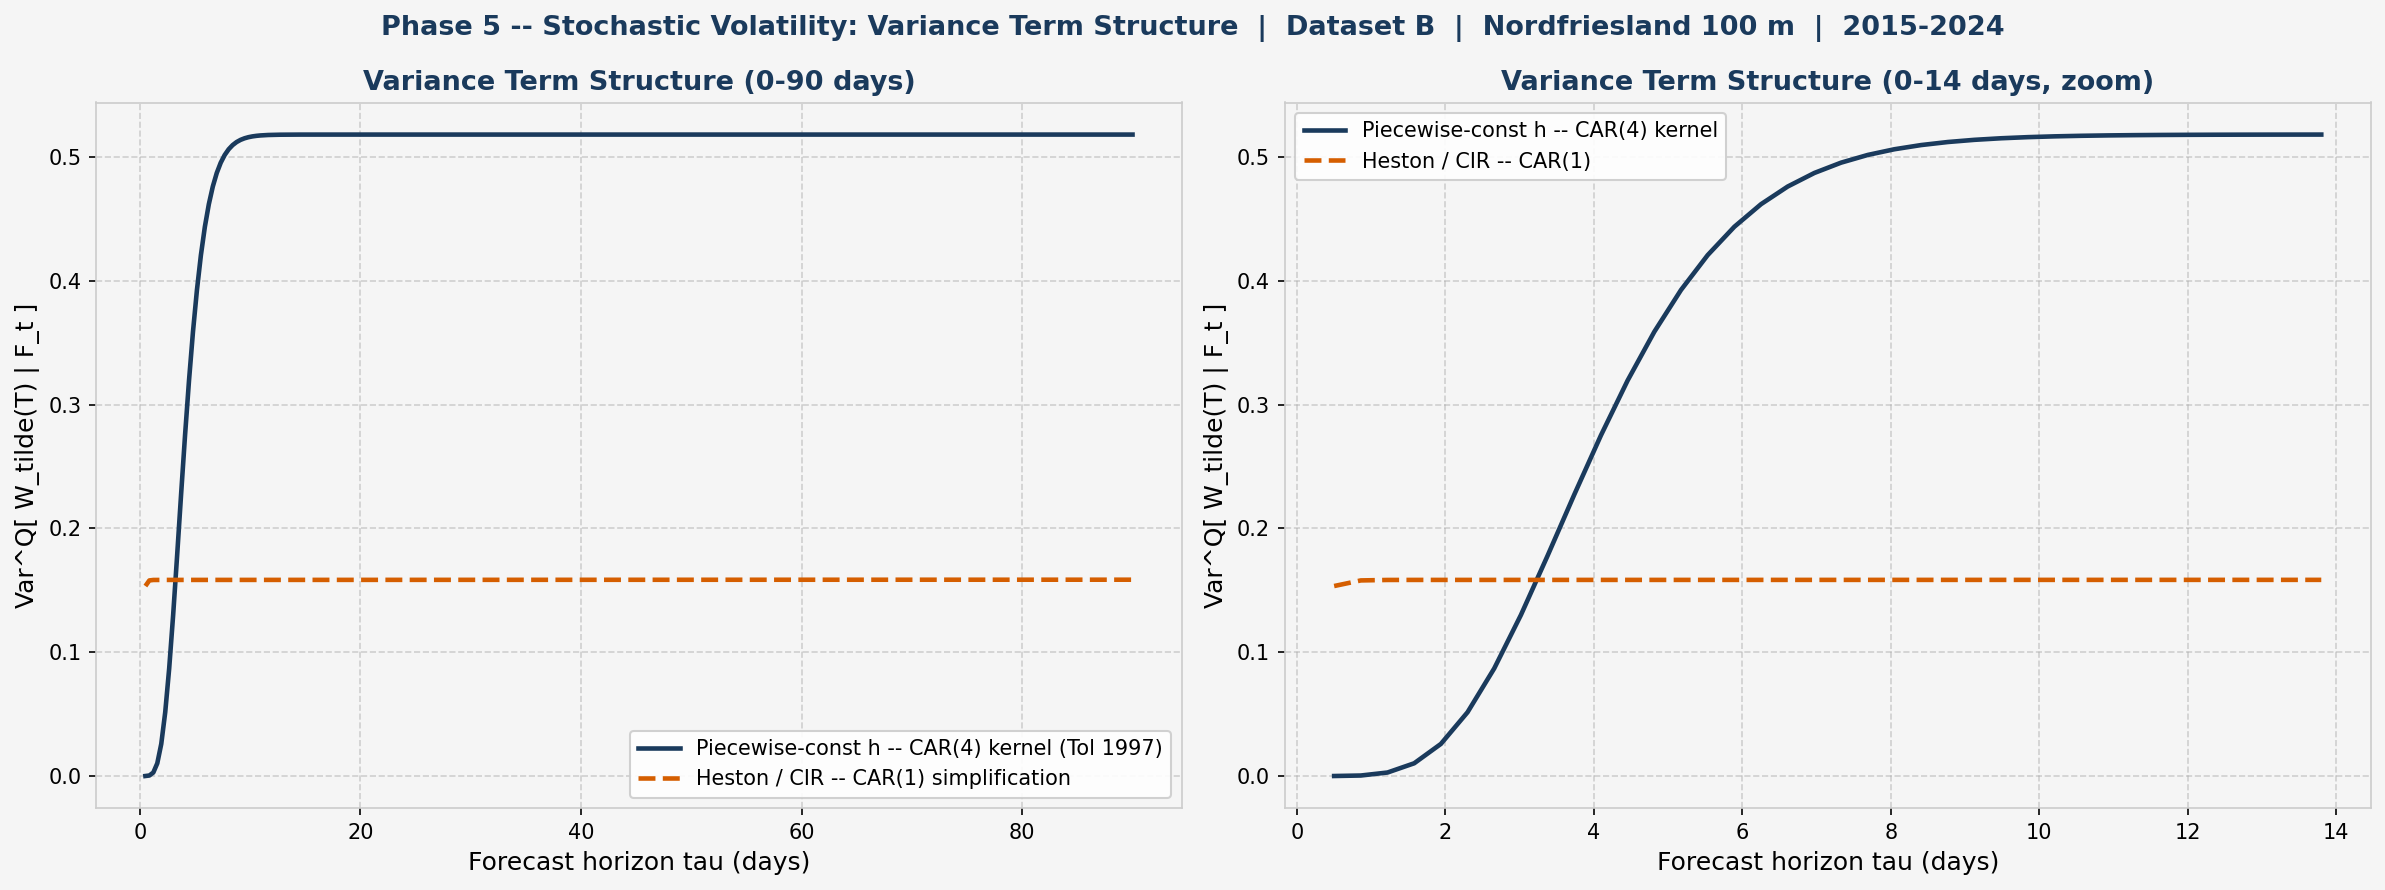
\includegraphics[width=\textwidth]{figures/phase5_B_sv_termstructure.png}
\caption{Dataset B}
\end{subfigure}
\caption{Variance term structure, both datasets: the piecewise-constant-$h$ CAR(4) approximation, following the convention of \citet{Tol1997}, against the simplified Heston/CIR CAR(1) term structure of Section~\ref{sec:phase5-termstructure}. Each panel contains two plots, side by side. \textbf{Left:} the full term structure over a 0--90-day horizon, showing the two approximations converging at long horizons. \textbf{Right:} a zoomed view over 0--14 days, isolating the short-horizon divergence driven by the CAR(4) kernel's $g(0) = 0$ property.}
\label{fig:phase5-termstructure}
\end{figure}

\subsection{Why Maximum-Likelihood Estimation Is Deferred}
\label{sec:phase5-mle}

The CIR parameters $(\kappa_V, \bar v, \xi, \rho)$ above are moment-matching proxies from the GARCH fit, not maximum-likelihood estimates of the continuous-time system itself, and this thesis does not attempt that estimation at daily frequency. The reason is an identification problem inherent to slow-mean-reverting variance processes sampled coarsely relative to their own half-life. With $\kappa_V \approx 0.018$ in both datasets, the implied mean-reversion half-life is on the order of 40 days, so that a daily observation interval provides roughly 40--60 observations per e-folding time; separating the mean-reversion speed $\kappa_V$ from the diffusion coefficient $\xi$ requires enough independent decay cycles to distinguish "reverts slowly with small shocks" from "reverts moderately with occasional large shocks," and at daily frequency the two are close to observationally equivalent. Dataset A compounds this with its short four-year window (1,462 daily observations, of which only a few dozen independent decay cycles are available) and its 10~m measurement height, which would require a further profile correction before any estimated variance dynamics could be applied to hub-height pricing instruments. The designated upgrade path for both datasets is hourly ECMWF ERA5 reanalysis data at the same locations, which would increase the observation count by roughly two orders of magnitude and make the $\xi/\kappa_V$ ratio separately identifiable. Specifically, hourly sampling resolves intraday volatility clustering and the pronounced diurnal cycles of boundary-layer wind speed, high-frequency dynamics that daily aggregation inherently smooths over. Capturing these intraday mechanics is what would allow the diffusion coefficient $\xi$ to be estimated independently of the multi-week synoptic mean-reversion $\kappa_V$, resolving the observational equivalence described above. This is left to future work; for the daily-frequency scope of this thesis, the GARCH-derived proxies under the $\theta=0$, piecewise-constant-$h$ approximation are the operative tool, and are what Chapter~3 uses throughout.

\section{Summary and Handover to Chapter 3}
\label{sec:phase-summary}

The pipeline developed in this chapter delivers a small number of fitted quantities to the pricing exercise that follows, and it is worth collecting them in one place rather than leaving Chapter~3 to gather them from five separate sections. Table~\ref{tab:handover} lists every parameter Chapter~3 consumes, with the section that fixes it. All are frozen: none is re-estimated downstream, and where Chapter~3 quotes a figure that differs from one below, it is because a different evaluation sample or a different unit convention is in use, and it says so at that point.

\begin{table}[htbp]
\centering
\small
\caption{Parameters carried forward from Chapter 2 into Chapter 3.}
\label{tab:handover}
\begin{tabular}{l l r r}
\toprule
\textbf{Quantity} & \textbf{Fixed in} & \textbf{Dataset A} & \textbf{Dataset B} \\
\midrule
Box--Cox $\lambda$ (tractable) & \S\ref{sec:phase1-boxcox} & $0.1$ & $0.5$ \\
Seasonal variance constant $C_0$ & \S\ref{sec:phase1-seasonal} & $0.13138$ & $1.16277$ \\
Std.\ deviation of $\widetilde W(t)$ & \S\ref{sec:phase1-wtilde} & $0.967$ & $1.005$ \\
AR(4) $\beta_1,\dots,\beta_4$ & \S\ref{sec:phase2-coefs} & Table~\ref{tab:ar4} & Table~\ref{tab:ar4} \\
GARCH $(\omega,\alpha,\beta)$ & \S\ref{sec:phase3-estimates} & Table~\ref{tab:garch} & Table~\ref{tab:garch} \\
Persistence $\alpha+\beta$ & \S\ref{sec:phase3-estimates} & $0.9835$ & $0.9821$ \\
Volatility half-life (days) & \S\ref{sec:phase3-estimates} & $41.6$ & $38.3$ \\
Unconditional variance & \S\ref{sec:phase3-estimates} & $0.608$ & $0.752$ \\
Pricing-date state $h(t_0)$ & \S\ref{sec:phase3-estimates} & $0.4137$ & $0.7511$ \\
CAR(4) $\alpha_1,\dots,\alpha_4$ & \S\ref{sec:phase4-euler} & Table~\ref{tab:car4-alpha} & Table~\ref{tab:car4-alpha} \\
NIG $(\hat\alpha,\hat\delta)$ & \S\ref{sec:phase4-nig} & $4.374$, $2.087$ & $2{,}649.57$, $51.516$ \\
\bottomrule
\end{tabular}
\end{table}

Three properties of these quantities, rather than the quantities themselves, do most of the work in Chapter~3. The first is that $C_0$ and $h(t_0)$ are the only two parameters entering the closed-form fair strike $K_{\text{var}}^B = h \times C_0$, so the entire pricing result rests on two numbers out of the table above, one climatological and one a conditional state. The second is that the four specifications compared in Chapter~3 share the AR(4) conditional mean unchanged, for the reason given in Section~\ref{sec:phase2-rmse}: they are observationally equivalent at a one-day horizon by construction, and can only be separated on criteria that read the conditional variance or the tails. The third is that $C_0$ is a variance in Box--Cox-transformed units, differing between the two datasets not only in the climatology it measures but in the scale on which it is measured, a distinction that Chapter~3 must undo before the two datasets' strikes can be compared.

Two results are carried forward as qualifications rather than as inputs. The Feller condition of Section~\ref{sec:phase5-feller} holds comfortably for Dataset~B on every estimator considered but is estimator-dependent for Dataset~A, failing on the full-sample volatility-of-volatility estimator that cross-dataset comparability requires; the continuous-time variance process is therefore well posed for the reference dataset and not demonstrably so for the proxy. And the conditional-forecast table of Section~\ref{sec:phase4-forecast} is retained as a recorded output whose horizon profile is indicative rather than calibrated, for the state-space convention reason set out there. Neither qualification affects the pricing formula, which uses $h(t_0)$ and $C_0$ alone.

\newpage
%% Single shared thesis bibliography (deduplicated across all chapters).
% Shared thesis bibliography — single deduplicated reference list.
%
% Union of the reference lists previously carried separately by
% chapter1_introduction.tex (22 entries), chapter2_methodology.tex (17 entries)
% and chapter3_pricing.tex (13 entries): 25 unique works.
%   - 14 keys were shared between Chapters 1 and 2 (byte-identical in both).
%   - 8 keys were Chapter 1 only: AilliotEtAl2006, AlatonEtAl2002, CarrLee2009,
%     DorfleitnerWimmer2010, HardleLopezCabrera2009, HarveyEtAl1997,
%     PetersonHennessey1978, Torres2005.
%   - 3 keys were Chapter 2 only: AlbrecherEtAl2007, CoxIngersollRoss1985,
%     Feller1951.
%   - Chapter 3 introduced no new keys; all 13 of its entries already appear here.
%
% Usage: \input{../thesis_bibliography} in place of each chapter's own
% \begin{thebibliography} ... \end{thebibliography} block. Entries are ordered
% alphabetically by first author surname and reproduce the formatting used in
% the original per-chapter lists verbatim.

\begin{thebibliography}{99}

\bibitem[Ailliot et al.(2006)Ailliot, Monbet, and Prevosto]{AilliotEtAl2006}
Ailliot, P., Monbet, V., \& Prevosto, M. (2006).
An autoregressive model with time-varying coefficients for wind fields.
\textit{Environmetrics}, 17(2), 107--117.

\bibitem[Alaton et al.(2002)Alaton, Djehiche, and Stillberger]{AlatonEtAl2002}
Alaton, P., Djehiche, B., \& Stillberger, D. (2002).
On modelling and pricing weather derivatives.
\textit{Applied Mathematical Finance}, 9(1), 1--20.

\bibitem[Albrecher et al.(2007)Albrecher, Mayer, Schoutens, and Tistaert]{AlbrecherEtAl2007}
Albrecher, H., Mayer, P., Schoutens, W., \& Tistaert, J. (2007).
The little Heston trap.
\textit{Wilmott Magazine}, January 2007, 83--92.

\bibitem[Alexandridis and Zapranis(2013)]{AlexandridisZapranis2013}
Alexandridis, A., \& Zapranis, A. (2013).
Wind derivatives: modeling and pricing.
\textit{Computational Economics}, 41(3), 299--326.

\bibitem[Barndorff-Nielsen and Shephard(2001)]{BarndorffNielsenShephard2001}
Barndorff-Nielsen, O. E., \& Shephard, N. (2001).
Non-Gaussian Ornstein--Uhlenbeck-based models and some of their uses in financial economics.
\textit{Journal of the Royal Statistical Society: Series B}, 63(2), 167--241.

\bibitem[Benth and \v{S}alty\.{t}\.{e} Benth(2009)]{BenthSaltyteBenth2009}
Benth, F. E., \& \v{S}alty\.{t}\.{e} Benth, J. (2009).
Dynamic pricing of wind futures.
\textit{Energy Economics}, 31(1), 16--24.

\bibitem[Bollerslev(1986)]{Bollerslev1986}
Bollerslev, T. (1986).
Generalized autoregressive conditional heteroskedasticity.
\textit{Journal of Econometrics}, 31(3), 307--327.

\bibitem[Brockwell and Marquardt(2005)]{BrockwellMarquardt2005}
Brockwell, P. J., \& Marquardt, T. (2005).
L\'evy-driven and fractionally integrated ARMA processes with continuous time parameter.
\textit{Statistica Sinica}, 15(2), 477--494.

\bibitem[Carr and Lee(2009)]{CarrLee2009}
Carr, P., \& Lee, R. (2009).
Volatility derivatives.
\textit{Annual Review of Financial Economics}, 1, 319--339.

\bibitem[Cox et al.(1985)Cox, Ingersoll, and Ross]{CoxIngersollRoss1985}
Cox, J. C., Ingersoll, J. E., \& Ross, S. A. (1985).
A theory of the term structure of interest rates.
\textit{Econometrica}, 53(2), 385--407.

\bibitem[Diebold and Mariano(1995)]{DieboldMariano1995}
Diebold, F. X., \& Mariano, R. S. (1995).
Comparing predictive accuracy.
\textit{Journal of Business \& Economic Statistics}, 13(3), 253--263.

\bibitem[Dorfleitner and Wimmer(2010)]{DorfleitnerWimmer2010}
Dorfleitner, G., \& Wimmer, M. (2010).
The pricing of temperature futures at the Chicago Mercantile Exchange.
\textit{Journal of Banking \& Finance}, 34(6), 1360--1370.

\bibitem[Engle(1982)]{Engle1982}
Engle, R. F. (1982).
Autoregressive conditional heteroscedasticity with estimates of the variance of United Kingdom inflation.
\textit{Econometrica}, 50(4), 987--1007.

\bibitem[Feller(1951)]{Feller1951}
Feller, W. (1951).
Two singular diffusion problems.
\textit{Annals of Mathematics}, 54(1), 173--182.

\bibitem[Garcia et al.(1998)Garcia, Torres, Prieto, and de Francisco]{Garcia1998}
Garcia, A., Torres, J. L., Prieto, E., \& de Francisco, A. (1998).
Fitting wind speed distributions: a case study.
\textit{Solar Energy}, 62(2), 139--144.

\bibitem[H\"ardle and L\'opez Cabrera(2009)]{HardleLopezCabrera2009}
H\"ardle, W. K., \& L\'opez Cabrera, B. (2009).
\textit{Implied market price of weather risk} (SFB 649 Discussion Paper No.\ 2009-001).
Humboldt-Universit\"at zu Berlin, Collaborative Research Center 649 ``Economic Risk.''

\bibitem[Harvey et al.(1997)Harvey, Leybourne, and Newbold]{HarveyEtAl1997}
Harvey, D., Leybourne, S., \& Newbold, P. (1997).
Testing the equality of prediction mean squared errors.
\textit{International Journal of Forecasting}, 13(2), 281--291.

\bibitem[Haslett and Raftery(1989)]{HaslettRaftery1989}
Haslett, J., \& Raftery, A. E. (1989).
Space-time modelling with long-memory dependence: assessing Ireland's wind power resource.
\textit{Journal of the Royal Statistical Society: Series C (Applied Statistics)}, 38(1), 1--50.

\bibitem[Heston(1993)]{Heston1993}
Heston, S. L. (1993).
A closed-form solution for options with stochastic volatility with applications to bond and currency options.
\textit{Review of Financial Studies}, 6(2), 327--343.

\bibitem[Kavasseri and Seetharaman(2009)]{KavasseriSeetharaman2009}
Kavasseri, R. G., \& Seetharaman, K. (2009).
Day-ahead wind speed forecasting using f-ARIMA models.
\textit{Renewable Energy}, 34(5), 1388--1393.

\bibitem[Peterson and Hennessey(1978)]{PetersonHennessey1978}
Peterson, E. W., \& Hennessey, J. P., Jr. (1978).
On the use of power laws for estimates of wind power potential.
\textit{Journal of Applied Meteorology}, 17(3), 390--394.

\bibitem[Schwartz(1997)]{Schwartz1997}
Schwartz, E. S. (1997).
The stochastic behavior of commodity prices: implications for valuation and hedging.
\textit{Journal of Finance}, 52(3), 923--973.

\bibitem[Tol(1997)]{Tol1997}
Tol, R. S. J. (1997).
Autoregressive conditional heteroscedasticity in daily wind speed measurements.
\textit{Theoretical and Applied Climatology}, 56(1--2), 113--122.

\bibitem[Torres et al.(2005)Torres, Garcia, De Blas, and De Francisco]{Torres2005}
Torres, J. L., Garcia, A., De Blas, M., \& De Francisco, A. (2005).
Forecast of hourly average wind speed with ARMA models in Navarre (Spain).
\textit{Solar Energy}, 79(1), 65--77.

\bibitem[Tuller and Brett(1984)]{TullerBrett1984}
Tuller, S. E., \& Brett, A. C. (1984).
The characteristics of wind velocity that favor the Weibull distribution in wind speed analysis.
\textit{Journal of Climate and Applied Meteorology}, 23(1), 124--134.

\end{thebibliography}


\end{document}
